\documentclass{thesis}

\title{AppRecommender: um recomendador \\de aplicativos GNU/Linux}
\author{T�ssia Cam�es Ara�jo}
\email{tassia@gmail.com}
\date{\today}
\location{S�o Paulo}
\blurb{
  Instituto de Matem�tica e Estat�stica \\
  Universidade de S�o Paulo \\[1em]
  Disserta��o apresentada ao Programa de P�s-gradua��o \\
  em Ci�ncia da Computa��o para obten��o do \\
  t�tulo de mestre em ci�ncias \\[1em]
  Orientador: Prof. Dr. Arnaldo Mandel
}

\begin{document}
\maketitle
\frontmatter
\begin{abstract}
A crescente oferta de programas de c�digo aberto na rede mundial de
computadores exp�e potenciais usu�rios a in�meras possibilidades de
escolha.\ Em face da pluralidade de interesses destes indiv�duos, mecanismos
eficientes que os aproximem daquilo que buscam trazem benef�cios para eles
pr�prios, assim como para os desenvolvedores dos programas.\ O
\emph{AppRecommender} � um recomendador de aplicativos GNU/Linux que realiza
uma filtragem no conjunto de programas dispon�veis e oferece sugest�es
individualizadas para os usu�rios. Tal feito � alcan�ado por meio da an�lise de
perfis e descoberta de padr�es de comportamento na popula��o estudada, de sorte
que apenas os aplicativos considerados mais suscet�veis a aceita��o sejam
oferecidos aos usu�rios. \keywords{Sistemas de recomenda��o, distribui��es
GNU/Linux}.  \end{abstract}
\selectlanguage{english}
\begin{abstract}
The increasing availability of open source software on the World Wide Web
exposes potential users to a wide range of choices.\ Given the individuals
plurality of interests, mechanisms that get them close to what they are
looking for would benefit themselves and the software developers as well.
\emph{AppRecommender} is a recommender system for GNU/Linux applications
which performs a filtering on the set of available software and individually
offers suggestions to users. This is achieved by analyzing profiles and
discovering patterns of behavior of the studied population, in a way that
only those applications considered most prone to acceptance are presented to
users. \keywords{Recommender systems, GNU/Linux distributions}.
\end{abstract}

\selectlanguage{brazilian}
\cleardoublepage
\pagestyle{ruled}
\tableofcontents
\cleardoublepage
\listoffigures
\cleardoublepage
\listoftables

\mainmatter
\section{Introdu��o} \label{chapter:introducao}

O universo de programas livres e de c�digo aberto oferece aos usu�rios uma
grande amplitude e diversidade de op��es no que diz respeito a aplicativos
para complementar seus sistemas. No entanto, muitas dessas alternativas
permanecem em relativa obscuridade, pois o car�ter majoritariamente n�o
comercial desses sistemas se reflete na aus�ncia de propaganda e outras formas
de divulga��o ostensiva. Desta forma, a descoberta de programas �teis para um
determinado usu�rio por vezes empaca no excesso de informa��es dispon�veis e
organiza��o inadequada. � costume referir-se a esse fen�meno (p. ex.,
\cite{Iyengar:10}) como ``mais � menos'', no sentido de que o aumento da
disponibilidade de escolhas pode confundir o usu�rio e diminuir sua satisfa��o.

Neste contexto de muitas possibilidades onde poucas s�o de fato atrativas, um
sistema capaz de recomendar aplicativos que presumidamente s�o objeto de
interesse de usu�rios exerceria um papel importante. Desenvolvedores se
beneficiariam por meio de um consequente aumento na utiliza��o de seus
programas que, por serem experimentados por mais usu�rios, certamente
receberiam mais relat�rios de erro (\textit{bug reports}), sugest�es e
contribui��es diversas. Para os usu�rios o benef�cio seria alcan�ado de forma
mais direta, dado que poupariam tempo e recursos outrora dedicados a buscas
e filtragens manuais para encontrar os aplicativos mais adequados a seu
ambiente de trabalho.

Tais benef�cios motivaram a concep��o do \textit{AppRecommender}, um
recomendador de aplicativos GNU/Linux desenvolvido no �mbito de um trabalho de
mestrado, cujo objetivo principal � a experimenta��o de diferentes estrat�gias
para recomenda��o no contexto de componentes de software.

O presente trabalho est� organizado da seguinte forma: os cap�tulos
\ref{chapter:distribuicoes} e \ref{chapter:recomendacao} trazem uma breve
introdu��o sobre distribui��es GNU/Linux e sistemas de recomenda��o. O cap�tulo
\ref{chapter:app_recommender} apresenta o AppRecommender como solu��o em
desenvolvimento para o problema exposto. Em seguida, no cap�tulo
\ref{chapter:trabalhos_correlatos} trabalhos correlatos s�o apresentados e, por
fim, o cap�tulo \ref{chapter:conclusao} traz considera��es finais sobre o
trabalho at� a atual etapa de execu��o.

\chapter{Distribui��es GNU/Linux} \label{chapter:distribuicoes}

O contexto hist�rico no qual emergiu o que se conhece hoje por distribui��es
GNU/Linux � abordado a seguir. Especial aten��o � dedicada aos princ�pios de
``empacotamento'' de \textit{softwares} e seus sistemas de gerenciamento,
conceitos que ganharam destaque no processo de consolida��o das principais
distribui��es --- e que guardam estreita rela��o com o presente trabalho.

\section{Surgimento}

Distribui��es GNU/Linux,\index{distribui��es GNU/Linux!conceito} popularmente
conhecidas como \emph{distros}, s�o varia��es do sistema operacional composto
pelo n�cleo Linux (\textit{kernel}) e milhares de aplicativos, cuja base foi
desenvolvida pelo projeto GNU. As primeiras iniciativas neste dom�nio surgiram
em circunst�ncias que favoreciam o desenvolvimento colaborativo, abertura de
c�digo e comunica��o predominantemente por meio da Internet.

O projeto GNU\index{GNU!hist�rico do projeto}\footnote{\url{hhtp://www.gnu.org}} foi criado em 1983 por Richard
Stallman com o objetivo principal de desenvolver um sistema operacional livre em
alternativa ao UNIX\footnote{\url{http://www.unix.org/}} -- solu��o comercial
amplamente difundida na ind�stria -- e que fosse compat�vel com os padr�es
POSIX\footnote{Acr�nimo para \textit{Portable Operating System Interface}.
Fam�lia de normas definidas pelo IEEE com foco na portabilidade entre sistemas
operacionais. \url{http://standards.ieee.org/develop/wg/POSIX.html}}. Nos anos
90 o projeto GNU j� havia atra�do muitos colaboradores, que num curto espa�o de
tempo desenvolveram in�meros aplicativos para compor o sistema operacional. No
entanto, o desenvolvimento do n�cleo do sistema (\textit{GNU Hurd}) n�o
acompanhou o ritmo dos demais aplicativos.

\index{Linux!surgimento}
Em outubro de 1991 o estudante finland�s Linus Torvalds, na tentativa de
atrair colaboradores, publicou c�digo do Freax, o n�cleo de um sistema
operacional desenvolvido por ele na universidade. Anos mais tarde Torvalds declara
que n�o imaginava que aquele projeto desenvolvido sem grandes pretens�es teria
a dimens�o do que hoje se conhece como Linux \cite{Linus:01}.

Com o an�ncio de Torvalds, Stallman vislumbrou a possibilidade de acelerar o
lan�amento do sistema operacional livre se os aplicativos GNU que j� estavam
prontos fossem combinados com o n�cleo rec�m-lan�ado -- de fato, a primeira
vers�o est�vel do GNU Hurd foi lan�ada apenas em 2001. Em 1992 o Linux foi
licenciado sob a GNU GPL\footnote{Acr�nimo para \textit{General Public
License}, � um suporte legal para a distribui��o livre de softwares.} e as
equipes dos dois projetos come�aram a trabalhar na adapta��o do \textit{kernel}
Linux para o ambiente GNU. Este esfor�o conjunto desencadeou o surgimento das
primeiras distribui��es GNU/Linux.

\index{distribui��es GNU/Linux!exemplos}
As distros oferecem diferentes ``sabores'' do sistema operacional, a exemplo do
Debian, Fedora, Mandriva e Ubuntu, que s�o constitu�dos por aplicativos
criteriosamente selecionados por seus desenvolvedores. Tais iniciativas tendem
a reduzir a complexidade de instala��o e atualiza��o do sistema para usu�rios
finais \cite{Cosmo:08}. Os desenvolvedores das distribui��es atuam como
intermedi�rios entre os usu�rios e os autores dos aplicativos, por meio do
encapsulamento de componentes de software em abstra��es denominadas
\textit{pacotes}.

\section{Empacotamento de programas}

\index{empacotamento!conceito}
O termo empacotamento refere-se ao ato de reunir num �nico arquivo (o pacote),
um conjunto de programas execut�veis, bibliotecas, arquivos de configura��o,
documenta��o, e qualquer outro dado necess�rio para a utiliza��o de um programa
no sistema operacional.

As distribui��es que optam por disponibilizar pacotes mant�m uma infraestrutura
de servidores como fonte de distribui��o de programas. Tais servidores,
denominados ``reposit�rios'', podem ser mantidos oficialmente pela distribui��o
ou oferecidos por terceiros, considerados portanto ``n�o oficiais''. Os sistemas
gerenciadores de pacotes, respons�veis por manter uma base consistente de
programas no sistema, s�o configurados para buscar os pacotes a serem
instalados em um determinado conjunto de reposit�rios.

\subsection{Pacotes Debian}

\index{Debian!sistema de empacotamento}
Debian GNU/Linux e distribui��es derivadas, entre elas a
\textit{Ubuntu}\footnote{\url{http://www.ubuntu.com}}, utilizam o
formato de pacote bin�rio \textit{deb}, composto por arquivos execut�veis,
bibliotecas e documenta��o associados a um programa ou conjunto de programas
relacionados. Idealmente, todos os dados e procedimentos necess�rios para
instalar, configurar e remover os aplicativos de um sistema est�o contidos em
seu pacote.

A estrutura dos pacotes e reposit�rios, bem como os requisitos que um pacote
deve atender para que seja distribu�do oficialmente est�o especificados no
Manual de Pol�ticas Debian\footnote{\url{http://www.debian.org/doc/debian-policy/}}.
Uma das exig�ncias deste documento � que os pacotes estejam em conformidade com
padr�es que visam a interoperabilidade com outros sistemas GNU/Linux, como o
\textit{Filesystem Hierarchy Standard (FHS)}, referente � localiza��o de
arquivos no sistema, e recomenda��es para aplicativos gr�ficos estabelecidos
pelo \textit{FreeDesktop.org}\footnote{\url{http://www.freedesktop.org/}}.

A estrutura de um pacote Debian pode ser observada na figura
\ref{fig:extrair_deb}, que exibe o conte�do do pacote \textit{cups} extra�do
pela ferramenta \textit{ar}. O arquivo \textit{debian-binary} cont�m a vers�o
da especifica��o de empacotamento implementada no pacote (linhas 4 e 5).
\textit{control.tar.gz} cont�m scripts e arquivos de controle utilizados
principalmente pelo gerenciador de pacotes no momento de instala��o,
configura��o e remo��o do pacote (linhas 8 a 16). \textit{data.tar.gz} cont�m
todos os bin�rios e demais arquivos que devem ser copiados para os devidos
diret�rios do sistema de arquivos (linhas 19 a 21).
\index{Debian!estrutura de um pacote}

\begin{figure}[h]
\LVerbatimInput[frame=single, rulecolor=\color{black}, numbers=left,
fontsize=\scriptsize, fontfamily=courier]{Chapters/sample-control}
\caption{Extra��o do conte�do de um pacote}
\label{fig:extrair_deb}
\end{figure}

Para cada pacote no reposit�rio oficial existe um desenvolvedor ou equipe
respons�vel por sua manuten��o. O mantenedor acompanha o desenvolvimento
do \textit{software} original, que neste contexto � denominado
\textit{upstream}, e incorpora as corre��es e atualiza��es dos aplicativos
ao contexto do Debian. Espera-se ainda que ele interaja com o desenvolvedor
principal e retribua aos projetos originais as melhorias implementadas
no �mbito do Debian. A tabela \ref{tab:papeis_debian} sumariza os principais
pap�is exercidos por desenvolvedores de \textit{software} no ecossistema de
programas empacotados para o Debian.
\index{Debian!manuten��o de pacotes}

\begin{table}[h!]
\footnotesize
\begin{tabularx}{\textwidth}{| l | X |}
\hline
\rowcolor[rgb]{0.8,0.8,0.8}
\textbf{Papel} & \textbf{Descri��o} \\
\hline
Mentor & Pessoa experiente que orienta mantenedores novatos nas atividades de
         empacotamento. \\
\hline
Mantenedor & Pessoa ou equipe que mant�m o pacote Debian. \\
\hline
\textit{Sponsor} & Desenvolvedor com acesso de escrita ao reposit�rio oficial
                   que revisa e envia aos servidores pacotes de outros
                   mantenedores que n�o possuem esta permiss�o. \\
\hline
\textit{Upstream} & Autor ou mantenedor respons�vel pelo desenvolvimento do
                    \textit{software} original. \\
\hline
\end{tabularx}
\caption{Pap�is exercidos por desenvolvedores no Debian}
\label{tab:papeis_debian}
\end{table}

O acesso de escrita aos reposit�rios do Debian � controlado por uma rede de
confian�a com base em assinatura de chaves criptogr�ficas assim�tricas.
Para fazer parte da rede, um colaborador precisa ter a sua chave assinada por
pelo menos um membro do projeto e a troca de chaves deve necessariamente
acontecer pessoalmente, mediante a confer�ncia de um documento de
identifica��o do proponente.

O envio de um novo pacote ao reposit�rio oficial deve obrigatoriamente ser
realizado por um desenvolvedor membro oficial do projeto (\textit{Debian
Developer (DD)}). As atualiza��es subsequentes podem tamb�m ser realizadas por
um mantenedor oficial (\textit{Debian Maintainer (DM)}), que n�o
passou pelo processo de se tornar DD, mas faz parte da rede de confian�a e
mant�m pacotes oficialmente. Colaboradores que n�o s�o DD ou DM podem
igualmente exercer a fun��o de mantenedor, por�m, precisam do interm�dio de um
\textit{sponsor} para enviar seus pacotes ao servidor.
\index{Debian!manuten��o de pacotes}

\index{Debian!DDs e DMs}
\index{DD: Debian Developer}
\index{DM: Debian Maintainer}
A t�tulo de curiosidade, em outubro de 2010 foi aprovado em
vota��o\footnote{\url{http://www.debian.org/vote/2010/vote_002}} que o Debian
passaria a acolher membros n�o empacotadores. Em reconhecimento � import�ncia
de atividades n�o-t�cnicas para o projeto, a partir desta data, podem ser
admitidos como membros oficiais (DDs) colaboradores engajados em atividades
como tradu��o, publicidade, \textit{design} gr�fico, entre outras. A admiss�o
destes membros n�o testa seu conhecimento t�cnico, consequentemente, eles n�o
t�m acesso de escrita aos reposit�rios.

\section{Rela��o entre pacotes}

\index{Debian!rela��o entre pacotes}
Segundo \cite{Cosmo:09}, as rela��es entre pacotes podem ser caracterizadas
como requisitos positivos, quando representam uma depend�ncia, ou requisitos
negativos, quando indicam um conflito. A tabela \ref{tab:relacoes-pacotes} traz
a descri��o de rela��es poss�veis entre os pacotes fict�cios $a$, $b$ e $c$, que
seriam declaradas no conte�do do pacote $a$, em seu arquivo \textit{control}
(linha 12 da figura \ref{fig:extrair_deb}). Existem ainda rela��es entre pacotes
fontes\footnote{\url{http://www.debian.org/doc/debian-policy/ch-relationships.html}}
que deliberadamente n�o foram listadas por estarem fora do escopo deste trabalho.

\begin{table}[h!]
\footnotesize
\begin{tabularx}{\textwidth}{| l | X |}
\hline
\rowcolor[rgb]{0.8,0.8,0.8}
\textbf{Rela��o} & \textbf{Descri��o} \\
\hline
$a$ \texttt{Depends} $b$ & \texttt{Depend�ncia absoluta}: $a$ n�o ser�
                           configurado pelo gerenciador de pacotes a menos que
                           $b$ tenha sido previamente configurado. \\
\hline
$a$ \texttt{Pre-Depends} $b$ & \texttt{Pr�-depend�ncia absoluta}: a instala��o
                               completa de $b$ deve ser realizada antes que a
                               instala��o de $a$ seja iniciada. \\
\hline
$a$ \texttt{Recommends} $b$ & \texttt{Recomenda��o}: depend�ncia forte, mas n�o
                              absoluta; $a$ e $b$ s�o comumente utilizados em
                              conjunto, apesar de n�o haver obrigatoriedade
                              para tal; em geral os gerenciadores de pacotes
                              instalam recomenda��es por padr�o. \\
\hline
$a$ \texttt{Suggests} $b$ & \texttt{Sugest�o}: a utiliza��o de $a$ est�
                            relacionada com o uso de $b$, que pode aumentar a
                            utilidade de $a$, no entanto, a n�o instala��o de
                            $b$ � perfeitamente aceit�vel.\\
\hline
$a$ \texttt{Enhances} $c$ & \texttt{Melhoria}: $a$ aumenta a funcionalidade de
                            $c$; significado equivalente a \textit{suggests},
                            por�m declarado no pacote que aumenta a
                            funcionalidade do outro. \\
\hline
$a$ \texttt{Breaks} $b$ & \texttt{Quebra}: o gerenciador n�o prossegue com a
                          instala��o de $a$ sem que $b$ seja previamente
                          desconfigurado. \\
\hline
$a$ \texttt{Conflicts} $b$ & \texttt{Conflito}: restri��o maior do que a
                             quebra, pois impede que a instala��o do pacote
                             tenha in�cio antes da completa remo��o dos
                             indicados como conflito.\\
\hline
$a$ \texttt{Provides} $b$ & \texttt{Fornecimento}: o pacote prov� a
                            funcionalidade $b$, representada por um pacote
                            virtual ($b$ n�o existe de fato no reposit�rio). \\
                    %virtual\footnote{\url{http://www.debian.org/doc/debian-policy/ch-binary.html#s-virtual_pkg}} \\
\hline
$a$ \texttt{Replaces} $b$ & \texttt{Substitui��o}: $a$ substitui $b$, portanto
                            na instala��o de $a$ os arquivos de $b$ podem ser
                            sobrescritos. \\
\hline
\end{tabularx}
\caption{Descri��o das rela��es entre pacotes Debian}
\label{tab:relacoes-pacotes}
\end{table}

\index{Debian!rela��o entre pacotes}
O conceito de pacotes virtuais foi criado especialmente para situa��es
em que diversos pacotes diferentes oferecem um conjunto de funcionalidades
semelhantes. Pacotes virtuais n�o existem fisicamente no reposit�rio, s�o apenas
mencionados na defini��o de outros pacotes (``concretos''). Por exemplo,
os pacotes \textit{ssmtp} e \textit{postfix} oferecem a funcionalidade de um
agente de transporte de mensagem (servidor de \textit{e-mail}), portanto o
arquivo \textit{control} de ambos os pacotes conter� a informa��o
``\texttt{Provides: mail-transport-agent}''. Quando uma depend�ncia se refere a um
pacote virtual, ela pode ser satisfeita com a instala��o de qualquer pacote que
prov� o mesmo.

Informa��es sobre o relacionamento de um determinado pacote com outros do
reposit�rio podem ser obtidas por meio da ferramenta \texttt{apt-cache}. A
figura \ref{fig:detalhes-apt} apresenta detalhes do pacote \textit{apt}, com
declara��es de depend�ncias entre as linhas 10 e 15. Em cada linha, o
identificador da rela��o � seguido por uma lista de nomes de pacotes separados
por v�rgulas. Quando h� uma lista de pacotes alternativos que satisfazem uma
rela��o, eles aparecem separados por uma barra vertical. No exemplo dado, se
ao menos um entre os pacotes \textit{aptitude}, \textit{synaptic} e
\textit{wajig} estiver presente no sistema, o termo
\texttt{Suggests: aptitude|synaptic|wajig} � considerado satisfeito (linha 14).

Todos os campos, com exce��o de \texttt{Provides}, podem restringir sua
aplicabilidade a vers�es particulares indicadas em par�nteses juntamente com
uma das rela��es $<<$ , $<=$, $=$, $>=$ e $>>$, para estritamente menor, menor
ou igual, igual, maior ou igual e estritamente maior, respectivamente.

\begin{figure}[h]
\LVerbatimInput[frame=single, rulecolor=\color{black}, numbers=left,
fontsize=\scriptsize, fontfamily=courier]{Chapters/sample-apt}
\caption{Detalhes do pacote \textit{apt}}
\label{fig:detalhes-apt}
\end{figure}

\section{Sistemas gerenciadores de pacotes}

\index{empacotamento!gerenciadores de pacotes}
\index{Debian!gerenciadores de pacotes}
\index{gerenciadores de pacotes}
Os gerenciadores de pacotes s�o sistemas projetados para coordenar as
a��es de aquisi��o, instala��o, atualiza��o e remo��o de pacotes no sistema
operacional, mantendo o estado do sistema consistente. Em sua estrutura os
pacotes declaram depend�ncias e conflitos com outros pacotes, procedimentos
que devem ser executados antes ou depois da instala��o ou remo��o
(\textit{postinst}, \textit{postrm}, etc), diret�rios onde os execut�veis,
configura��es e documenta��es devem ser posicionados, entre outras informa��es.

\index{empacotamento!depend�ncias e conflitos entre pacotes}
O tratamento de depend�ncias e conflitos � uma das mais importantes e cr�ticas
fun��es de um sistema gerenciador. Ao receber uma requisi��o -- instala��o de
um novo aplicativo, por exemplo -- o gerenciador tenta modificar o estado
do sistema satisfazendo todas as restri��es indicadas pelo pacote. Promove a
instala��o de todas as depend�ncias antes de instal�-lo, ao passo que n�o
permite a instala��o de pacotes que conflitam com outros j� instalados no
sistema. Alguns s�o capazes de oferecer diferentes solu��es para problemas de
depend�ncias n�o satisfeitas ou conflitos, e cabe ao usu�rio escolher a que
melhor lhe convier.

Atualiza��es parciais dos sistemas e o lan�amento incessante de novas vers�es
dos pacotes nos reposit�rios por vezes provocam situa��es de inconsist�ncia
indesej�vel, que o gerenciador n�o � capaz de resolver sem interven��o humana.
Esta dificuldade em lidar de forma automatizada com este problema � uma das
raz�es para a populariza��o de esquemas de instala��o independentes de pacotes e
sistemas gerenciadores, como na distribui��o
\textit{Gentoo}\footnote{\url{http://www.gentoo.org/main/pt_br/philosophy.xml}}.

A seguir s�o listados alguns exemplos de sistemas de gerenciamento de pacotes.

\subsection{Advanced Packaging Tool (APT)} \label{sec:apt}

\index{APT: Advanced Packaging Tool}
\index{Debian!Advanced Packaging Tool}
\index{empacotamento!Advanced Packaging Tool}
O gerenciamento de pacotes em sistemas Debian GNU/Linux e derivados � realizado
atrav�s do \textit{APT}\footnote{\url{http://wiki.debian.org/Apt}}, considerado
um gerenciador de alto n�vel. Por meio do \textit{APT} s�o realizadas a��es
como busca, obten��o, instala��o, atualiza��o e remo��o de pacotes. Ap�s o
tratamento de depend�ncias e defini��o da ordem de instala��o dos pacotes, o
\textit{APT} aciona o \textit{dpkg}\footnote{\url{http://wiki.debian.org/dpkg}}
(n�vel m�dio) que apenas checa a satisfa��o de depend�ncias e por fim aciona o
\textit{dpkg-deb} para de fato ler os arquivos de controle e extrair os demais
arquivos, instalando-os nos diret�rios indicados.

\index{Debian!Synaptic}
\index{Synaptic}
O \textit{Synaptic} � um gerenciador de pacotes gr�fico desenvolvido em GTK+
como uma interface amig�vel para o \textit{APT} (figura \ref{fig:synaptic}).

\begin{figure}[h!]
\centering
  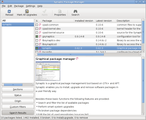
\includegraphics[width=.8\textwidth]{Figures/synaptic.png}
\caption{Captura de tela do synaptic}
\label{fig:synaptic}
\end{figure}

\subsection{Ubuntu Software Center}

\index{Software Center}
\index{AppCenter}
Ferramenta inicialmente denominada \textit{AppCenter}, foi projetada
com o intuito de centralizar as atividades relativas � instala��o de
aplicativos em sistemas Ubuntu (navega��o pelo reposit�rio, instala��o e
remo��o de pacotes). Foi desenvolvido com base no \textit{gnome-app-install},
sendo escrito em Python e usa GTK+ como biblioteca gr�fica. Serve como
interface para o \textit{APT}, dado que o sistema de empacotamento desta
distribui��o � herdado do Debian.

\begin{figure}[h!]
\centering
  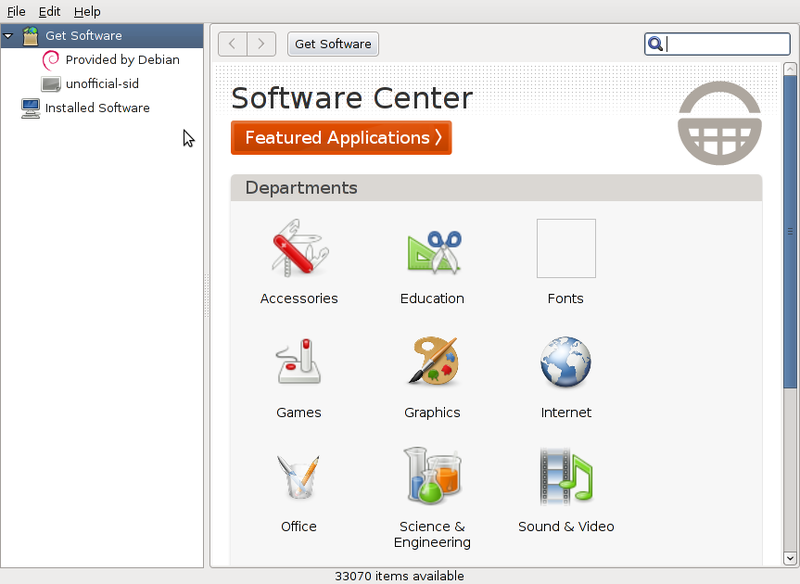
\includegraphics[width=.8\textwidth]{Figures/software-center.png}
\caption{Captura de tela do software-center}
\label{fig:software_center}
\end{figure}

%\subsection{AppNR}
%
%O \textit{AppNR}\footnote{\url{http://appnr.com/}} � um servi�o web que prov� uma
%interface para os reposit�rios de aplicativos da distribui��o Ubuntu. Al�m de
%navegar pelo reposit�rio e visualizar detalhes dos aplicativos, o usu�rio pode
%instalar pacotes, caso o seu navegador ofere�a suporte ao protocolo
%\textit{AptURL}.
%
%\begin{figure}[h!]
%\centering
%  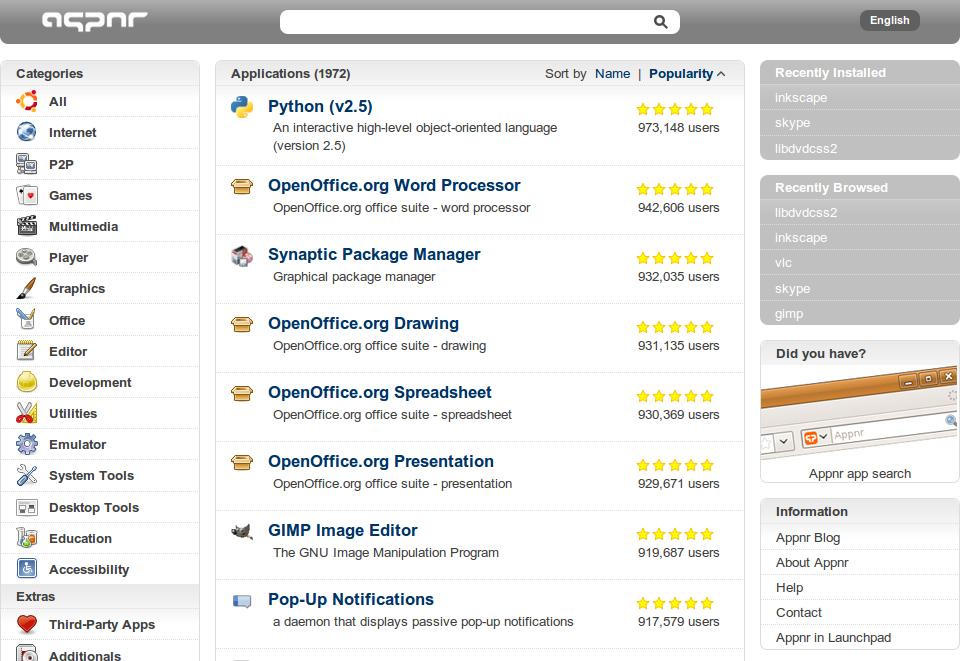
\includegraphics[width=.8\textwidth]{Figures/appnr-current.png}
%\caption{Captura de tela do \textit{AppNR}}
%\label{fig:software_center}
%\end{figure}

\section{Sele��o de programas}

O conjunto de programas instalados num determinado sistema � tipicamente
resultado de dois processos de sele��o: o primeiro � realizado no �mbito do
desenvolvimento da distribui��o e o segundo faz parte da manuten��o cotidiana
do sistema, realizado pelo usu�rio e/ou administrador da m�quina.

A sele��o e configura��o dos aplicativos b�sicos de uma distribui��o
(instalados por padr�o) s�o de responsabilidade da equipe que a desenvolve, com
diferentes n�veis de interfer�ncia da comunidade. Este � um ponto bastante
sens�vel nos projetos, dado que � um dos fatores que influenciam a escolha dos
usu�rios finais por qual distribui��o adotar, e pode revelar eventuais
conflitos de interesses. Por exemplo, a decis�o da Canonical que determinou,
sem debates p�blicos, a substitui��o do popular gerenciador de janelas GNOME
por um outro menos maduro, exp�s um modelo em que a comunidade e mesmo os
desenvolvedores envolvidos exercem papel limitado nos rumos do projeto
\cite{Paul:10}.

Por outro lado, ap�s a configura��o de um sistema b�sico, este � geralmente
personalizado para atender �s demandas espec�ficas dos usu�rios finais, por
meio da instala��o de programas adicionais. Ainda que a infraestrutura de
instala��o de softwares provida pelas distribui��es (geralmente baseada em
pacotes) simplifique a manuten��o de sistemas \cite{Cosmo:08}, a sele��o dos
programas inevitavelmente depender� de uma a��o humana. Com o desenvolvimento
deste trabalho pretende-se auxiliar o indiv�duo nesta tarefa, especialmente no
cen�rio em que o usu�rio n�o � dotado de experi�ncia pessoal e habilidade
suficientes para decidir qual aplicativo instalar.

\chapter{Sistemas Recomendadores} \label{chapter:recomendadores}

%A populariza��o de recursos computacionais e do acesso � Internet nas
%�ltimas d�cadas proporcionou um aumento expressivo na diversidade de servi�os e
%conte�do � disposi��o dos usu�rios. Um dos fatores para este aumento � que
%os usu�rios, que anteriormente eram considerados meros consumidores,
%apresentam-se atualmente como produtores de conte�do. \cite{Castells:06} analisa
%este fen�meno e afirma que a maioria da popula��o acredita que pode influenciar
%outras pessoas atuando no mundo atrav�s da sua for�a de vontade e
%utilizando seus pr�prios meios. Isto pode ser observado no surgimento e
%prolifera��o de servi�os criados e mantidos pelos usu�rios: blogs, enciclop�dias
%colaborativas, como a Wikipedia\footnote{\url{http://wikipedia.org}},
%reposit�rios para compartilhamento de fotografia e v�deo, como Flickr
%\footnote{\url{http://flickr.com}} e Youtube\footnote{\url{http://youtube.com}},
%entre outros. Considerando a produ��o em termos de software, observa-se o
%exemplo das comunidades de software livre e/ou de c�digo aberto
%(FOSS\footnote{Termo consolidado no idioma ingl�s, acr�nimo para
%\textit{Free/Open-Source Software}, que diz respeito aos programas licenciados
%livremente para garantir aos usu�rios o direito de uso, estudo e modifica��o,
%por meio da disponibilidade do seu c�digo-fonte.}), que propiciam a constru��o
%coletiva de uma ampla gama de softwares de qualidade em constante atualiza��o
%e evolu��o, organizados na forma de um rossio \cite{Simon:08}.

Segundo \cite{Resnick:97}, os sistemas de recomenda��o aumentam a capacidade e
efic�cia de um processo de indica��o bastante popular nas rela��es sociais.
Existem recomenda��es produzidas exclusivamente por especialistas, a exemplo de
indica��es de filmes publicadas nos principais jornais e revistas do pa�s por
cr�ticos de arte. Nos �ltimos anos, por�m, a opini�o e o comportamento de
usu�rios n�o especializados passaram a ser considerados nas recomenda��es, por
agregarem valor �s mesmas. O que acontece de forma expl�cita, quando o
pr�prio usu�rio escreve sua opini�o ou avalia a qualidade de um item, ou
impl�cita, quando suas prefer�ncias, comportamentos e transa��es s�o analisados
e incorporados � recomenda��o de forma transparente ao usu�rio.

O problema da recomenda��o � comumente formalizado atrav�s de uma estrutura de
pontua��o como representa��o computacional da utilidade dos itens para os
usu�rios ou clientes. A partir de avalia��es feitas pelos pr�prios usu�rios do
sistema, tenta-se estimar pontua��es para os itens que ainda n�o foram
avaliados pelos mesmos. Uma vez que esta estimativa tenha sido feita, pode-se
recomendar os itens com maior pontua��o estimada.

O conceito de utilidade, por�m, � subjetivo e arduamente mensur�vel devido �s
dificuldades em distinguir qualitativamente e definir quantitativamente os
fatores que a determinam. Portanto, com a ressalva de que estas medidas n�o
representam necessariamente a realidade, as pontua��es s�o usadas como
aproxima��es, pois t�m como base as avalia��es registradas pelos pr�prios usu�rios.

\section{A��es} \label{sec:acoes}

Sistemas de recomenda��o s�o implementados nos mais diversos contextos
e podem ser projetados com finalidades distintas. Abaixo est�o descritas
algumas a��es relacionadas a estes sistemas identificadas por
\cite{Herlocker:04}.

\begin{description}

\item[Anota��o em contexto.] Os primeiros sistemas de recomenda��o eram
  utilizados num cen�rio de informa��o estruturada (mensagens classificadas
  num contexto), e auxiliavam os usu�rios a selecionarem as mensagens a serem
  lidas dentro de cada contexto.

\item[Encontrar itens relevantes.] O sistema sugere itens para o usu�rio
  atrav�s de uma lista ordenada de forma decrescente, de acordo com a
  probabilidade do item ser considerado relevante pelo usu�rio. Esta � a a��o
  mais comum entre os sistemas de recomenda��o comerciais, atraindo grande
  parte das pesquisas relacionadas com o tema.

\item[Encontrar todos os itens relevantes.] Em situa��es em que n�o se deseja
  ignorar nenhum item relevante, ao inv�s da recomenda��o de apenas alguns,
  todos os itens considerados relevantes devem ser retornados.

\item[Sequ�ncia recomendada.] Quando n�o somente os itens recomendados importa,
  mas tamb�m a ordem em que eles s�o apresentados, caracteriza-se a a��o de
  recomenda��o de sequ�ncia.

\item[Express�o de opini�o.] A recomenda��o em si muitas vezes n�o � o que
  atrai usu�rios desses sistemas. Alguns est�o interessados simplesmente em
  emitir suas opini�es. Esta a��o � comum em ambientes que disponibilizam um
  espa�o para os usu�rios registrarem seus coment�rios e avalia��es sobre os
  produtos.

\item[Ajudar usu�rios.] Alguns usu�rios utilizam sistemas de recomenda��o
  por acreditarem que a comunidade se beneficia da sua contribui��o. Apesar de
  nem sempre aparecerem juntas, tal atividade est� comumente relacionada com a
  express�o de opini�o.

\item[Navega��o.] Alguns usu�rios utilizam recomendadores mesmo quando n�o t�m
  planos de consumir produto algum, apenas para navegar entre os itens
  dispon�veis. Neste caso, aspectos como a interface, facilidade de uso e
  natureza da informa��o provida s�o de extrema import�ncia.

\end{description}

\section{Desafios}

O desenvolvimento de sistemas recomendadores t�m como desafios quest�es
inerentes ao problema de recomenda��o e sua representa��o computacional. As
estrat�gias e t�cnicas propostas devem levar em conta tais quest�es e tentar
contorn�-las na medida do poss�vel. Alguns destas quest�es foram apontadas
por \cite{Vozalis:03} e s�o citadas a seguir.

\begin{description}

  \item[Qualidade das recomenda��es.] Usu�rios esperam recomenda��es nas
    quais eles possam confiar. Esta confiabilidade � alcan�ada na medida em
    que se diminui a incid�ncia de falsos positivos, em outras palavras,
    recomenda��es que n�o interessam ao usu�rio;

  \item[Esparsidade.] A exist�ncia de poucas rela��es usu�rio-item resulta
     numa matriz de relacionamentos esparsa, o que dificulta a localiza��o de
     usu�rios com prefer�ncias semelhantes (rela��es de vizinhan�a) e
     resulta em recomenda��es fracas.

  \item[Escalabilidade.] A complexidade do c�lculo de recomenda��es cresce
    tanto com o n�mero de clientes quanto com a quantidade de itens,
    portanto a escalabilidade dos algoritmos � um ponto importante a ser
    considerado.

  \item[Transitividade de vizinhan�a.] Usu�rios que t�m comportamento
    semelhante a um determinado usu�rio n�o necessariamente t�m
    comportamento semelhante entre si. A captura deste tipo de rela��o pode ser
    desej�vel mas em geral esta informa��o n�o � resguardada, exigindo a
    aplica��o de m�todos espec�ficos para tal.

  \item[Sin�nimos.] Quando o universo de itens possibilita a exist�ncia
    de sin�nimos, a solu��o deve levar esta informa��o em conta para prover
    melhores resultados.

  \item[Primeira avalia��o.] Um item s� pode ser recomendado se ele tiver sido
    escolhido por um usu�rio anteriormente. Portanto, novos itens precisam ter
    um tratamento especial at� que sua presen�a seja ``notada''.

  \item[Usu�rio incomum.] Indiv�duos com opini�es que fogem do usual, que n�o
    concordam nem discordam consistentemente com nenhum grupo, normalmente n�o
    se beneficiam de sistemas de recomenda��es.

\end{description}

%FIXME [Desenvolver os temas: perfis de usuario e privacidade]

%\subsection{Perfis de Usu�rio}
%. Identidade\\
%. Gera��o e manuten��o de perfil\\
%. Reputa��o
%
%\subsection{Privacidade}

%FIXME [Analisar complexidade de cada tecnica]
%FIXME [Produzir figuras ilustrativas do naive bayes]
\subsection{T�cnicas} \label{sec:tecnicas}

O desenvolvimento de sistemas de recomenda��o tem suas ra�zes em �reas
distintas e o problema computacional a ser tratado est� fortemente relacionado
com outros problemas cl�ssicos, como classifica��o e recupera��o de informa��o
em documentos de texto.

A fim de obter a informa��o desejada, o usu�rio de uma ferramenta de busca
deve traduzir suas necessidades de informa��o para uma consulta
(\textit{query}, em ingl�s), que geralmente � representada por um conjunto de
\textit{palavras-chave}. O desafio do buscador � recuperar os documentos da
cole��o que s�o relevantes para a consulta, baseando-se nos termos que a
constituem.  Ademais, visto que a busca pode retornar um n�mero excessivo de
documentos, � desej�vel que este resultado seja apresentado ao usu�rio em ordem
decrescente de relev�ncia, aumentando assim as chances de a informa��o desejada
ser encontrada com rapidez. Para tanto, cada documento da cole��o deve ter uma
pontua��o (peso) que indique seu grau de import�ncia para a referida
\textit{query}. Tra�ando um paralelo com o problema de recomenda��o, a
identidade e/ou o comportamento do usu�rio representaria a consulta ao sistema
de busca, que provocaria o retorno dos itens de maior peso, ou seja, com maior
potencial de aceita��o pelo usu�rio.

Na busca por informa��o, assume-se que as necessidades do usu�rio s�o
particulares e passageiras, e por isso a reincid�ncia de \textit{queries} n�o �
muito frequente \cite{Manning:09}. Por�m, em situa��es onde se observa que as
mesmas consultas s�o aplicadas com uma certa frequ�ncia, � interessante que o
sistema suporte consultas permanentes. Desta forma a computa��o necess�ria pode
ser realizada previamente e apresentada sempre que a consulta for requisitada.
Se a classe de documentos que satisfazem a uma dessas \textit{queries}
permanentes � tida como uma categoria, o processo de realiza��o das consultas
pr�vias pode ser caracterizado como uma classifica��o. O problema da
classifica��o diz respeito � determina��o de relacionamentos entre um dado
objeto e um conjunto de classes pr�-definidas.

A recomenda��o pode ser vista como uma classifica��o, na qual os itens s�o
categorizados entre duas classes: relevantes e irrelevantes -- os relevantes
seriam recomendados. Por�m, a defini��o de consultas ou regras fixas para uma
busca n�o � uma estrat�gia eficiente neste caso, porque a consulta estaria
diretamente relacionada com a identidade do usu�rio e portanto deveria ser
escrita especialmente para ele.

Todavia, a disciplina de intelig�ncia artificial aborda a quest�o da
classifica��o atrav�s de estrat�gias que n�o se baseiam em busca. Algoritmos
de aprendizado de m�quina s�o utilizados para a constru��o de modelos de
classifica��o ``inteligentes'', que ``aprendem'' atrav�s da an�lise de
exemplos. Os m�todos supervisionados fundamentam-se na constru��o de um
classificador que aprende na medida em que lhe s�o apontados exemplos de
objetos classificados. S�o caracterizados como supervisionados porque as
classes atribu�das aos objetos de treinamento s�o determinadas por um ser
humano, que atua como um supervisor orientando o processo de aprendizado
\cite{Manning:09}. Por outro lado, algoritmos n�o supervisionados procuram
identificar padr�es de organiza��o nos dados sem que haja uma classifica��o
pr�via dos exemplos.

A seguir s�o apresentadas algumas t�cnicas para tratamento destes problemas
que tamb�m s�o utilizadas na constru��o de sistemas de recomenda��o, dando
suporte �s estrat�gias apresentadas na se��o \ref{sec:estrategias}.

\subsubsection{K-NN} \label{sec:knn}

\textit{K-nearest neighbors (k-NN)}, em portugu�s \textit{k vizinhos mais
pr�ximos}, � mais um algoritmo de aprendizado supervisionado para
classifica��o. Este m�todo baseia-se no conceito de vizinhan�a, que representa
um conjunto de objetos que est�o pr�ximos no espa�o de busca.

O \textit{K-NN} n�o exige nenhum treinamento pr�vio com os dados de exemplo,
que podem ser diretamente armazenados como vetores de atributos acompanhados
por suas devidas classes. A classifica��o de um novo objeto parte do c�lculo da
vizinhan�a do mesmo, que � composta por $k$ objetos.

A determina��o da vizinhan�a est� diretamente relacionada com o conceito de
proximidade entre objetos, que pode ser expressa em termos de similaridade ou
de dist�ncia entre os mesmos (quanto maior a dist�ncia, menor a similaridade).
Existem diversas medidas para mensurar estes conceitos, deve-se adotar a
m�trica que melhor se adeque ao dom�nio da aplica��o e conjunto de dados.
A tabela \ref{tab:knn_distancia} apresenta algumas dessas medidas, onde os
objetos $X$ e $Y$ s�o representados por seus vetores $\vec{X} = (x_1,...,x_n)$
e $\vec{Y} = (y_1,...,y_n)$. A similaridade de cosseno mede a similaridade de
dois vetores atrav�s do cosseno do �ngulo entre os mesmos. O coeficiente de
\textit{Pearson} � equivalente ao cosseno do �ngulo entre os vetores
centralizados na m�dia. E o coeficiente de \textit{Tanimoto} � uma extens�o da
similaridade de cossenos que resulta no �ndice de \textit{Jaccard} para
atributos bin�rios.

\begin{table}[h!]
  \caption{K-NN: Medidas de dist�ncia e similaridade entre objetos}
  \label{tab:knn_distancia}
  \centering
  \newcommand\T{\rule{0pt}{2.8ex}}
  \newcommand\B{\rule[-1.8ex]{0pt}{0pt}}
  \begin{tabular}{| l | l |}
    \hline
    Dist�ncia euclidiana &
    \T\B$\mathid{D}(X,Y) = \sqrt{(x_1-y_1)^2+(x_2-y_2)^2+...+(x_n-y_n)^2}$\\
    \hline
    Similaridade de cosseno &
    $\mathid{sim}(X,Y) = \frac{\T\vec{X} \cdot \vec{Y}}{|\vec{X}| |\vec{Y}|}
                       = \frac{\textstyle \sum_{1\leq i \leq n} x_i y_i}
                              {\textstyle \sqrt{\sum_{1\leq i \leq n} x_i^2}
                               \sqrt{\sum_{1\leq i \leq n} y_i^2}\B}$\\
    \hline
    Coeficiente de \textit{Pearson} &
    $\mathid{P}(X,Y) = \frac{\T\textstyle\sum_{1 \leq i \leq n} (x_i-\bar{x})
                                     (y_i-\bar{y})}
                   {\textstyle\sqrt{\sum_{1 \leq i \leq n} (x_i-\bar{x})^2}
                    \sqrt{\sum_{1 \leq i \leq n} (y_i-\bar{y})^2}\B}$\\
    \hline
    Coeficiente de \textit{Tanimoto} &
    $\mathid{T}(X,Y) = \frac{\T\textstyle\vec{X} \cdot \vec{Y}}
                            {\textstyle |\vec{X}|^2 + |\vec{Y}|^2 -
                             \vec{X} \cdot \vec{Y}}$\\
    \hline
  \end{tabular}
\end{table}

Ap�s a defini��o de vizinhan�a, a classe mais frequente entre seus $k$ vizinhos
� atribu�da ao novo objeto. Desta forma, a similaridade tamb�m pode ser
entendida como grau de influ�ncia entre os objetos. Os objetos mais semelhantes
a um novo objeto ter�o maior influ�ncia no c�lculo de sua classifica��o.

\newpage
%\vspace{0.3cm}
\hspace{-1.4cm}
\textbf{Sele��o de atributos} \label{sec:selecao_atributos}

Uma grande quantidade de atributos a ser considerada resulta em alta
complexidade computacional, al�m de geralmente mascarar a presen�a de ru�dos
(dados que prejudicam a acur�cia da classifica��o quando considerados).
A fim de amenizar este problema, � comum a realiza��o de um processo denominado
sele��o de atributos, que consiste em escolher alguns atributos dos dados e
utilizar apenas estes como conjunto de treinamento para a classifica��o. Esta
sele��o equivale � substitui��o de um classificador complexo por um mais
simples. \cite{Manning:09} defende que, especialmente quando a quantidade de
dados de treinamento � limitada, modelos mais fracos s�o prefer�veis.

A sele��o de atributos geralmente � realizada para cada classe em separado,
seguida pela combina��o dos diversos conjuntos. Abaixo s�o apresentados alguns
m�todos de escolha.

\begin{description}

  \item[Informa��o m�tua.] An�lise de quanto a presen�a ou aus�ncia de um
    atributo contribui para a tomada de decis�o correta por uma determinada
    classe. Informa��o m�tua m�xima significa que o atributo � um indicador
    perfeito para pertencimento a uma classe. Isto acontece quando um objeto
    apresenta o atributo se e somente se o objeto pertence � classe;

  \item[Independ�ncia de eventos.] Aplica��o do teste estat�stico $\chi^2$ para
    avaliar a independ�ncia de dois eventos -- neste caso, um atributo e uma
    classe. Se os dois eventos s�o dependentes, ent�o a ocorr�ncia do atributo
    torna a ocorr�ncia da classe mais prov�vel.

  \item[Baseado em frequ�ncia.] Sele��o dos atributos mais comuns para uma
    classe.

\end{description}

Os m�todos apresentados acima s�o ``gulosos'', ou seja, assumem escolhas �timas
locais na esperan�a de serem �timas globais. Como resultado, podem selecionar
atributos que n�o acrescentam nenhuma informa��o para a classifica��o quando
considerados outros previamente escolhidos. Apesar disto, algoritmos n�o
gulosos s�o raramente utilizados devido a seu custo computacional
\cite{Manning:09}.

\subsection{Classificador bayesiano}

\textit{Bayes ing�nuo} � uma solu��o para classifica��o que figura entre os
algoritmos de aprendizado de m�quina supervisionados. O classificador apoia-se
num modelo probabil�stico que aplica o teorema de Bayes com fortes suposi��es
de independ�ncia de atributos -- por esta raz�o o m�todo � considerado ing�nuo.
Em outras palavras, a presen�a ou aus�ncia de um atributo em um objeto de uma
classe n�o estaria relacionada com a incid�ncia de nenhum outro atributo.

A decis�o acerca da classe a qual um objeto pertence � tomada de acordo com o
modelo de probabilidade m�xima posterior \textit{(MAP)}, indicada na equa��o
\ref{eq:map}. Dado que $C$ � o conjunto de classes e $x$ objeto a ser
classificado, a classe atribu�da a este ser� a que apresentar maior
probabilidade condicionada a $x$. $\hat{P}$ � utilizado ao inv�s de $P$ porque
geralmente n�o se sabe o valor exato das probabilidades, que s�o estimadas a
partir dos dados de treinamento.

\begin{equation}
\label{eq:map}
  \mathid{c_{MAP}} = \underset{c \in C}{\operatorname{arg\ max}} \ \hat{P}(c|x)
\end{equation}

A equa��o \ref{eq:bayes} aplica o Teorema de Bayes para probabilidades
condicionadas. Na pr�tica, apenas o numerador da fra��o interessa, visto que o
denominador � constante para todas as classes, portanto n�o afeta o
$\operatorname{arg\ max}$ (equa��o \ref{eq:bayes_no_deno}).

\begin{eqnarray}
\label{eq:bayes}
  \mathid{c_{MAP}} & = & \underset{c \in C}{\operatorname{arg\ max}} \
                         \frac{\hat{P}(x|c) \hat{P}(c)}{\cancel{\hat{P}(x)}} \\
                {} & {} & {} \nonumber \\
\label{eq:bayes_no_deno}
                   & = & \underset{c \in C}{\operatorname{arg\ max}} \
                         \hat{P}(x|c) \hat{P}(c)
\end{eqnarray}

� neste ponto que a independ�ncia de atributos � importante. Considera-se que
um documento $x$ pode ser caracterizado por uma s�rie de atributos $x_i$ -- no
caso de documentos de texto, os atributos s�o os pr�prios termos. Assumindo que
a ocorr�ncia de atributos acontece independentemente, tem-se que:

\begin{equation}
\label{eq:independencia}
  \hat{P}(x|c) = \hat{P}(x_1,x_2,...,x_n|c)
               = \hat{P}(x_1|c) \hat{P}(x_2|c)\ ...\ \hat{P}(x_n|c)
\end{equation}

Portanto, a fun��o de decis�o pode ser reescrita atrav�s da equa��o
\ref{eq:bayes_prod}. Cada par�metro condicional $\hat{P}(x_i|c)$ � um peso
que representa a qualidade do atributo $x_i$ como indicador da classe $c$,
enquanto que $\hat{P}(c)$ � a frequ�ncia relativa da classe $c$.

\begin{equation}
\label{eq:bayes_prod}
  \mathid{c_{MAP}} = \underset{c \in C}{\operatorname{arg\ max}} \ \
                     \hat{P}(c) \prod_{1 \le i \le n} \hat{P}(x_i|c)
\end{equation}

Os par�metros s�o obtidos atrav�s da estimativa de maior probabilidade
\textit{(MLE)}, que corresponde ao valor mais prov�vel de cada par�metro de
acordo com os dados de treinamento. A equa��o \ref{eq:p_c} traz a estimativa de
$\hat{P}(c)$, onde $N_c$ � o n�mero de objetos da classe $c$ e $N$ � o n�mero
total de documentos.

\begin{equation}
\label{eq:p_c}
  \hat{P}(c) = \frac{N_c}{N}
\end{equation}

As probabilidades condicionais s�o estimadas como a frequ�ncia relativa do
atributo $x$ em objetos que pertencem � classe $c$. Na equa��o \ref{eq:p_xc},
$T_{\mathit{cx}}$ � o n�mero de ocorr�ncias de $x$ em objetos de exemplo da
classe $c$ e $V$ � o conjunto de atributos que os objetos podem apresentar.

\begin{equation}
\label{eq:p_xc}
  \hat{P}(x|c) = \frac{T_{\mathit{cx}}}
                      {\displaystyle \sum_{x' \in V} T_{\mathit{cx}'}}
\end{equation}

No entanto, a estimativa \textit{MLE} � zero para combina��es atributo-classe
que n�o ocorrem nos dados de treinamento. Considerando que as probabilidades
condicionais de todos os atributos ser�o multiplicadas (equa��o
\ref{eq:bayes_prod}), a simples ocorr�ncia de uma probabilidade zerada resulta
na desconsidera��o da classe na referida classifica��o. E de fato, dados de
treinamento nunca s�o abrangentes o suficiente para representar a frequ�ncia de
eventos raros de forma adequada \cite{Manning:09}. Para eliminar
$\mathit{zeros}$, adiciona-se $1$ a cada termo da equa��o \ref{eq:p_xc}:

\begin{equation}
\label{eq:p_xc+1}
  \hat{P}(x|c) = \frac{T_{\mathit{cx}}+1}
                      {\displaystyle \sum_{x' \in V} T_{\mathit{cx}'}+1}
\end{equation}

O classificador bayesiano tamb�m � sens�vel a ru�dos, logo, sua performance �
igualmente beneficiada pelo processo de sele��o de atributos descrito na se��o
\ref{sec:selecao_atributos}.

Apesar de a independ�ncia de atributos n�o ser verificada para a maioria
dos dom�nios de aplica��o, na pr�tica o Bayes ing�nuo apresenta resultados
satisfat�rios. \cite{Zhang:04} atribui a surpreendente boa performance deste
m�todo ao fato de que a mera exist�ncia de depend�ncias entre atributos n�o
prejudicaria a classifica��o, mas sim o modo como as depend�ncias est�o
distribu�das ao longo das classes. Segundo o autor, desde que as depend�ncias
estejam distribu�das igualmente nas classes, n�o h� problema em haver
depend�ncia forte entre dois atributos.

\vspace{0.3cm} \hspace{-1.4cm}
\textbf{Variantes do modelo Bayes ing�nuo}

As duas principais variantes de implementa��o do classificador bayesiano,
denominadas de modelo \textit{multinomial} e de \textit{Bernoulli}, diferem
fundamentalmente na maneira como os objetos s�o representados.

O primeiro modelo utiliza uma representa��o que considera informa��es espaciais
sobre o objeto. Na classifica��o de documentos de texto, por exemplo, o modelo
gera um atributo para cada posi��o do documento, que corresponde a um termo do
vocabul�rio. J� o modelo de \textit{Bernoulli} produz um indicador de
presen�a ou aus�ncia para cada poss�vel atributo (no caso de texto, cada termo
do vocabul�rio).

A escolha da representa��o de documentos adequada � uma decis�o cr�tica no
projeto de um classificador, visto que o pr�prio significado de um atributo
depende da representa��o. No \textit{multinomial}, um atributo pode assumir
como valor qualquer termo do vocabul�rio, o que resulta numa representa��o do
documento correspondente � sequ�ncia de termos do mesmo. J� para o modelo de
\textit{Bernoulli}, um atributo pode assumir apenas os valores $0$ e $1$, e a
representa��o do documento � uma sequ�ncia de $0$s e $1$s do tamanho do
vocabul�rio.

%A figura \ref{fig:exemplo_bayes} ilustra as peculiaridades de cada
%representa��o.
%
%\begin{figure}[ht]
%\centering
%\begin{tabular}{*4{c}}
%\begin{overpic}[width=2.3cm]{fig/doc_background.png}\put(60,5){\scriptsize (1)}
%  \put(5,44){\parbox{1.8cm}{\scriptsize Por motivo \\ de seguran�a, \\
%    comunicamos a todos os clientes que atualizem sua senha por email.}}
%    \end{overpic} &
%\begin{overpic}[width=2.3cm]{fig/doc_background.png}\put(60,5){\scriptsize (2)}
%  \put(5,44){\parbox{1.8cm}{\scriptsize Atualiza��o \\ urgente de \\  senha.
%    \\ \\ Clique aqui.}}\end{overpic} &
%\begin{overpic}[width=2.3cm]{fig/doc_background.png}\put(60,5){\scriptsize (3)}
%  \put(5,44){\parbox{1.8cm}{\scriptsize Voc� foi \\ sorteado e \\ acaba de
%    ganhar 1 milh�o de reais. Clique aqui e saiba como resgatar seu pr�mio.}}
%    \end{overpic} &
%\begin{overpic}[width=2.3cm]{fig/doc_background.png}\put(60,5){\scriptsize (4)}
%  \put(5,44){\parbox{1.8cm}{\scriptsize Perca peso f�cil e de forma divertida.
%    Pare de sofrer!}}\end{overpic} \\
%\begin{overpic}[width=2.3cm]{fig/doc_background.png}\put(60,5){\scriptsize (5)}
%  \put(5,44){\parbox{1.8cm}{\scriptsize Emagre�a 10kg em duas semanas! Clique
%    aqui e descubra como.}}\end{overpic} &
%\begin{overpic}[width=2.3cm]{fig/doc_background.png}\put(60,5){\scriptsize (6)}
%  \put(5,44){\parbox{1.8cm}{\scriptsize Compre viagra com 69\% de desconto!}}
%    \end{overpic} &
%\begin{overpic}[width=2.3cm]{fig/doc_background.png}\put(60,5){\scriptsize (7)}
%  \put(5,44){\parbox{1.8cm}{\scriptsize Se voc� n�o pode mudar sua vida, mude
%    pelo menos a sua bolsa!}}\end{overpic} &
%\begin{overpic}[width=2.3cm]{fig/doc_background.png}\put(60,5){\scriptsize (8)}
%  \put(5,44){\parbox{1.8cm}{\scriptsize Aprenda a investir na bolsa em uma
%    semana.}}\end{overpic}
%\end{tabular}
%\caption{Cole��o de documentos classificados em \textit{spam} e \textit{n�o-spam}}
%\label{fig:colecao_spam}
%\end{figure}

\subsection{Medida $\boldsymbol{\tfidf}$}

Acr�nimo para \textit{term frequency - inverse document frequency}, $\tfidf$ �
uma medida de peso cl�ssica utilizada em ferramentas de busca em texto para
ordena��o do resultado da consulta pela relev�ncia dos documentos.

O universo da busca � uma cole��o de documentos de texto. Um documento por sua
vez � uma cole��o de palavras, geralmente referenciadas como \textit{termos do
documento}. O conjunto de todas as palavras presentes nos documentos da
cole��o � denominado \textit{dicion�rio} ou \textit{vocabul�rio}. Desta forma,
um documento $d$ composto por $n$ termos do vocabul�rio $V$ pode ser
representado como $d = \{t_1, t_2, ..., t_n | 1 \leq i \leq n, t_i \in V\}$.

Contudo, alguns termos do vocabul�rio, designados como \textit{stop words}, s�o
normalmente desconsiderados no c�lculo de relev�ncia dos documentos por serem
muito frequentes na cole��o e, em decorr�ncia disto, pouco informativos acerca
do teor dos textos. Artigos e pronomes, por exemplo, geralmente figuram nesta
categoria.

Outra considera��o acerca da representa��o dos documentos como conjuntos de
termos � a realiza��o de normaliza��es morfol�gicas. Diferentes palavras que
dizem respeito ao mesmo conceito podem ser utilizadas ao longo de uma cole��o,
por exemplo, os termos \textit{casa}, \textit{casinha} e \textit{casas}. Em
certos contextos, deseja-se que a busca por uma determinada variante retorne
ocorr�ncias de todas as outras possibilidades. Neste caso, os termos devem ser
tratados em sua forma normalizada, eliminando varia��es como plurais e flex�es
verbais. Os processos mais comuns de normaliza��o s�o: \textit{stemming}, que
reduz a palavra ao seu radical; e \textit{lematiza��o}, que reduz a palavra �
sua forma can�nica (por exemplo, verbos no infinitivo, substantivos no singular
masculino etc). A figura \ref{fig:normalizacao} apresenta um documento de texto
numa cole��o hipot�tica\footnote{Os textos utilizados nos exemplos desta se��o
s�o excertos de letras de m�sica de diversos compositores brasileiros.} e a sua
representa��o ap�s elimina��o de \textit{stop words} e procedimento de
\textit{stemming}.

\begin{figure}[ht]
\centering
\begin{tabular}{*3{c}}
\begin{overpic}[width=2.8cm]{Figures/doc_background.png}
  \put(12,44){\parbox{1.8cm}{\scriptsize August\sout{a}, gra�\sout{as} \sout{a}
    deus, entr\sout{e} \sout{voc�} \sout{e} \sout{a} Ang�l\sout{ica},
    \sout{eu} encontr\sout{ei} \sout{a} Consol\sout{a��o}, \sout{que}
    v\sout{eio} olh\sout{ar} \sout{por} \sout{mim} \sout{e} \sout{me}
    d\sout{eu} \sout{a} m�o.}}\end{overpic}  &
\raisebox{1.5cm}{\Huge $\Longrightarrow$} &
\begin{overpic}[width=2.8cm]{Figures/doc_background.png}
  \put(12,44){\parbox{1.8cm}{\scriptsize august \ \ \ grac \\ deus entr angel
    encontr consol v\ \ \  olh\ \ \  d\ \ \  m�o}}\end{overpic}
\end{tabular}
\caption{Elimina��o de \textit{stop words} e normaliza��o do documento por
         \textit{stemming}}
\label{fig:normalizacao}
\end{figure}

A simples presen�a de um termo da \textit{query} em um documento da cole��o j�
� um indicativo de que o mesmo tem alguma rela��o com a consulta. No entanto, a
quantidade de vezes que o termo ocorre � ainda mais informativo sobre sua
rela��o com o conte�do do documento. Intuitivamente, os documentos que
referenciam os termos de uma \textit{query} com mais frequ�ncia est�o mais
fortemente relacionados com a mesma, e por isso deveriam receber uma maior
pontua��o de relev�ncia. O peso $\tf_{t,d}$ (\textit{term frequency})
quantifica esta no��o intuitiva, relacionando documentos da cole��o e termos do
dicion�rio de acordo com a frequ�ncia destes nos documentos. Em sua abordagem
mais simples, $\tf_{t,d}$ � igual ao n�mero de ocorr�ncias do termo $t$ no
documento $d$.

A figura \ref{fig:colecao} ilustra uma cole��o de documentos, cujos valores de
$\tf_{t,d}$ para alguns termos do dicion�rio s�o apresentados na tabela
\ref{tab:tf}. Por exemplo, a palavra \textit{morena} ocorre duas vezes
no documento $(1)$, por isso $\tf_{\mathit{moren},1} = 2$. O c�lculo do
$\tf$s j� considera os radicais dos termos, resultantes de um processo de
\textit{stemming}. Em raz�o disto, $\tf_{\mathit{olh},2} = 3$, pois tanto a
palavra \textit{olho} quanto as diferentes flex�es do verbo \textit{olhar}
contribuem para a contagem de frequ�ncia do termo \textit{olh}. Na tabela
\ref{tab:tf}, os radicais dos voc�bulos s�o seguidos por algumas varia��es, a
t�tulo de ilustra��o.

\begin{figure}[ht]
\centering
\begin{tabular}{*4{c}}
\begin{overpic}[width=2.3cm]{Figures/doc_background.png}\put(60,5){\scriptsize (1)}
  \put(5,44){\parbox{1.8cm}{\scriptsize Morena,\\ minha morena, tira a roupa da
    janela. Vendo a roupa sem a dona, eu penso na dona sem ela.}}\end{overpic} &
\begin{overpic}[width=2.3cm]{Figures/doc_background.png}\put(60,5){\scriptsize (2)}
  \put(5,44){\parbox{1.8cm}{\scriptsize Olha o \\ jeito dela, morena cor de
    canela, pode morrer de paix�o quem olhar nos olhos dela.}}\end{overpic} &
\begin{overpic}[width=2.3cm]{Figures/doc_background.png}\put(60,5){\scriptsize (3)}
  \put(5,44){\parbox{1.8cm}{\scriptsize O cravo brigou com a rosa debaixo de
    uma sacada. O cravo saiu ferido.}}\end{overpic} &
\begin{overpic}[width=2.3cm]{Figures/doc_background.png}\put(60,5){\scriptsize (4)}
  \put(5,44){\parbox{1.8cm}{\scriptsize Morena dos olhos d'�gua, tira os seus
    olhos do mar.}}\end{overpic} \\
\begin{overpic}[width=2.3cm]{Figures/doc_background.png}\put(60,5){\scriptsize (5)}
  \put(5,44){\parbox{1.8cm}{\scriptsize Queixo-me �s rosas, mas que bobagem,
    as rosas n�o falam.}}
    \end{overpic} &
\begin{overpic}[width=2.3cm]{Figures/doc_background.png}\put(60,5){\scriptsize (6)}
  \put(5,44){\parbox{1.8cm}{\scriptsize Morena de Angola que leva o chocalho
    amarrado na canela.}}\end{overpic} &
\begin{overpic}[width=2.3cm]{Figures/doc_background.png}\put(60,5){\scriptsize (7)}
  \put(5,44){\parbox{1.8cm}{\scriptsize Onde vais \\ morena Rosa, com essa rosa
    no cabelo e esse andar de mo�a prosa.}}\end{overpic} &
\begin{overpic}[width=2.3cm]{Figures/doc_background.png}\put(60,5){\scriptsize (8)}
  \put(5,44){\parbox{1.8cm}{\scriptsize A padaria Dona Morena vende p�o de
    cravo e canela.}}\end{overpic}
\end{tabular}
\caption{Cole��o de documentos}
\label{fig:colecao}
\end{figure}

\begin{table}[h!]
  \caption{Frequ�ncia dos termos nos documentos da cole��o}
  \label{tab:tf}
  \centering
  \small
  \begin{tabular}{| l | c | c | c | c | c | c | c | c |}
    \hline
    \multicolumn{9}{|c|}{$\boldsymbol{\tf_{t,d}}$}\\
    \hline
    \backslashbox{\textbf{\textit{Termo}}}{\vspace{-0.2cm}\textbf{\textit{Doc}}}&
    \textbf{(1)}&\textbf{(2)}&\textbf{(3)}&
    \textbf{(4)}&\textbf{(5)}&\textbf{(6)}&
    \textbf{(7)}&\textbf{(8)}\\
    \hline
    moren \textit{\{a,o\}} & $2$ & $1$ & $0$ & $1$ & $0$ & $1$ & $1$ & $1$ \\
    \hline
    roup \textit{\{a,�o\}} & $2$ & $0$ & $0$ & $0$ & $0$ & $0$ & $0$ & $0$ \\
    \hline
    don \textit{\{a,o\}} & $2$ & $0$ & $0$ & $0$ & $0$ & $0$ & $0$ & $1$ \\
    \hline
    crav \textit{\{o,eiro\}} & $0$ & $0$ & $2$ & $0$ & $0$ & $0$ & $0$ & $1$ \\
    \hline
    canel \textit{\{a,eira\}} & $0$ & $1$ & $0$ & $0$ & $0$ & $1$ & $0$ & $1$ \\
    \hline
    olh \textit{\{o,ar\}} & $0$ & $3$ & $0$ & $2$ & $0$ & $0$ & $0$ & $0$ \\
    \hline
    ros \textit{\{a,eira\}} & $0$ & $0$ & $1$ & $0$ & $2$ & $0$ & $2$ & $0$ \\
    \hline
    bob \textit{\{o,agem\}} & $0$ & $0$ & $0$ & $0$ & $1$ & $0$ & $0$ & $0$ \\
    \hline
  \end{tabular}
\end{table}

O conjunto de pesos determinado pelos $\tf$s dos termos de um documento
pode ser entendido como um resumo quantitativo do mesmo. Esta vis�o do
documento � comumente referenciada na literatura como ``saco de palavras'',
onde a disposi��o das palavras � ignorada e apenas a quantidade de ocorr�ncias
para cada termo � considerada.

Uma medida de relev�ncia baseada simplesmente na incid�ncia dos termos da
\textit{query} nos documentos ($\mathid{RI}$) poderia ser calculada atrav�s da
equa��o \ref{eq:relevancia_tf}.

\begin{equation}
\label{eq:relevancia_tf}
  \mathid{RI}_{d,q} = \sum_{t \in q} \tf_{t,d}
\end{equation}

No entanto, alguns termos t�m pouco poder de discrimina��o na determina��o
de relev�ncia de um documento, por estarem presentes em quase todos os
documentos. Ao passo que existem outros muito raros que quando presentes
s�o forte indicativo de relev�ncia. No contexto da cole��o da figura
\ref{fig:colecao}, por exemplo, a \textit{query} $\{\mathit{morena, bobagem}\}$
� composta por um termo muito frequente e outro muito raro. Coincidentemente,
os documentos $(3)$ e $(5)$, cont�m apenas um dos dois elementos da consulta,
por�m ambos apresentam $\tf_{t,d}=1$ para os respectivos termos. Todavia,
enquanto esta frequ�ncia se repete ao longo da cole��o m�ltiplas vezes para o
termo \textit{morena}, ela � �nica para o termo \textit{bobagem}, o que de fato
diferencia o documento $(5)$ dos demais.

O $\idf_t$ (\textit{inverse document frequency}) foi ent�o introduzido para
atenuar o efeito de termos muito comuns no c�lculo de relev�ncia, diminuindo o
peso relacionado a um termo por um fator que cresce com sua frequ�ncia em
documentos na cole��o \cite{Manning:09}. A equa��o \ref{eq:idf} apresenta a
forma cl�ssica do $\idf$, na qual $N$ representa o n�mero de documentos da
cole��o e $\df_t$ (\textit{document frequency}) � o n�mero de documentos que
cont�m o termo $t$. � comum que o universo da busca seja uma cole��o de
documentos de alt�ssima dimens�o, resultando em valores de $\df_t$ muito
discrepantes. O uso do $\log$ diminui a escala de valores, permitindo que
frequ�ncias muito grandes e muito pequenas sejam comparadas sem problemas.

\begin{equation}
\label{eq:idf}
\idf_t = \log \frac{N}{\df_t}
\end{equation}

Valores de $\idf_t$ para a cole��o da figura \ref{fig:colecao} s�o apresentados
na tabela \ref{tab:idf}. Novamente os radicais dos termos s�o considerados:
$\idf_\mathit{morena} = \idf_\mathit{moren} = \log \frac{8}{6} = 0.12$,
enquanto $\idf_\mathit{bobagem} = \idf_\mathit{bob} = \log \frac{8}{1} = 0.9$.

\begin{table}[h!]
  \caption{Valores de $\boldsymbol{\idf_t}$ para termos do dicion�rio}
  \label{tab:idf}
  \centering
  \small
  \begin{tabular}{| l | c | c | c | c | c | c | c | c |}
    \hline
    \textbf{\textit{Termo}} &
    moren & roup & don & crav & canel & olh & ros & bob\\
    \hline
    $\boldsymbol{\idf_t}$ &
    $0.12$ & $0.9$ & $0.6$ & $0.6$ & $0.42$ & $0.6$ & $0.42$ & $0.9$\\
    \hline
  \end{tabular}
\end{table}

A medida $\tfidf_{t,d}$ combina as defini��es de $\tf$ e $\idf$ (equa��o
\ref{eq:tfidf}), produzindo um peso composto com as seguintes propriedades:

\begin{enumerate}
  \item � alto quando $t$ ocorre muitas vezes em $d$ e em poucos documentos da
        cole��o (ambos $\tf$ e $\idf$ s�o altos);
  \item Diminui quando ocorre menos vezes em $d$ ($\tf$ mais baixo) ou em
        muitos documentos da cole��o ($\idf$ mais baixo);
  \item � muito baixa quando o termo ocorre em quase todos os documentos
        (mesmo para valores altos de $\tf$, para termos muito comuns o peso
        $\idf$ domina a f�rmula, em decorr�ncia do uso do $\log$).
\end{enumerate}

\begin{equation}
\label{eq:tfidf}
\tfidf_{t,d} = \tf_{t,d} \cdot \idf_t
\end{equation}

A medida de relev�ncia apresentada na equa��o \ref{eq:relevancia_tf} pode ser
refinada para somar os pesos $\tfidf$ do documento $d$ com rela��o aos termos
da \textit{query} $q$, resultando na media $\mathid{R}_{d,q}$ apresentada na equa��o
\ref{eq:relevancia} \cite{Manning:09}.

\begin{equation}
\label{eq:relevancia}
\mathid{R}_{d,q} = \sum_{t \in q} \tfidf_{t,d}
\end{equation}

A tabela \ref{tab:tfidf-resultado} apresenta a ordena��o dos documentos da
cole��o como resultado do c�lculo de relev�ncia por $\tfidf$ para as
consultas $q_1=\{\mathit{morena}\}$, $q_2=\{\mathit{morena, bobagem}\}$ e
$q_3=\{\mathit{morena, dona, rosa}\}$. Os valores $\tfidf_{t,d}$ foram
obtidos a partir da equa��o \ref{eq:tfidf}, com os pesos das tabelas
\ref{tab:tf} e \ref{tab:idf}. Por exemplo, $\tfidf_{\mathit{morena,1}} =
\tf_{\mathit{morena,1}} \cdot \idf_{\mathit{morena}} = 2 \cdot 0.12 = 0.24$.

\begin{table}[h!]
  \caption{Ordena��o dos documentos como resultado das consultas
           $\boldsymbol{q_1}$, $\boldsymbol{q_2}$ e $\boldsymbol{q_3}$}
  \label{tab:tfidf-resultado}
  \centering
  \footnotesize
  \begin{tabular}{| c | c | c | c | c | c | c | c | c | c | c | c | c | c |}
    \cline{1-3}\cline{5-8}\cline{10-14}
    \multirow{2}{*}{\textbf{doc}} & $\boldsymbol{q_1}$ & \multirow{2}{*}{$\boldsymbol{\mathsfsl{R}_{d,q}}$} & &
    \multirow{2}{*}{\textbf{doc}} & \multicolumn{2}{|c|}{$\boldsymbol{q_2}$} & \multirow{2}{*}{$\boldsymbol{\mathsfsl{R}_{d,q}}$} &&
    \multirow{2}{*}{\textbf{doc}} & \multicolumn{3}{|c|}{$\boldsymbol{q_3}$} & \multirow{2}{*}{$\boldsymbol{\mathsfsl{R}_{d,q}}$} \\
    \cline{2-2}\cline{6-7}\cline{11-13}
    & \textit{morena} & & & &
      \textit{morena} & \textit{bobagem} & & & &
      \textit{morena} &\textit{dona} & \textit{rosa} & \\
    \cline{1-3}\cline{5-8}\cline{10-14}
    (1) & $0.24$ & $0.24$ & &
    (5) & $0$ & $0.9$ & $0.9$ & &
    (1) & $0.24$ & $1.2$ & $0$ & $1.44$ \\
    \cline{1-3}\cline{5-8}\cline{10-14}
    (2) & $0.12$ & $0.12$ & &
    (1) & $0.24$ & $0$ & $0.24$ & &
    (8) & $0.12$ & $1.2$ & $0$ & $1.32$ \\
    \cline{1-3}\cline{5-8}\cline{10-14}
    (4) & $0.12$ & $0.12$ & &
    (2) & $0.12$ & $0$ & $0.12$ & &
    (7) & $0.12$ & $0$ & $0.84$ & $0.96$ \\
    \cline{1-3}\cline{5-8}\cline{10-14}
    (6) & $0.12$ & $0.12$ & &
    (4) & $0.12$ & $0$ & $0.12$ & &
    (5) & $0$ & $0$ & $0.84$ & $0.84$ \\
    \cline{1-3}\cline{5-8}\cline{10-14}
    (7) & $0.12$ & $0.12$ & &
    (6) & $0.12$ & $0$ & $0.12$ & &
    (3) & $0$ & $0$ & $0.42$ & $0.42$ \\
    \cline{1-3}\cline{5-8}\cline{10-14}
    (8) & $0.12$ & $0.12$ & &
    (7) & $0.12$ & $0$ & $0.12$ & &
    (2) & $0.12$ & $0$ & $0$ & $0.12$ \\
    \cline{1-3}\cline{5-8}\cline{10-14}
    (3) & $0$ & $0$ & &
    (8) & $0.12$ & $0$ & $0.12$ & &
    (4) & $0.12$ & $0$ & $0$ & $0.12$ \\
    \cline{1-3}\cline{5-8}\cline{10-14}
    (5) & $0$ & $0$ & &
    (3) & $0$ & $0$ & $0$ & &
    (6) & $0.12$ & $0$ & $0$ & $0.12$ \\
    \cline{1-3}\cline{5-8}\cline{10-14}
  \end{tabular}
\end{table}

Existem diversas variantes para o c�lculo dos pesos $\tf_{t,d}$ e $\idf_t$,
propostas com o intuito de aperfei�oar o processo de busca. Por exemplo,
geralmente a presen�a de uma palavra 20 vezes num documento n�o tem de fato
20 vezes mais representatividade do que uma ocorr�ncia �nica. Documentos
distintos podem referenciar o mesmo conceito de forma concisa ou prolixa, e
simplesmente este fato n�o deve ser motivo para pesos muito discrepantes com
rela��o a uma \textit{query}, visto que o teor do texto � o mesmo. A variante
denominada \textit{$\tf$ sub-linear} incorpora o logaritmo ao c�lculo do $\tf$
para atenuar o crescimento do peso para valores crescentes de frequ�ncia
(equa��o \ref{eq:tfsub}).

\begin{equation}
  \label{eq:tfsub}
  \mathid{tf-sub}_{t,d} =
  \begin{cases}
    1+\log \tf_{t,d} & \text{, se}\ \tf_{t,d}>0 \\
    0                & \text{, caso contr�rio}
  \end{cases}
\end{equation}

Outras abordagens alternativas utilizam normaliza��es por diversas medidas:
comprimento do documento, comprimento m�dio dos documentos da cole��o, $\tf$
m�ximo ou m�dio entre os $\tf$s de todos os termos do documento, entre outros.

\newpage
%\vspace{0.3cm}
\hspace{-1.4cm}
\textbf{Modelo de espa�o vetorial}

Uma cole��o de documentos pode ser representada por um conjunto de vetores,
sendo cada documento descrito como um vetor de termos do dicion�rio e os
respectivos pesos $\tfidf$ do documento. Tem-se como resultado uma vis�o
da cole��o como uma matriz de dimens�es $M \times N$, na qual as linhas
representam os $M$ termos do dicion�rio e as colunas os $N$ documentos da
cole��o. Esta representa��o, conhecida como \textit{modelo de espa�o vetorial},
� amplamente utilizada em solu��es para recupera��o da informa��o.

Assumindo que o vocabul�rio se restringe apenas aos termos para os quais os
valores de $\tf$ e $\idf$ foram calculados (tabelas \ref{tab:tf} e
\ref{tab:idf}), a cole��o de documentos da figura \ref{fig:colecao} pode ser
representada no modelo de espa�o vetorial pela matriz da tabela
\ref{tab:colecao_mev}.

\begin{table}[h!]
  \caption{Representa��o da cole��o no modelo de espa�o vetorial}
  \label{tab:colecao_mev}
  \centering
  \small
  \begin{tabular}{| l | c | c | c | c | c | c | c | c |}
    \hline
    \multicolumn{9}{|c|}{$\boldsymbol{\tfidf_{t,d}}$}\\
    \hline
    \backslashbox{\textbf{\textit{Termo}}}
                 {\vspace{-0.2cm}\textbf{\textit{Doc}}}&
    (1) & (2) & (3) & (4) & (5) & (6) & (7) & (8)\\
    \hline
    moren & $0.24$ & $0.12$ & $0$ & $0.12$ & $0$ & $0.12$ & $0.12$ & $0.12$ \\
    \hline
    roup & $1.8$ & $0$ & $0$ & $0$ & $0$ & $0$ & $0$ & $0$ \\
    \hline
    don & $1.2$ & $0$ & $0$ & $0$ & $0$ & $0$ & $0$ & $0.6$ \\
    \hline
    crav & $0$ & $0$ & $1.2$ & $0$ & $0$ & $0$ & $0$ & $0.6$ \\
    \hline
    canel & $0$ & $0.42$ & $0$ & $0$ & $0$ & $0.42$ & $0$ & $0.42$ \\
    \hline
    olh & $0$ & $1.8$ & $0$ & $1.2$ & $0$ & $0$ & $0$ & $0$ \\
    \hline
    ros & $0$ & $0$ & $0.42$ & $0$ & $0.84$ & $0$ & $0.84$ & $0$ \\
    \hline
    bob & $0$ & $0$ & $0$ & $0$ & $0.9$ & $0$ & $0$ & $0$ \\
    \hline
  \end{tabular}
\end{table}

%\newpage
\vspace{0.3cm}
\hspace{-1.4cm}
\textbf{Similaridade de cosseno}

Medir a similaridade entre dois documentos pode ser �til, por exemplo, para
disponibilizar o recurso ``mais do mesmo'', onde o usu�rio pede indica��es
de itens semelhantes a um que ele j� conhece. Por�m, se a diferen�a entre os
vetores de pesos de dois documentos for usada como medida para avalia��o de
similaridade entre os mesmos, pode acontecer de documentos com conte�do similar
serem considerados diferentes simplesmente porque um � muito maior que o outro.
Para compensar o efeito do comprimento dos documentos utiliza-se como medida de
similaridade o cosseno do �ngulo entre os vetores que os representam
($\theta$), apresentada na equa��o \ref{eq:sim-cos}. O numerador representa o
produto escalar dos dois vetores e o denominador a dist�ncia euclidiana entre
os mesmos.

\begin{equation}
\label{eq:sim-cos}
  \mathid{sim}(d_1,d_2) = \cos(\theta)
                        = \frac{\vec{V(d_1)} \cdot \vec{V(d_2)}}
                               {|\vec{V(d_1)}| |\vec{V(d_2)}|}
\end{equation}

Dado um documento $d$, para encontrar os documentos de uma cole��o que mais se
assemelham a este, basta encontrar aqueles com maior similaridade de cosseno
com $d$. Para tanto, pode-se calcular os valores $\mathid{sim}(d,d_i)$ entre
$d$ e os demais $d_i$ documentos da cole��o e os maiores valores indicar�o os
documentos mais semelhantes.

Considerando o fato de que \textit{queries}, assim como documentos, s�o um
conjunto me palavras, elas tamb�m podem ser representadas como vetores no
modelo de espa�o vetorial. A tabela \ref{tab:queries_mev} apresenta as
consultas $q_1$, $q_2$ e $q_3$ neste espa�o. Logo, a similaridade de cosseno
tamb�m pode ser utilizada em buscas, considerando que os documentos mais
similares a determinada \textit{query} s�o os mais relevantes para a mesma
(equa��o \ref{eq:tfidf_r_sim}).

\begin{equation}
\label{eq:tfidf_r_sim}
  \mathid{R}_{d,q} = \mathid{sim}(d,q)
\end{equation}

\begin{table}[h!]
  \caption{Representa��o das queries no modelo de espa�o vetorial}
  \label{tab:queries_mev}
  \centering
  \small
  \begin{tabular}{| l | c | c | c |}
    \hline
    \multicolumn{4}{|c|}{$\boldsymbol{\tfidf_{t,d}}$}\\
    \hline
    \backslashbox{\textbf{\textit{Termo}}}
                  {\vspace{-0.2cm}\textbf{\textit{Query}}}&
    $\boldsymbol{q_1}$ & $\boldsymbol{q_2}$ & $\boldsymbol{q_3}$\\
    \hline
    moren & $0.12$ & $0.12$ & $0.12$ \\
    \hline
    roup & $0$ & $0$ & $0$ \\
    \hline
    don & $0$ & $0$ & $0.6$ \\
    \hline
    crav & $0$ & $0$ & $0$ \\
    \hline
    canel & $0$ & $0$ & $0$ \\
    \hline
    olh & $0$ & $0$ & $0$ \\
    \hline
    ros & $0$ & $0$ & $0.42$ \\
    \hline
    bob & $0$ & $0.9$ & $0$ \\
    \hline
  \end{tabular}
\end{table}

%\begin{table}[h!]
%  \caption{Relev�ncia por similaridade de cosseno}
%  \label{tab:queries_cosseno}
%  \centering
%  \small
%  \begin{tabular}{| c | c | c | c |}
%    \hline
%    \multicolumn{4}{|c|}{$\boldsymbol{\mathit{sim}(d,q)}$}\\
%    \hline
%    \backslashbox{\textbf{\textit{Doc}}}
%                  {\vspace{-0.2cm}\textbf{\textit{Query}}}&
%    \textbf{$q_1$}&\textbf{$q_2$}&\textbf{$q_3$}\\
%    \hline
%    (1) & $0$ & $0$ & $0$ \\
%    \hline
%    (2) & $0$ & $0$ & $0$ \\
%    \hline
%    (3) & $0$ & $0$ & $0$ \\
%    \hline
%    (4) & $0$ & $0$ & $0$ \\
%    \hline
%    (5) & $0$ & $0$ & $0$ \\
%    \hline
%    (6) & $0$ & $0$ & $0$ \\
%    \hline
%    (7) & $0$ & $0$ & $0$ \\
%    \hline
%    (8) & $0$ & $0$ & $0$ \\
%    \hline
%  \end{tabular}
%\end{table}

\subsection{Okapi BM25}

\textit{Okapi BM25} � o modelo probabil�stico considerado estado da arte em
recupera��o da informa��o \cite{Perez:09}. � amplamente utilizado no
desenvolvimento de ferramentas de busca para os mais diversos dom�nios de
aplica��o. Tornou-se bastante popular em virtude de seu destaque nas avalia��es
do TREC\footnote{O \textit{Text Retrieval Conference (TREC)} � uma confer�ncia
anual realizada pelo \textit{U.S. National Institute of Standards and
Technology (NIST)} que promove uma ampla competi��o em recupera��o da
informa��o de grandes cole��es de texto com o intuito de incentivar pesquisas
na �rea.}, sendo apontado como o melhor entre os esquemas de peso
probabil�sticos conhecidos \cite{Betts:07}. A t�tulo de ilustra��o,
Xapian\footnote{\url{http://xapian.org/}} e
Lucene\footnote{\url{http://lucene.apache.org/}}, bibliotecas livres para
constru��o de motores de busca, s�o projetos de grande destaque na
comunidade que utilizam o \textit{BM25} como medida de pesos. O nome
\textit{Okapi} adv�m do primeiro sistema no qual foi implementado, denominado
\textit{City Okapi}, enquanto \textit{BM} se refere � fam�lia de esquemas
\textit{Best Match}.

Embora seja comumente apresentado num contexto de busca em texto, o esquema n�o
� espec�fico para este dom�nio e pode ser usado na estimativa de relev�ncia
para qualquer tipo de recupera��o de informa��o. A realiza��o de consultas
depende da descri��o de itens e necessidades dos usu�rios, no entanto o modelo
em princ�pio � compat�vel com in�meras possibilidades de unidades descritivas
\cite{Jones:00}. Todavia, formalmente o modelo se refere a descri��es de
documentos como $D$ e de consultas como $Q$, ambas podendo ser decompostas em
unidades menores. Cada componente � um atributo $A_i$, que pode assumir
valores do dom�nio $\{\mathit{presente, ausente}\}$ ou valores inteiros n�o
negativos, representando o n�mero de ocorr�ncias do termo no documento ou na
\textit{query}.

A busca no modelo probabil�stico fundamenta-se no \textit{Princ�pio de
Ordena��o por Probabilidade}, segundo o qual a maior efic�cia de uma consulta
num conjunto de dados � obtida quando os documentos recuperados s�o ordenados
de maneira decrescente pela probabilidade de relev�ncia em tal base de dados.
\cite{Robertson:77}. No entanto, o ponto chave do Princ�pio � que a
probabilidade de relev�ncia n�o � o fim em si mesma, mas um meio de ordenar os
documentos para apresenta��o ao usu�rio. Portanto, qualquer transforma��o
desta probabilidade pode ser usada, desde que preserve a ordena��o pela
relev�ncia \cite{Jones:00}.

%\newpage
\vspace{0.3cm}
\hspace{-1.4cm}
\textbf{Modelo formal}

Dado um documento descrito por $D$ e uma \textit{query} $Q$, o modelo considera
a ocorr�ncia de dois eventos: $L = \{D \text{  � relevante para  } Q\}$ e
$\overline L = \{D \text{  n�o � relevante para  } Q\}$. Para que a
ordena��o por relev�ncia seja poss�vel, calcula-se para cada documento a
probabilidade $P(L|D)$. A aplica��o do teorema de Bayes permite que $P(L|D)$
seja expressa em fun��o de $P(D|L)$ (equa��o \ref{eq:bayes-okapi}).

\begin{equation}
\label{eq:bayes-okapi}
  P(L|D) = \frac{P(D|L)P(L)}{P(D)}
\end{equation}

Para evitar a expans�o de $P(D)$, a chance de $(L|D)$ � utilizada ao inv�s da
probabilidade. Na verdade, o logaritmo da chance � aplicado (equa��o
\ref{eq:log-odd}), considerando que esta � uma transforma��o que satisfaz o
Princ�pio de Ordena��o \cite{Jones:00}. Ademais, dado que o �ltimo termo da
f�rmula � igual para todos os documentos, ele pode ser desconsiderado sem que
isso altere a ordena��o dos documentos. Desta forma, a equa��o \ref{eq:rprim}
descreve uma pontua��o por relev�ncia referenciada como prim�ria
($\mathid{R-PRIM_D}$).

\begin{eqnarray}
  \log \frac{P(L|D)}{P(\overline{L}|D)} & = &
  \log \frac{P(D|L)P(L)}{P(D|\overline{L})P(\overline{L})} \nonumber \\
  &=& \log \frac{P(D|L)}{P(D|\overline{L})} + \cancel{\log \frac{P(L)}
                                                           {P(\overline{L})}}
  \label{eq:log-odd} \\
  \mathid{R-PRIM_D} & = & \log \frac{P(D|L)}{P(D|\overline{L})}
  \label{eq:rprim}
\end{eqnarray}

Assim como o modelo de classifica��o \textit{Bayes} ing�nuo, o \textit{BM25}
assume que os atributos dos documentos s�o estatisticamente independentes de
todos os outros. \cite{Jones:00} justifica a suposi��o de independ�ncia de
atributos pelos seguintes argumentos:
\begin{enumerate}
  \item Facilita o desenvolvimento formal e express�o do modelo;
  \item Torna a instancia��o do modelo trat�vel computacionalmente;
  \item Ainda assim permite estrat�gias de indexa��o e busca com melhor
    performance do que estrat�gias rudimentares, como o simples casamento de
    padr�es aplicados a termos da \textit{query} no documento.
\end{enumerate}

De acordo com a suposi��o de independ�ncia, a probabilidade de um documento
pode ser trivialmente derivada a partir das probabilidade de seus atributos.
Logo, $\mathid{R-PRIM_D}$ poderia ser estimado como um somat�rio de
probabilidades, cada uma relacionada a cada atributo da descri��o $D$ (equa��o
\ref{eq:rprim-atributos}).

\begin{eqnarray}
\label{eq:rprim-atributos}
  \mathid{R-PRIM_D} &=& \log \prod_{i} \frac{P(A_i=a_i|L)}
                                          {P(A_1=a_1|\overline{L})} \nonumber \\
                            &=& \sum_{i} \log \frac{P(A_i=a_i|L)}
                                          {P(A_1=a_1|\overline{L})}
\end{eqnarray}

No entanto, a f�rmula \ref{eq:rprim-atributos} pressup�e a considera��o de um
componente para cada valor do atributo, por exemplo, para presen�a de um termo
assim como para sua aus�ncia. Uma alternativa mais natural seria considerar
apenas valores para a presen�a, contabilizando a aus�ncia como um
\textit{zero} natural. Desta forma, � subtra�do da pontua��o de cada
documento o componente relativo a cada valor de atributo zerado (f�rmula
\ref{eq:rbasic}).

\begin{eqnarray}
  \mathid{R-BASIC_D} &=& {\mathid R-PRIM_D} - \sum_{i} \log \frac{P(A_i=0|L)}
                                 {P(A_1=0|\overline{L})} \nonumber \\
  & = & \sum_{i} \Big (\log\frac{P(A_i=a_i|L)}{P(A_1=a_1|\overline{L})}
                       -\log\frac{P(A_i=0|L)}{P(A_1=0|\overline{L})}
                 \Big ) \nonumber \\
  & = & \sum_{i} \log\frac{P(A_i=a_i|L)P(A_1=0|\overline{L})}
                          {P(A_1=a_1|\overline{L})P(A_i=0|L)}
  \label{eq:rbasic}
\end{eqnarray}

Considerando $W_i$ como um peso para cada termo $t_i$ do documento (equa��o
\ref{eq:peso_termo}), $\mathid{R-BASIC_D}$ pode ser ent�o reescrito em fun��o
deste peso, como na equa��o \ref{eq:rbasic_peso_termo}.

\begin{equation}
\label{eq:peso_termo}
  W_i = \displaystyle \log\frac{P(A_i=a_i|L)P(A_1=0|\overline{L})}
                     {P(A_1=a_1|\overline{L})P(A_i=0|L)}
\end{equation}

\begin{equation}
\label{eq:rbasic_peso_termo}
\hspace{-2.5cm}
  \mathid{R-BASIC_D} = \sum_{i} W_i
\end{equation}

No caso em que os atributos $A_i$ restringem-se a exprimir a presen�a ou
aus�ncia do termo $t_i$ (atributos bin�rios), pode-se dizer que {\small$P(A_1=0
|L)=1-P(A_i=1|L)$}, o mesmo vale para $\overline L$. Portanto, considerando que
$p_i = P(t_i \text{ ocorre }|L)$ e $\overline p_i = P(t_i \text{ ocorre }|
\overline L)$, a f�rmula \ref{eq:peso_termo} pode ser usada como um peso para
presen�a de termos. A pontua��o de relev�ncia para um documento seria ent�o a
soma dos pesos $w_i$ dos termos da \textit{query} presentes no documento.

\begin{equation}
\label{eq:peso_termo_binario}
  w_i = \log \frac{p_i(1-\overline{p_i})}{\overline{p_i}(1-p)}
\end{equation}

A seguir ser� apresentada a interpreta��o do modelo formal a partir de
informa��es dispon�veis sobre a cole��o de documentos, com o intuito de
definir fun��es de peso eficazes para a ordena��o por relev�ncia.

\vspace{0.3cm} \hspace{-1.4cm}
\textbf{Incid�ncia dos termos e atesta��o de relev�ncia}

A incid�ncia dos termos nos documentos da cole��o � uma informa��o que pode ser
facilmente coletada e pode ser utilizada como par�metro no c�lculo da
probabilidade de relev�ncia. O popular $idf_t$ (equa��o \ref{eq:idf}) � uma
medida plaus�vel e, apesar de ter sido proposta baseada apenas na frequ�ncia
de incid�ncia dos termos, tamb�m pode ser derivada da equa��o
\ref{eq:peso_termo_binario} \cite{Jones:00}.

No entanto, apenas a incid�ncia dos termos � uma base fraca para a estimativa
de probabilidades de relev�ncia. As estimativas podem ser refinadas atrav�s
da considera��o de dados acerca da real relev�ncia ou irrelev�ncia de
documentos, obtidos por exemplo atrav�s de procedimentos de \textit{atesta��o
de relev�ncia}\footnote{Mecanismo atrav�s do qual o usu�rio avalia o resultado
da consulta, marcando os itens retornados como relevantes ou irrelevantes -- no
idioma ingl�s, referenciado como \textit{relevance feedback}.}.

A tabela de conting�ncia da incid�ncia dos termos � apresentada na tabela
\ref{tab:bm25_contingencia}. $N$ representa o n�mero total de documentos da
cole��o, enquanto $n$ representa o n�mero de documentos nos quais o termo $t$
da \textit{query} ocorre. Analogamente, $R$ � a quantidade de documentos
relevantes para a consulta e $r$ a quantidade de documentos relevantes
nos quais o termo ocorre.

\begin{table}[h!]
\caption{Tabela de conting�ncia da incid�ncia dos termos}
\label{tab:bm25_contingencia}
\centering
\begin{tabular}{|l|c|c|c|}
\hline
                      & Relevante & Irrelevante & Incid�ncia na cole��o\\
\hline
$t$ ocorre            & $r$         &   $n-r$       & $n$   \\
\hline
$t$ n�o ocorre        & $R-r$       &   $N-n-R+r$   & $N-n$ \\
\hline
total de documentos   & $R$         &   $N-R$       & $N$   \\
\hline
\end{tabular}
\end{table}

Portanto, a probabilidade de um termo $t$ ocorrer num documento, dado que
este � relevante para a \textit{query} � $p = \frac{r}{R}$. Analogamente,
dado que o documento n�o � relevante, $\overline p = \frac{n-r}{N-R}$. Desta
forma, a equa��o \ref{eq:peso_termo_binario} pode ser redefinida como a f�rmula
\ref{eq:peso_termo_contingencia}, que exprime o logaritmo da raz�o de chances
de um termo ocorrer em documentos relevantes e irrelevantes.

\begin{equation}
\label{eq:peso_termo_contingencia}
  w = \log \frac{r(N-n-R+r)}{(R-r)(n-r)}
\end{equation}

Por fim, o fator de corre��o $0.5$ � acrescido a cada termo central da f�rmula
para evitar que o peso seja zerado quando algum destes termos for
$\mathit{zero}$.

\begin{equation}
\label{eq:RW}
  \rW = \log \frac{(r+0.5)(N-n-R+r+0.5)}
                               {(R-r+0.5)(n-r+0.5)}
\end{equation}

Se n�o houver informa��es provenientes da atesta��o de relev�ncia, o $\idf_t$
cl�ssico pode ser utilizado (equa��o \ref{eq:idf}), ou ainda, uma varia��o de
$\rW$ a partir do estabelecimento de que $R=r=0$
(equa��o \ref{eq:RW_simples}).

\begin{equation}
\label{eq:RW_simples}
  \rW = \log \frac{N-n+0.5}{n+0.5}
\end{equation}

\vspace{0.3cm} \hspace{-1.4cm}
\textbf{Distribui��o dos termos nos documentos}

A incid�ncia dos termos na cole��o distingue os documentos com rela��o aos
termos da \textit{query} no que diz respeito apenas � ocorr�ncia ou aus�ncia
dos mesmos. Usando apenas esta medida n�o � poss�vel portanto diferenciar
dois documentos em rela��o a um termo se o mesmo ocorre em ambos. No caso
em que dados de frequ�ncia dos termos s�o providos nas descri��es dos
documentos, esta informa��o pode contribuir para a estimativa de relev�ncia do
de um documento.

Assume-se que cada termo � associado a um conceito, ao qual um determinado
documento pode estar relacionado ou n�o. Logo, para cada conceito existe um
conjunto de documentos que dizem respeito a ele e outro conjunto que n�o
(complementar ao primeiro). A frequ�ncia de um termo em um documento
caracteriza sua ocorr�ncia quantitativamente, por�m, uma frequ�ncia maior que
$\mathit{zero}$ n�o significa que o documento esteja necessariamente
relacionado com conceito do termo. Diante da impossibilidade de se prever esta
rela��o conceitual, considera-se a distribui��o de frequ�ncias dos termos nos
documentos como uma mistura de duas distribui��es, uma para cada um dos
conjuntos \cite{Jones:00}.

Essa distribui��o pode ser entendida como originada num modelo de gera��o de
texto: o autor se depara com as posi��es de palavras nos documentos e
escolhe termos para ocupar tais posi��es. Se a probabilidade de escolha de
cada termo for fixa e todos os documentos forem de igual comprimento,
caracteriza-se uma distribui��o de \textit{Poisson} para frequ�ncias dos termos
nos documentos. Assume-se probabilidades diferentes para o conjunto de
documentos relacionados ao conceito do termo e para o conjunto dos que n�o s�o
-- esta � a raz�o para a mistura de duas distribui��es \cite{Jones:00}.

A deriva��o deste componente do peso � mais extensa e por esta raz�o foi
omitida neste texto. A f�rmula resultante � complexa, no entanto
\cite{Robertson:94} examina o comportamento da mesma e prop�e uma aproxima��o
que apresenta comportamento similar � original, expressa pela equa��o
\ref{eq:RD}.

\begin{equation}
\label{eq:RD}
  \rD = \frac{\tf_{t,D}(k_1+1)}{k_1+\tf_{t,D}}
\end{equation}

A constante $k_1$ determina o quanto o peso do documento em rela��o ao termo
deve ser afetado por um acr�scimo no valor de $\tf_{t,D}$. Se $k_1=0$, ent�o
$\rD = 1$, e $\tf_{t,D}$ n�o interfere no peso final. Para valores altos de
$k_1$, o peso passa a ter um crescimento linear com rela��o a $\tf_{t,D}$. De
acordo com experimentos do TREC, valores entre $1.2$ e $2$ s�o os mais
indicados, visto que implicam numa interfer�ncia altamente n�o linear de
$\tf_{t,D}$, ou seja, ap�s 3 ou 4 ocorr�ncias o impacto de uma ocorr�ncia
adicional � m�nimo \cite{Jones:00}.

No entanto, a modelagem atrav�s distribui��es de \textit{Poisson} assume que
todos os documentos t�m mesmo comprimento, o que n�o acontece na pr�tica.
Por�m, uma interpreta��o ligeiramente estendida do modelo permite a
considera��o de documentos com comprimentos distintos.

Os comprimentos dos documentos da cole��o podem variar por in�meros motivos.
Todavia, nesta nova interpreta��o assume-se que quando dois documentos acerca
do mesmo conceito t�m tamanhos distintos, a raz�o � simplesmente que um � mais
verboso que o outro. Em outras palavras, considera-se que a recorr�ncia de
palavras deve-se sempre � repeti��o, ao inv�s por exemplo da melhor elabora��o
do tema. Partindo desta suposi��o, � apropriado estender o modelo normalizando
o valor de $\tf_{t,D}$ em fun��o do comprimento do documento (equa��o
\ref{eq:RD_nl}).

\begin{equation}
  \label{eq:RD_nl}
  \rD =  \frac{\frac{\tf_{t,D}}{\mathid{NL}}(k_1+1)}
              {k_1+\frac{\tf_{t,D}}{\mathid{NL}}} =
         \frac{\tf_{t,D}(k_1+1)}{k_1*\mathid{NL}+\tf_{t,D}}
\end{equation}

Dado que o comprimento dos documentos pode ser medido de diversas formas
(quantidade de palavras, caracteres e \textit{bytes}, considerando ou n�o
\textit{stop words}), considera-se a medida uniformizada para normaliza��o,
obtida pela raz�o entre o comprimento dos documentos e o comprimento m�dio dos
documentos ($\frac{l_d}{l_{\mathid{avg}}}$). Ademais, uma normaliza��o simples
resultaria na mesma pontua��o para um documento de comprimento $l$ no qual o
termo ocorre $tf$ vezes e para outro de comprimento $2l$ que cont�m $2tf$
ocorr�ncias do termo. Este comportamento pode ser indesej�vel por exemplo
quando se considera que a recorr�ncia de palavras est� geralmente associada ao
aprofundamento do conceito, ao inv�s de mera repeti��o.

A f�rmula proposta \eqref{eq:nl} permite que a normaliza��o ocorra em
diferentes graus, de acordo com o ajuste do par�metro constante $b$ que assume
valores no intervalo $[0,1]$. Se a configura��o for $b=1$, a normaliza��o tem
efeito completo (equivalente ao esquema \textit{BM11}). Valores menores reduzem
este efeito, e se $b=0$ o comprimento do documento n�o afeta a pontua��o final,
(como no modelo \textit{BM15}).

\begin{equation}
  \label{eq:nl}
  \mathid{NL} = ((1-b)+b\frac{l_d}{l_{\mathid{avg}}})
\end{equation}

\begin{equation}
\label{eq:RD_l}
  \rD = \frac{\tf_{t,D}(k_1+1)}
                         {k_1((1-b)+b\frac{l_d}{l_{\mathid{avg}}})+\tf_{t,D}}
\end{equation}

\vspace{0.3cm} \hspace{-1.4cm}
\textbf{Consultas longas}

Em situa��es onde as consultas podem ser descritas por \textit{queries}
longas, por exemplo, o caso em que um documento pode ser utilizado como
base para a consulta, a considera��o da frequ�ncia do termo na \textit{query}
pode ser mais um fator contribuinte para a estimativa de relev�ncia. O
componente $\rQ$ tamb�m � derivado a partir da modelagem em distribui��es de
\textit{Poisson}, por�m aplicadas ao conjunto de \textit{queries} ao inv�s do
conjunto de documentos. O resultado � um peso semelhante ao $\rD$, por�m com
par�metros constantes pr�prios (equa��o \ref{eq:RQ}). Todavia, para o caso de
\textit{queries} com poucos termos, este componente do peso deve ser
desconsiderado.

\begin{equation}
\label{eq:RQ}
  \rQ = \frac{(k_3+1)\mathid{qtf}_{t,Q}}{k_3+\mathid{qtf}_{t,Q}}
\end{equation}

\newpage
%\vspace{0.3cm}
\hspace{-1.4cm}
\textbf{Estimativa de relev�ncia}

Finalmente, a relev�ncia de um documento $D$ para uma consulta $Q$ pode ser
obtida pelo somat�rio dos pesos dos termos da \textit{query} com rela��o a $D$.
O peso de cada termo � obtido pelo produto dos componentes apresentados
anteriormente, como indica a equa��o \ref{eq:bm25}.

\begin{equation}
\label{eq:bm25}
\mathid{R}_{D,Q} = \sum_{t \in Q} \rW \cdot \rD \cdot \rQ
\end{equation}

% ver http://en.wikipedia.org/wiki/Neighbourhood_components_analysis

\subsection{Apriori} \label{sec:apriori}

A minera��o de Dados, tamb�m referenciada como descoberta de conhecimento em
bases de dados, � a �rea da ci�ncia da computa��o destinada � descoberta de
correla��es e padr�es frequentes num conjunto de dados. Informa��es extra�das
de uma base de dados de transa��es de venda, por exemplo, t�m alto valor para
organiza��es que pretendem realizar processos de \textit{marketing} guiados por
informa��o -- modelo denominado, em ingl�s, \textit{market basket analysis}.
Outros dom�nios de aplica��o que tamb�m utilizam t�cnicas de minera��o s�o:
detec��o de intrus�o atrav�s da an�lise de \textit{logs} de sistemas
computacionais, pesquisas na �rea de sa�de sobre a correla��o entre doen�as,
sequenciamento de DNA etc \cite{Hegland:03}.

Os padr�es frequentes podem ser descritos por conjuntos de itens que ocorrem
simultaneamente ou por implica��es na forma $X \Rightarrow Y$, denominadas de
\textit{regras de associa��o}, sendo $X$ e $Y$ conjuntos de itens disjuntos ($X
\cap Y = \emptyset$). \textit{Suporte} e \textit{confian�a} s�o duas m�tricas
para quantificar a for�a dos padr�es de acordo com a sua representatividade no
banco de dados de transa��es. O suporte de um conjunto de itens � a frequ�ncia
com a qual ele ocorre numa base de dados. Para uma regra de associa��o $X
\Rightarrow Y$, mede-se o suporte do conjunto de itens $X \cup Y$. A confian�a
de uma regra � medida pela frequ�ncia de $Y$ nos registros que cont�m $X$,
representando o grau de co-ocorr�ncia de $X$ e $Y$.

O \textit{Apriori} � um algoritmo cl�ssico para minera��o de regras de
associa��o sustentadas por medidas m�nimas de suporte e confian�a numa base de
dados. Este problema � comumente decomposto em dois sub-problemas:

\begin{enumerate}[(1)]
  \item Identifica��o de todos os conjuntos de itens que extrapolam um valor de
    suporte m�nimo na base de dados (denominados de \textit{conjuntos
    frequentes}).
  \item Produ��o de regras de associa��o a partir dos conjuntos frequentes,
    selecionando apenas as que satisfazem a condi��o de confian�a m�nima.
    Visto que as regras s�o parti��es bin�rias de conjuntos de itens, uma
    solu��o trivial para este problema �: para cada subconjunto $S$ de
    um conjunto frequente $F$, gerar a regra $S \Rightarrow F - S$ e testar
    seu valor de confian�a.
\end{enumerate}

O \textit{Apriori} foi o primeiro algoritmo a tratar do sub-problema
\textit{(1)}, que de fato � o mais desafiador, de forma mais eficiente. Uma
solu��o ing�nua para tal problema seria: listar todos os conjuntos candidatos
(conjunto das partes do universo de itens) e selecionar os conjuntos frequentes
a partir do c�lculo de suporte para cada um. No entanto, esta � uma estrat�gia
extremamente custosa visto que o conjunto das partes de um conjunto com $n$
elementos cont�m $2^n$ subconjuntos, inviabilizando o c�lculo para dom�nios de
aplica��o com um universo de itens grande \cite{Hegland:03}. A figura
\ref{fig:diagrama_hasse} ilustra atrav�s de um diagrama de \emph{Hasse} o
conjunto das partes do universo de itens $U=\{a,b,c\}$.

\begin{figure}[ht]
\centering
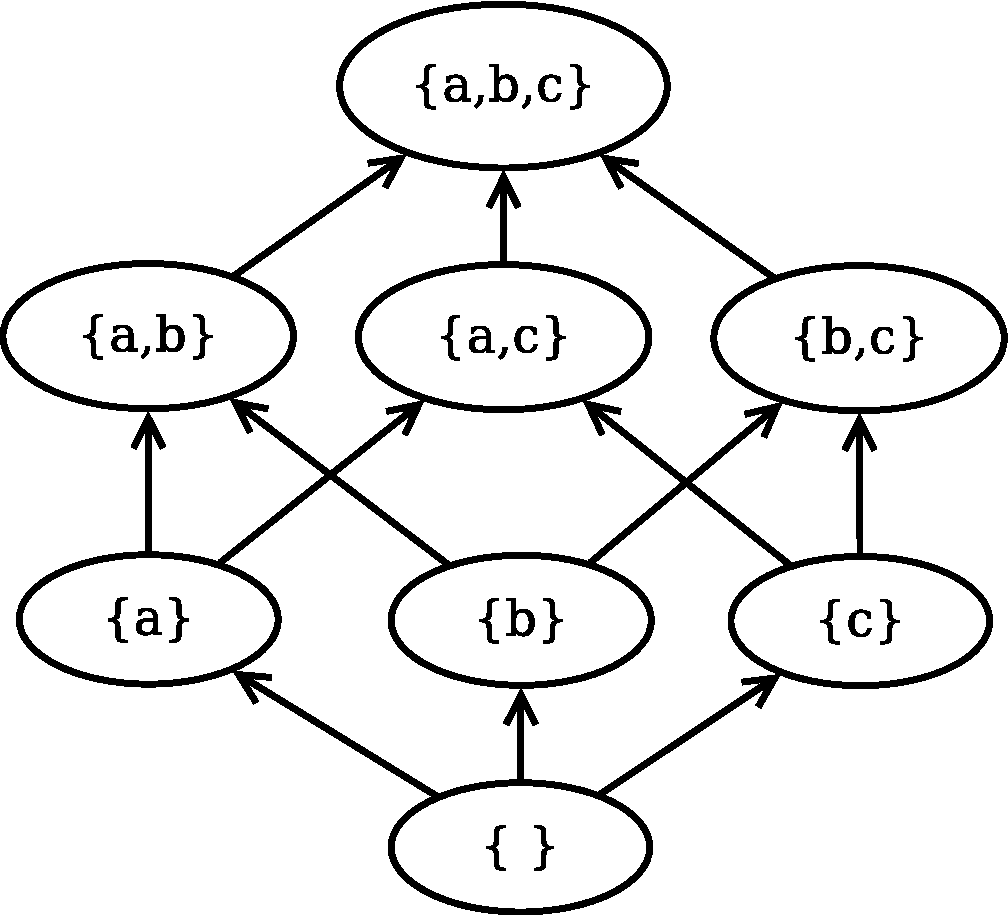
\includegraphics[width=.4\textwidth]{Figures/diagrama_hasse.pdf}
\caption{Conjunto das partes ilustrado por um diagrama de \emph{Hasse}}
\label{fig:diagrama_hasse}
\end{figure}

A inova��o do \textit{Apriori} sobre a abordagem ing�nua � a redu��o da
quantidade de conjuntos candidatos pelo descarte de certos conjuntos que
comprovadamente n�o s�o conjuntos frequentes. Desta forma o algoritmo
consegue detectar todos os conjuntos frequentes sem a necessidade de calcular o
suporte para todos os $2^n$ subconjuntos poss�veis.

A descoberta de conjuntos frequentes acontece por n�veis, como uma busca em
largura no diagrama de \emph{Hasse} come�ando pelos conjuntos unit�rios. Ao
inv�s de gerar os conjuntos candidatos a partir da base de dados, a cada n�vel
da busca � feita uma combina��o dos elementos para gerar os candidatos do n�vel
seguinte. Neste ponto a solu��o se beneficia do seguinte princ�pio: qualquer
subconjunto de um conjunto frequente tamb�m � um conjunto frequente. Portanto,
s� devem participar da nova combina��o os elementos que apresentarem um suporte
superior ao limite, pois um conjunto que n�o � frequente n�o ser� jamais
subconjunto de um conjunto frequente \cite{Agrawal:94}.

A figura \ref{fig:diagrama_apriori} ilustra a descoberta dos conjuntos
frequentes em contraposi��o com o conjunto das partes do conjunto $U =
\{a,b,c,d,e\}$. Neste exemplo, os subconjuntos $\{e\}$, $\{a,b\}$ e $\{b,d\}$
est�o destacados por apresentarem suporte inferior ao limite. Consequentemente,
todos os conjuntos dos quais estes s�o subconjuntos foram desconsiderados como
conjuntos candidatos (n�s com fundo cinza na figura). Portanto, apenas os n�s
com fundo branco teriam o suporte calculado.

\begin{figure}[ht]
\centering
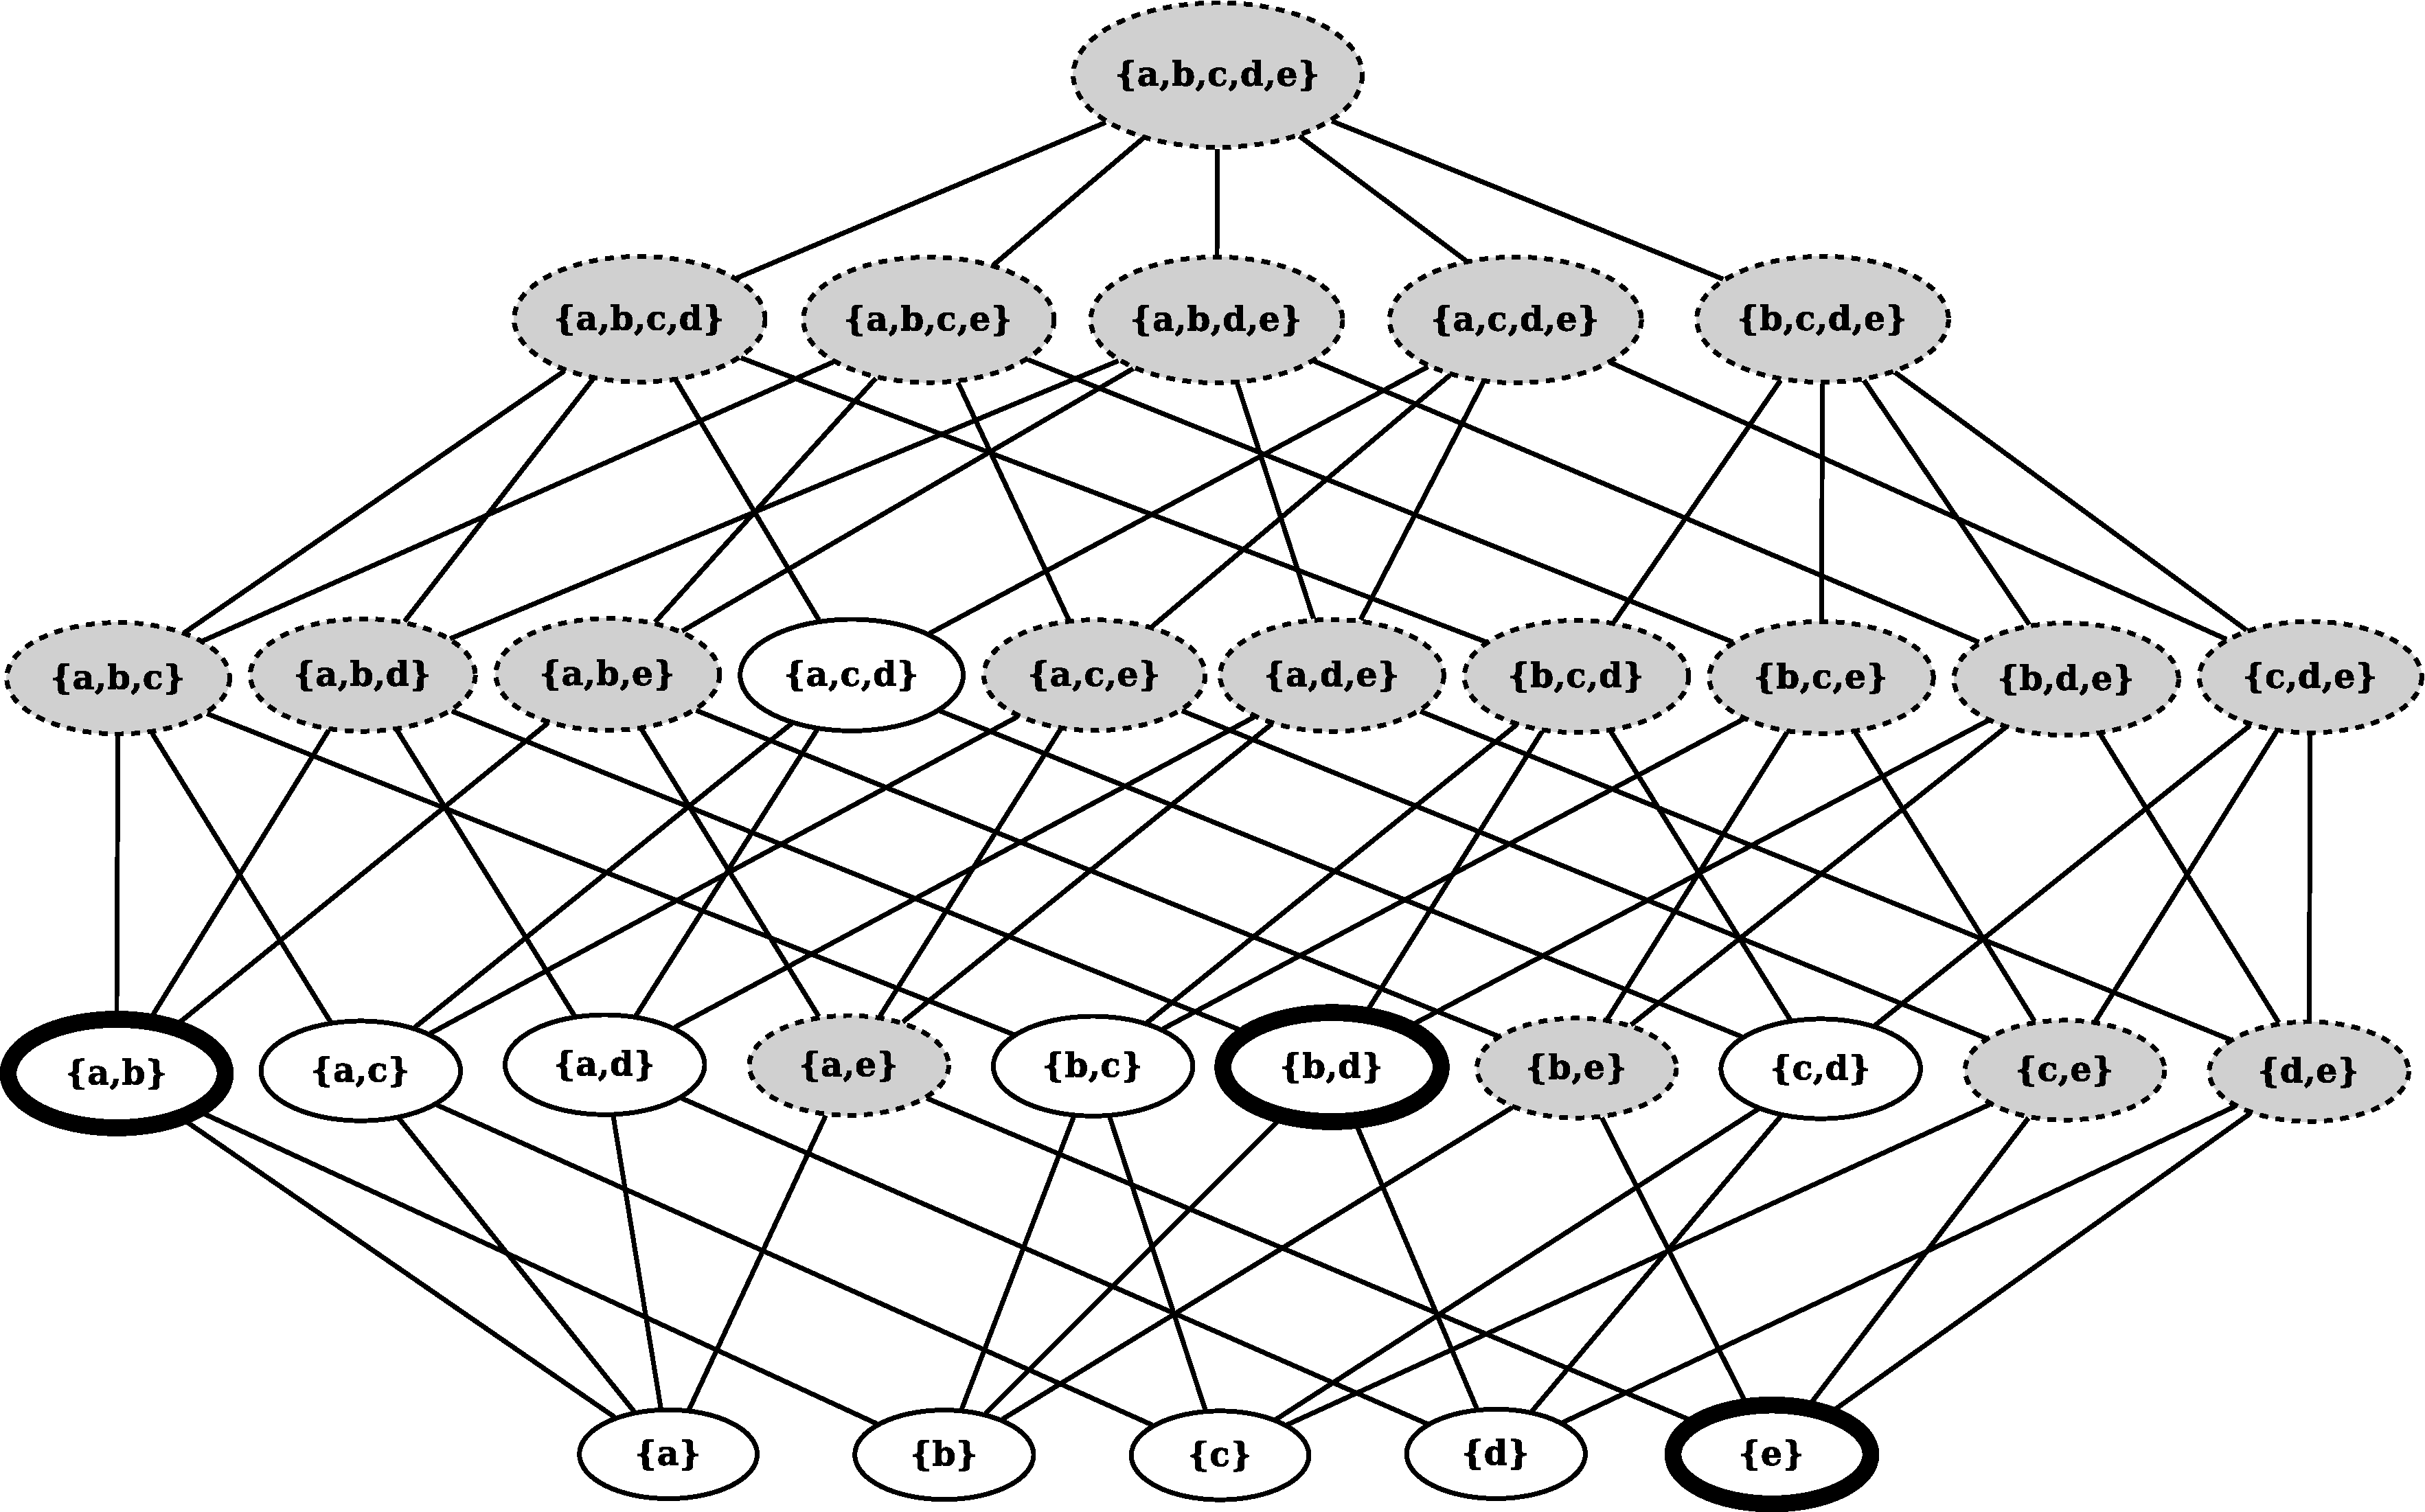
\includegraphics[width=\textwidth]{Figures/diagrama_apriori.pdf}
\caption{Gera��o de conjuntos candidatos pelo algoritmo Apriori}
\label{fig:diagrama_apriori}
\end{figure}

%http://www.slidefinder.net/d/data_mining_association_analysis_basic/14431678

A introdu��o do \textit{Apriori} representou um marco para o desenvolvimento de
solu��es para minera��o de dados, motivando o surgimento de in�meras variantes
baseadas no mesmo princ�pio. Entre elas, surgiram algumas propostas espec�ficas
para situa��es onde os dados t�m caracter�sticas adicionais conhecidas como,
por exemplo, base de dados particionada, dados que satisfazem � determinadas
restri��es ou que fazem parte de uma taxonomia conhecida \cite{Hegland:03}.

Apesar de apresentar um processo inovador para gera��o de regras de associa��o,
o \textit{Apriori} tamb�m apresenta fraquezas, sendo a principal delas a
necessidade de percorrer a base de dados m�ltiplas vezes para c�lculo de
suporte e confian�a dos conjuntos de itens. Algumas solu��es alternativas
fazem uso de estruturas de dados auxiliares para armazenar informa��es
extra�das da base de dados numa �nica passagem, evitando desta forma repetidos
acessos � mesma. �rvores de prefixos, �rvores lexicogr�ficas e matrizes
bin�rias s�o algumas dessas estruturas \cite{Kotsiantis:06}.

\section{Estrat�gias de recomenda��o} \label{sec:estrategias}

Neste trabalho considera-se uma classifica��o mista dos seguintes autores.
\cite{Burke:02} distingue as diferentes estrat�gias de recomenda��o a partir
da fonte de dados de onde � extra�do o conhecimento para produzir as
recomenda��es. \cite{Cazella:10} prop�e uma classifica��o um pouco mais
abrangente, considerando por exemplo a recomenda��o por reputa��o dos itens,
que por n�o oferecer grandes desafios computacionais � omitida por algumas
taxonomias.

\subsection{Reputa��o dos itens}

Popular entre servi�os de venda como livrarias, sites de leil�o e
lojas de modo geral, esta estrat�gia consiste no armazenamento de avalia��es
dos produtos escritas por usu�rios, bem como na apresenta��o das mesmas no
momento e local apropriado \cite{Cazella:10}. A implementa��o desta solu��o �
simples, visto que exige apenas a manuten��o dos dados originais, n�o sendo
necess�ria an�lise posterior alguma. No entanto, tem-se como premissa a
imparcialidade dos usu�rios em suas opini�es, que de fato n�o pode ser
verificada devido a seu car�ter subjetivo e estritamente pessoal. Atualmente
existem servi�os especializados em reputa��o de produtos que n�o realizam
venda associada, apenas disponibilizam as avalia��es. � o caso do
\textit{Internet Movie Database} \footnote{\url{http://www.imdb.com/}},
apresentado na figura \ref{fig:imdb}.

\begin{figure}[h!]
\centering
\fbox{
  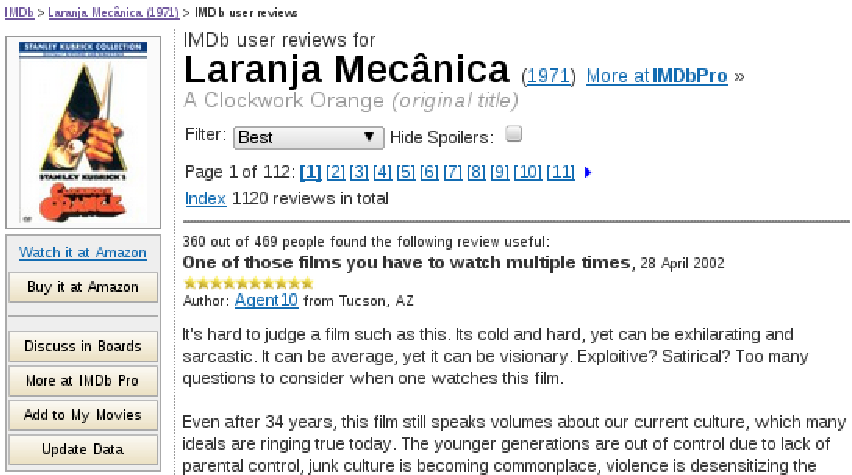
\includegraphics{Figures/imdb.pdf}
}
\caption{Avalia��o de usu�rio no IMDb}
\label{fig:imdb}
\end{figure}

\subsection{Recomenda��o baseada em conte�do}

Esta abordagem parte do princ�pio de que os usu�rios tendem a se interessar por
itens semelhantes aos que eles j� se interessaram no passado
\cite{Herlocker:00}. O ponto chave desta estrat�gia � a caracteriza��o dos
itens, por exemplo, atrav�s da identifica��o de atributos (autores e temas de
livros, por exemplo). A partir dos atributos dos itens, aplica-se t�cnicas de
recupera��o da informa��o (por exemplo, $\tfidf$ e \textit{BM25}) para
encontrar itens semelhantes ou de classifica��o (por exemplo, \textit{Bayes
ing�nuo} e \textit{K-NN}) para encontrar itens relevantes. Em uma livraria,
sugerir ao cliente outros livros do mesmo autor ou tema de livros previamente
selecionados � uma estrat�gia amplamente adotada.

\begin{figure}[h!]
\centering
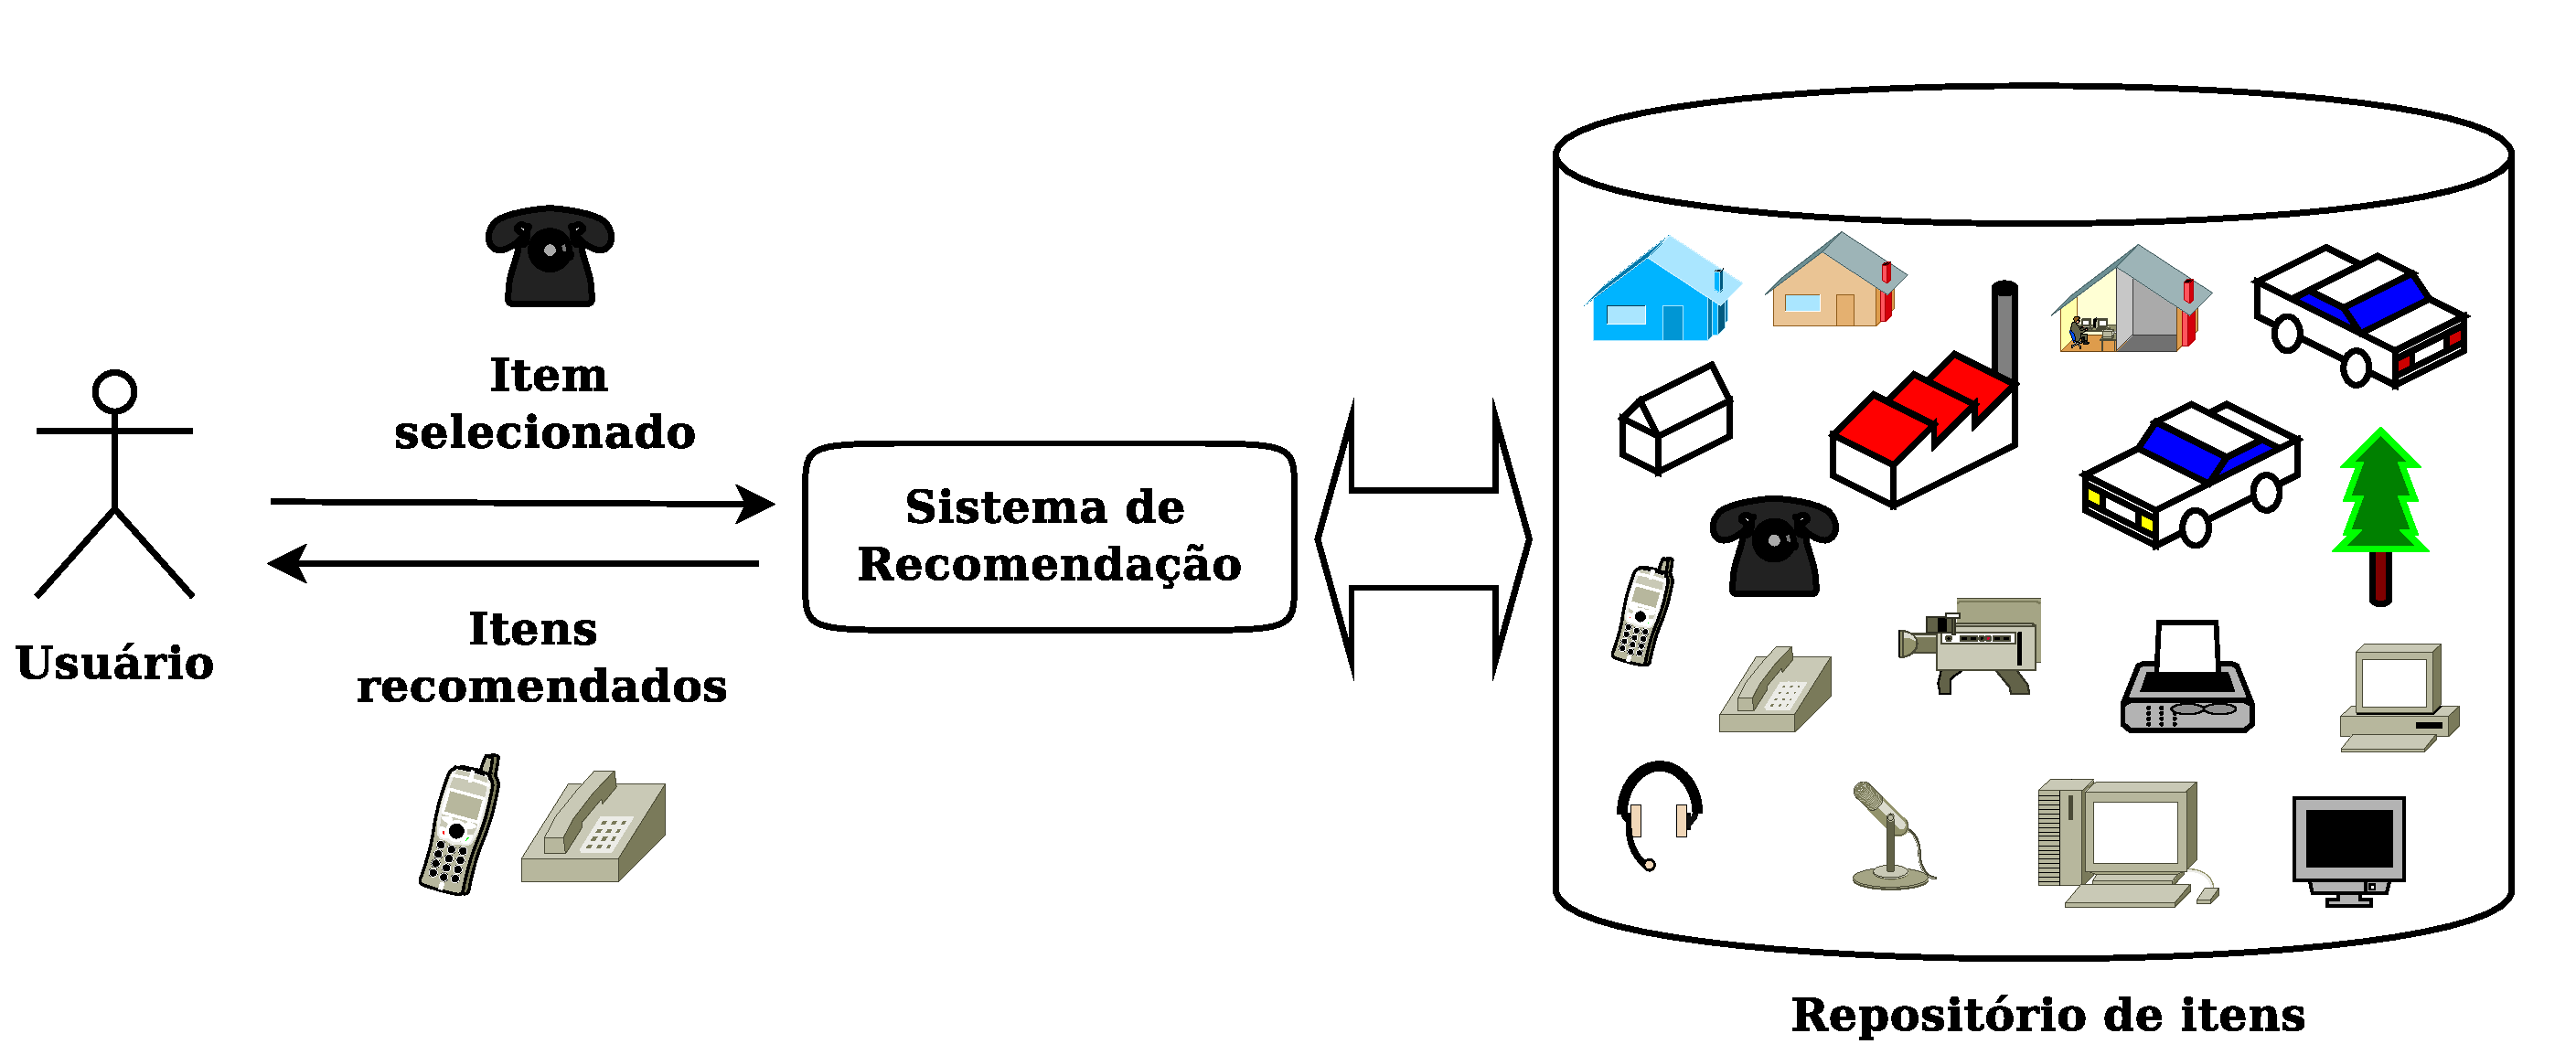
\includegraphics[width=\textwidth]{Figures/rec_conteudo.pdf}
\caption{Cen�rio de uma recomenda��o baseada em conte�do}
\label{fig:rec_conteudo}
\end{figure}

Pelo fato de se apoiar na classifica��o dos itens, os resultados da
recomenda��o s�o prejudicados nos casos em que os atributos n�o podem ser
identificados de forma automatizada. A superespecializa��o � outro problema
indicado por \cite{Adomavicius:05}, que diz respeito � abrang�ncia das
recomenda��es estar limitada a itens similares aos j� escolhidos pelos usu�rios.

\subsection{Recomenda��o colaborativa}

Esta estrat�gia n�o exige o reconhecimento sem�ntico do conte�do dos itens,
pois � fundamentado na troca de experi�ncias entre indiv�duos que possuem
interesses em comum. A figura \ref{fig:rec_colaborativa} ilustra o cen�rio da
recomenda��o colaborativa.

\begin{figure}[h!]
\centering
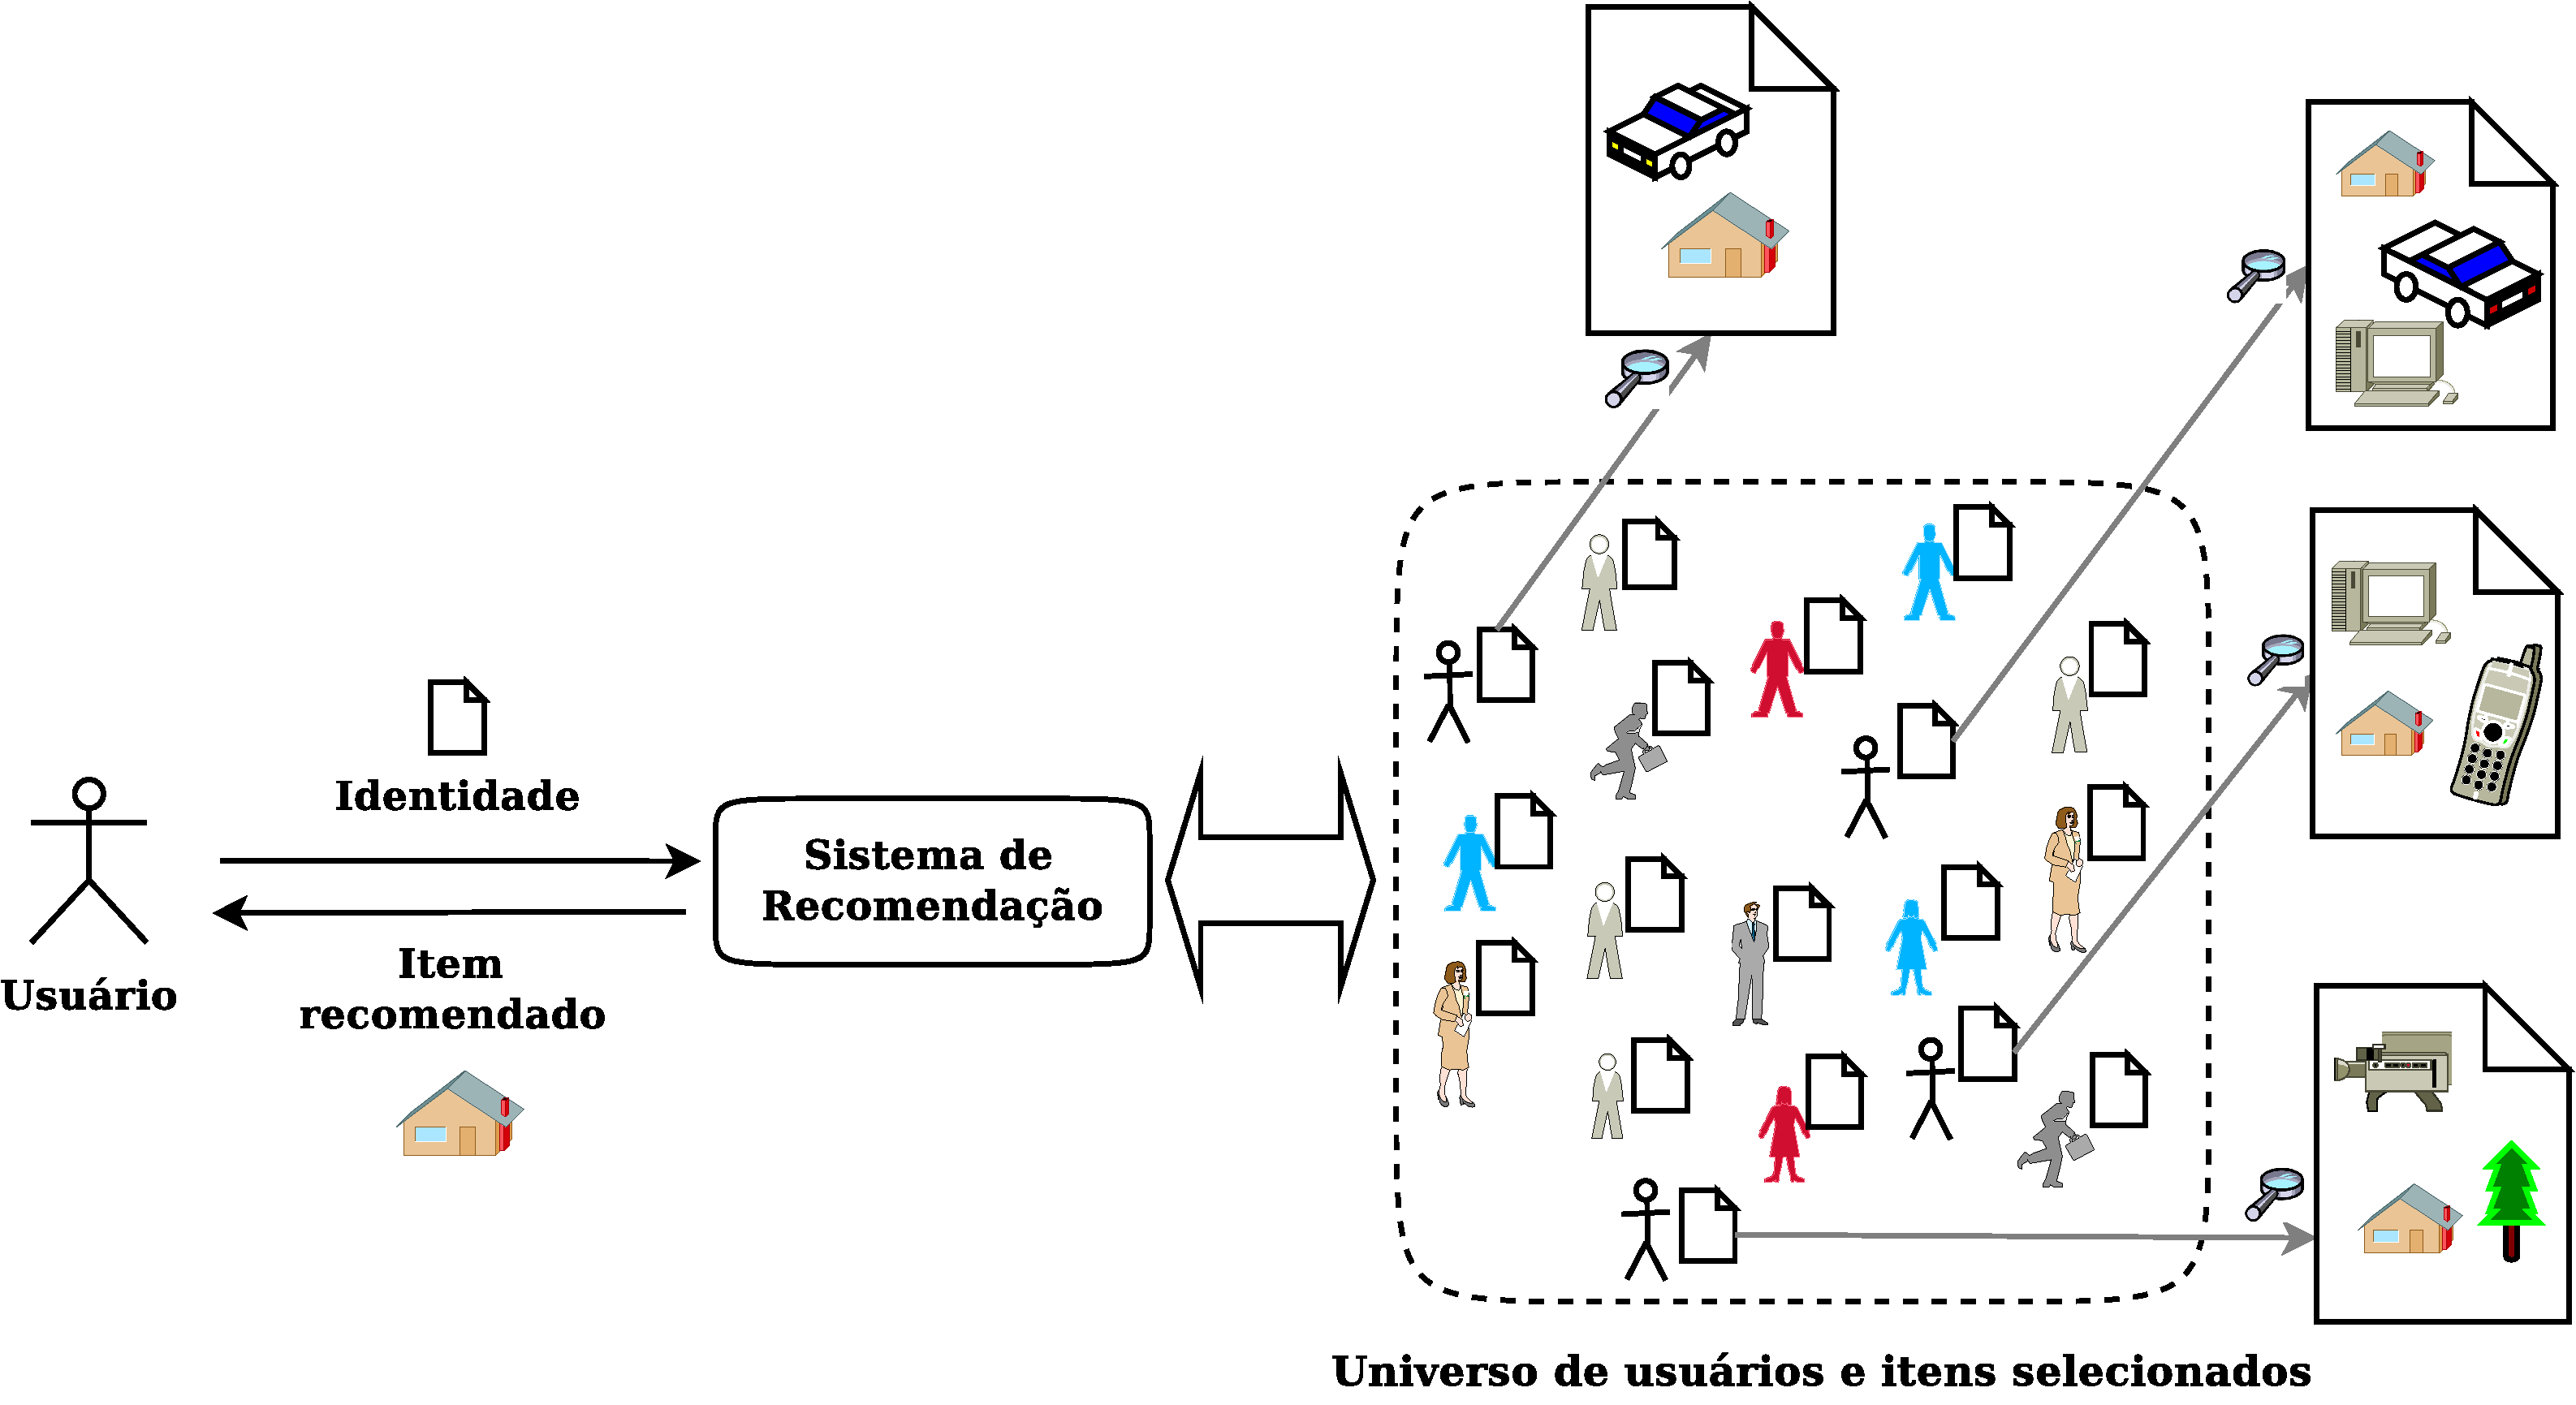
\includegraphics[width=\textwidth]{Figures/rec_colaborativa.pdf}
\caption{Cen�rio da recomenda��o colaborativa}
\label{fig:rec_colaborativa}
\end{figure}

A t�cnica \textit{K-NN} � comumente utilizada neste tipo de solu��o. Define-se
uma fun��o que representa a proximidade entre os usu�rios. Com base nesta
medida, a vizinhan�a de um determinado usu�rio � composta por outros $k$
usu�rios que estiverem mais pr�ximos a ele. Por�m, ao inv�s de uma classe ser
extra�da da vizinhan�a, como descrito na se��o \ref{sec:knn}, uma recomenda��o
para o usu�rio � produzida a partir da an�lise dos itens que os usu�rios
vizinhos consideram relevantes. Geralmente os itens que ocorrem com maior
frequ�ncia na vizinhan�a comp�em a recomenda��o.

O problema da superespecializa��o � superado, visto que a recomenda��o neste
caso n�o se baseia no hist�rico do pr�prio usu�rio, portanto pode apresentar
itens totalmente inesperados. Outra contribui��o � a possibilidade de forma��o
de comunidades de usu�rios pela identifica��o de interesses semelhantes
\cite{Cazella:10}.

\subsection{Baseada em conhecimento}

Esta estrat�gia tem como princ�pio a descoberta de conhecimento a partir da
an�lise de uma base de dados de transa��es, que registra a escolha dos usu�rios
ao longo do tempo. T�cnicas de classifica��o e minera��o de dados s�o
utilizadas para extrair correla��es e padr�es frequentes no comportamento dos
usu�rios. Tal abordagem � frequentemente utilizada em recomenda��es impl�citas,
por exemplo, na defini��o do posicionamento de produtos numa prateleira ou a
realiza��o de propagandas dirigidas \cite{Hegland:03}.

Agrupamento (\textit{clustering}, em ingl�s) � uma t�cnica de aprendizado de
m�quina n�o supervisionado. O algoritmo particiona a base de dados de forma a
criar automaticamente grupos que re�nam usu�rios com comportamentos
semelhantes. Uma das t�cnicas mais utilizadas � o $k\mhyphen means$, que
consiste basicamente em: (1) sele��o de $k$ usu�rios considerados sementes; (2)
associar cada usu�rio da base de dados com a semente mais pr�xima dele; (3)
calcular novos elementos centrais para cada grupo, entre os usu�rios que o
comp�em. O passo 3 � repetido at� que n�o seja mais necess�rio calcular novos
centr�ides. Desta forma, um sistema de recomenda��o poderia sugerir itens de
acordo com as caracter�sticas de cada grupo \cite{Cazella:10}.

Para descoberta de regras de associa��o, as t�cnicas mais utilizadas s�o
varia��es do algoritmos Apriori, apresentado na se��o \ref{sec:apriori}
\cite{Kotsiantis:06}. Dado um conjunto de associa��es, a recomenda��o para
determinado usu�rio � produzida de acordo com as regras satisfeitas pelo
conjunto de itens que ele j� tenha selecionado. Por exemplo, a regra ${A,B,C}
\Rightarrow {D}$ seria satisfeita por usu�rios que possuem os itens $A$, $B$ e
$C$, resultando na indica��o do item $D$: \textit{``Clientes que compraram os
itens A, B e C tamb�m compraram o item D''}. Um exemplo de recomenda��o por
associa��o � encontrado na loja virtual da empresa \textit{Amazon}\footnote{\url{http://www.amazon.com/}} (figura \ref{fig:amazon}).

\begin{figure}[h!]
\centering
\fbox{
  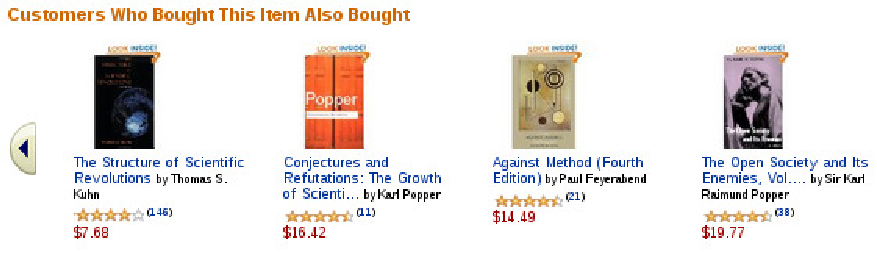
\includegraphics{Figures/amazon.pdf}
}
\caption{Recomenda��o por associa��o na Amazon}
\label{fig:amazon}
\end{figure}

\subsection{Baseada em dados demogr�ficos}

A estrat�gia demogr�fica fundamenta-se na composi��o de perfis de usu�rios e
identifica��o de nichos demogr�ficos para produ��o de recomenda��es. Os dados
pessoais geralmente s�o coletados de forma expl�cita, atrav�s de um cadastro
do usu�rio, e podem englobar informa��es como idade, sexo, profiss�o e �reas de
interesse. Dados demogr�ficos, no entanto, geralmente s�o utilizados em
combina��o com outras fontes de dados e t�cnicas diversas, como parte de uma
estrat�gia de recomenda��o h�brida.

\subsection{Estrat�gia h�brida} \label{sec:estrategias_hibrida}

Sistemas de recomenda��o h�bridos combinam duas ou mais estrat�gias, com o
intuito de obter melhor performance do que a que as estrat�gias oferecem
individualmente. A tabela \ref{tab:metodos_hibridizacao} apresenta as
principais t�cnicas de hibridiza��o, segundo \cite{Burke:02}.

\begin{table}[h!]
\caption{M�todos de hibridiza��o}
\label{tab:metodos_hibridizacao}
\small
\begin{tabularx}{\textwidth}{| l | X |}
\hline
\normalsize{\textbf{\textit{M�todo}}} &
\normalsize{\textbf{\textit{Descri��o}}} \\
\hline
Pondera��o & Pontua��es de relev�ncia oriundas de diversas t�cnicas de
             recomenda��o s�o combinadas para compor uma �nica recomenda��o. \\
\hline
Revezamento & O sistema reveza entre t�cnicas de recomenda��o diversas, de
              acordo com a situa��o do momento. \\
\hline
Combina��o & Recomenda��es oriundas de diversos recomendadores diferentes s�o
             apresentados de uma s� vez. \\
\hline
Combina��o de atributo & Um algoritmo de recomenda��o �nico coleta atributos
                         de diferentes bases de dados para recomenda��o. \\
\hline
Cascata & Um recomendador refina a recomenda��o produzida por outro. \\
\hline
Acr�scimo de atributo & O resultado de uma t�cnica � usado como atributo de
                        entrada para outra. \\
\hline
Meta-n�vel & O modelo que um recomendador ``aprendeu'' � usado como entrada
             para o outro. \\
\hline
\end{tabularx}
\end{table}

\section{Avalia��o de sistemas de recomenda��o} \label{sec:avaliacao}

A avalia��o de sistemas de recomenda��o n�o � uma tarefa trivial,
principalmente porque n�o h� consenso sobre quais atributos devem ser
observados e quais m�tricas devem ser adotadas para cada atributo
\cite{Herlocker:04}. Ademais, diferentes estrat�gias podem funcionar melhor
ou pior de acordo com o dom�nio da aplica��o e as propriedades dos dados.
Por exemplo, algoritmos projetados especificamente para conjuntos de dados com
um n�mero muito maior de usu�rios do que de itens podem se mostrar
inapropriados em dom�nios onde h� muito mais itens do que usu�rios.
Recomenda-se ent�o que o processo de avalia��o tenha in�cio com a compreens�o
das a��es para as quais o sistema foi projetado (ver se��o \ref{sec:acoes}),
como guia para as decis�es metodol�gicas ao longo dos experimentos.

\subsection{Sele��o dos dados}

A escolha do conjunto de dados adequado � fator chave para uma investiga��o
consistente. Neste aspecto, as avalia��es de recomendadores podem ser
caracterizadas como (a) an�lises \textit{offline}, que utilizam bases de dados
previamente coletadas e (b) experimentos ``ao vivo'', realizados diretamente
com usu�rios, seja num ambiente controlado (laborat�rio) ou em campo
\cite{Herlocker:04}.

An�lises \textit{offline} geralmente s�o objetivas, com foco na acur�cia das
predi��es e performance das solu��es \cite{Vozalis:03}. Inicialmente os dados
s�o particionados em por��es de treinamento e de testes. Utiliza-se como base
os dados de treinamento para prever recomenda��es para itens da por��o de
testes. Em seguida � feita a an�lise comparativa entre os resultados obtidos
e os esperados. Algumas m�tricas comumente utilizadas na fase de an�lise ser�o
apresentadas na se��o \ref{sec:metricas}. No entanto, tais an�lises s�o
prejudicadas em conjuntos de dados esparsos. N�o se pode, por exemplo, avaliar
a exatid�o da recomenda��o de um item para um usu�rio se n�o existe uma
avalia��o pr�via do usu�rio para tal item.

Por outro lado, nos experimentos ``ao vivo'' os recomendadores s�o
disponibilizados para uma comunidade de usu�rios, cujas avalia��es s�o
coletadas na medida em que s�o produzidas. Neste caso, al�m de an�lises
objetivas como a acur�cia e performance das solu��es, pode-se avaliar fatores
comportamentais como a performance, participa��o e satisfa��o dos usu�rios.
A esparsidade dos dados tem efeito menor neste tipo de experimento, visto
que o usu�rio est� dispon�vel para avaliar se os itens recomendados s�o ou
n�o relevantes.

Quando n�o existem dados previamente dispon�veis ou quando n�o s�o adequados
para o dom�nio ou a a��o principal do sistema a ser avaliado, pode-se ainda
optar pelo uso de dados sint�ticos. O uso de dados artificiais � aceit�vel
em fases preliminares de testes, por�m, tecer conclus�es comparativas �
arriscado visto que os dados produzidos podem se ajustar melhor para uma
estrat�gia do que para outras \cite{Herlocker:04}.

\section{M�tricas} \label{sec:metricas}

A tabela \ref{tab:metricas} apresenta m�tricas utilizadas para avalia��o de
sistemas de recomenda��o.

As m�tricas de acur�cia medem o quanto as estimativas de relev�ncia previstas
pelo sistema se aproximam da real. Acur�cia de classifica��o est� relacionada
com a frequ�ncia com a qual o sistema faz classifica��es corretas acerca da
relev�ncia dos itens, enquanto que a acur�cia de predi��o pondera as
diferen�as entre as pontua��es de relev�ncia prevista e a real.

Al�m de medidas de acur�cia, s�o apresentados outras m�tricas para mensurar
qualidades que proporcionam maior grau de satisfa��o do usu�rio ao utilizar um
sistema de recomenda��o.

\begin{sidewaystable}
\caption{M�tricas para avalia��o de sistemas recomendadores}
\label{tab:metricas}
\newcommand\T{\rule{0pt}{3.0ex}}
\newcommand\B{\rule[-1.8ex]{0pt}{0pt}}
\begin{tabularx}{\textwidth}{| c | X | c | c |}
\hline
\textbf{\textit{M�trica}} & \textbf{\textit{Descri��o}}
  & \textbf{\textit{F�rmula}}  & \textbf{\textit{Categoria}} \\
\hline
\T Precis�o & Propor��o de itens relevantes entre os selecionados
  & \multirow{2}{*}{$P = \frac{N_{\text{relevantes\ selecionados}}}
                              {N_{\text{selecionados}}}$}
  & \multirow{7}{*}{Acur�cia de classifica��o} \\
  & como tal \B & & \\
\cline{1-3}
\T Recupera��o & Propor��o de itens selecionados entre todos os
  & \multirow{2}{*}{$R = \frac{N_{\text{relevantes\ selecionados}}}
                              {N_{\text{relevantes}}}$} & \\
  & relevantes \B & & \\
\cline{1-3}
\T Medida $F_1$ & Combina��o de $P$ e $R$ numa mesma medida
  & \T\B $F_1 = \frac{2PR}{P+R}$ & \\
\cline{1-3}
\T Curva \textit{ROC} & Mede o poder de distin��o entre itens relevantes e
  & \scriptsize{An�lise gr�fica}& \\
  & irrelevantes \B & & \\
\hline
\T Erro absoluto m�dio & Desvio absoluto m�dio  entre pontua��es previstas e
 & \multirow{2}{*}{$|\overline E|=\frac{\sum_{i=1}^N |p_i-r_i|}{N} $}
 & \multirow{4}{*}{Acur�cia de predi��o} \\
 \textit{(MAE)} & reais \B & & \\
\cline{1-3}
\T Erro quadr�tico m�dio & Desvio quadr�tico m�dio entre pontua��es previstas e
  & \multirow{2}{*}{$|\overline E|=\frac{\sum_{i=1}^N |p_i-r_i|^2}{N}$ }& \\
  & reais \B & & \\
\hline
\T Cobertura & Propor��o de itens pass�veis de serem recomendados
  & \multirow{2}{*}{$R = \frac{N_{\text{pass�veis de recomenda��o}}}{N}$}
  & \multirow{5}{*}{Al�m de acur�cia} \\
  & entre todos os dispon�veis \B & & \\
\cline{1-3}
\T Curva de aprendizado & Taxa de aprendizado dos algoritmos na an�lise dos
  & \multirow{2}{*}{$A = \frac{\Delta_\text{acur�cia}}{\Delta_T}$} & \\
  & dados de exemplo \B & & \\
\cline{1-3}
\T Novidade e surpresa & Qualidade do sistema de produzir recomenda��es
  & \scriptsize{Avaliada pelo usu�rio} & \\
  & n�o �bvias \B & & \\
\hline
\end{tabularx}
\end{sidewaystable}

\newpage

\chapter{Trabalhos correlatos} \label{chapter:trab-correlatos}

No presente cap�tulo ser�o apresentadas iniciativas de desenvolvimento por
parte da comunidade FOSS e trabalhos acad�micos que se relacionam com a
proposta deste trabalho. Algumas dessas iniciativas foram utilizadas como base
de desenvolvimento, principalmente as relativas ao projeto Debian, enquanto
outras serviram como fontes de refer�ncias e inspira��o.
%FIXME [questionamento aos desenvolvedores sobre razao da descontinuidade]

\section{Iniciativas FOSS}
% FIXME [Pesquisar sobre contexto em outras distros]

\subsection{Dados sobre pacotes Debian}

O projeto Debian tem se destacado no universo das distribui��es por suas
iniciativas pioneiras no campo de gerenciamento de aplica��es \cite{Zini:11}.
Diante da complexa e crescente estrutura do projeto, observa-se um esfor�o por
parte dos desenvolvedores, principalmente da equipe respons�vel pelo controle
de qualidade\footnote{\url{http://qa.debian.org}}, de reunir, organizar e
disponibilizar as informa��es ou meta-dados concernentes a esta estrutura
\cite{Nussbaum:10}.

A seguir ser�o detalhadas algumas destas iniciativas, que curiosamente foram
desenvolvidas inicialmente num contexto extra-oficial e, ao passo que se
mostraram �teis e eficientes, foram absorvidas pela comunidade de usu�rios e
desenvolvedores.

%screenshots.debian.net: web service providing app screenshot

\subsubsection{Debtags}

\textit{Debtags} � um esquema de classifica��o idealizado pelo desenvolvedor
Debian Enrico Zini como uma maneira de categorizar pacotes alternativa �s
se��es \cite{Zini:05}. A principal motiva��o desta iniciativa foi a
impossibilidade de relacionar pacotes a m�ltiplas se��es. Um navegador web, por
exemplo, n�o poderia ser categorizado como \textit{network} e \textit{web}
simultaneamente. O uso de \textit{tags} (em portugu�s, r�tulos) possibilitaria
a cria��o de uma cole��o estruturada de metadados que poderia ser utilizada
para implementar m�todos mais avan�ados do que os existentes para apresenta��o,
busca e manuten��o do reposit�rio de pacotes Debian.

O proposta foi apresentada na Debconf5 e foi paulatinamente sendo adotada por
desenvolvedores em suas atividades, sendo atualmente utilizada como base de
in�meras ferramentas no Debian, tendo atingido a marca de $45\%$ de pacotes
categorizados\footnote{Consulta realizada em junho de 2011}.
%[FIXME] checar sobre os 45% na lista

Utilizando \textit{Debtags}, os pacotes podem ser caracterizados por m�ltiplos
atributos, que s�o (propositalmente) definidos num momento posterior �
concep��o do pacote. Dado que a base de tags � mantida de forma independente ao
reposit�rio, as modifica��es ao longo do tempo n�o trazem impacto algum ao
desenvolvimento de pacotes. A atribui��o de tags a pacotes � realizada por
colaboradores atrav�s do website do projeto\footnote{\url{http://debtags.alioth.debian.org/todo.html}} e revisada manualmente antes de ser incorporada � base
de dados.

A base de dados � armazenada num arquivo texto no formato da figura
\ref{fig:debtags}. O conjunto de tags dispon�vel faz parte de um vocabul�rio
controlado\footnote{\url{http://debtags.alioth.debian.org/vocabulary/}}, que
tamb�m recebe contribui��es de colaboradores. O esquema � estruturado para
permitir a classifica��o por diferentes pontos de vista, que caracterizam as
facetas.

\begin{figure}
\label{fig:debtags}
\begin{verbatim}
acx100-source: admin::kernel, implemented-in::c, role::source,
use::driver

adduser: admin::user-management, implemented-in::perl,
interface::commandline, role::program, scope::utility

apache2: implemented-in::c, interface::daemon, network::server,
network::service, protocol::http, protocol::ipv6, role::metapackage,
role::program, suite::apache, web::server, works-with-format::html,
works-with::text

apbs: field::chemistry, implemented-in::c, interface::commandline,
role::program, scope::utility

apcalc: field::mathematics, interface::shell, interface::text-mode,
role::program, scope::utility
\end{verbatim}
\caption{Excerto da base do Debtags}
\end{figure}

Ao indicar novas tags para um pacote, o usu�rio � surpreendido com sugest�es de
outras tags que geralmente s�o aplicadas em conjunto com as j� selecionadas.
Esta � uma aplica��o de recomenda��o com base em regras de associa��o
descobertas a partir de an�lise da base de dados de tags. O algoritmo utilizado
para produ��o das regras � o Apriori, descrito na se��o \ref{sec:apriori}.

O \textit{Debtags} � uma poderosa ferramenta para a constru��o de estrat�gias
de recomenda��o de pacotes baseadas em conte�do. � fato que o conte�do acerca
de pacotes pode ser expresso em termos de atributos extra�dos dos pr�prios
pacotes, por�m, a caracteriza��o por meio de tags j� fornece uma caracteriza��o
poss�vel de ser utilizada e a custo baixo.

\subsubsection{Apt-Xapian-Index}

\subsubsection{Popcon} \label{sec:popcon}

O \textit{Popcon (Popularity Contest)} � o concurso de popularidade entre
pacotes Debian, criado pelo desenvolvedor Avery Pennarun em 1998 com o
prop�sito inicial de auxiliar a escolha dos pacotes que fazem parte do primeiro
CD de instala��o\footnote{\url{http://lists.debian.org/debian-devel-announce/2004/03/msg00009.html}} (os mais populares s�o selecionados). Atualmente o
reposit�rio de pacotes Debian pode ser obtido em 52 imagens de CDs ou 8 de DVD.
Dado que comumente obtem-se apenas a primeira imagem por \textit{download}, a
A prioriza��o de pacotes populares na primeira imagem tende a contribuir para a
satisfa��o dos usu�rios, dado que geralmente apenas este � obtida por
\textit{download} e os demais pacotes s�o obtido diretamente do reposit�rio
por meio de uma conex�o de rede.

Na instala��o de um sistema Debian o usu�rio � convidado a participar do
concurso. Se aceitar, o software cliente do \textit{popcon} � instalado e envia
periodicamente a lista de pacotes daquele sistema para um servidor central,
indicando tamb�m quais deles foram utilizados recentemente. A figura
\ref{fig:popcon} apresenta um exemplo de submiss�o do popcon. A primeira linha
cont�m um hash que identifica um sistema unicamente no concurso (submiss�es
consecutivas de um mesmo usu�rios s�o sobrescritas). Cada linha seguinte
representa um pacote instalado no sistema, no formato
\verb!<atime> <ctime> <package-name> <mru-program> <tag>!, detalhado na tabela
\ref{tab:popcon}. Os campos relativos a tempo s�o indicados no formato
\textit{Unix time\_t}\footnote{Quantidade de segundos desde meia-noite de
primeiro de janeiro de 1970 no hor�rio GMT.}.

\begin{figure}[h!]
\begin{verbatim}


POPULARITY-CONTEST-0 TIME:914183330 ID:b92a5fc1809d8a95a12eb3a3c84166dd
914183333 909868335 grep /bin/fgrep
914183333 909868280 findutils /usr/bin/find
914183330 909885698 dpkg-awk /usr/bin/dpkg-awk
914183330 909868577 gawk /usr/bin/gawk
[...]
[...]
[...]
END-POPULARITY-CONTEST-0 TIME:914183335
\end{verbatim}
\caption{Exemplo de submiss�o do popcon}
\label{fig:popcon}
\end{figure}

\begin{table}[h!]
  \centering
  \newcommand\T{\rule{0pt}{2.8ex}}
  \newcommand\B{\rule[-1.8ex]{0pt}{0pt}}
  \begin{tabularx}{15cm}{| l | X |}
    \hline
    \textbf{Campo} & \textbf{Descri��o} \\
    \hline
    <package-name> & nome do pacote Debian que cont�m <mru-program>\\
    \hline
    <mru-program> & Programa, biblioteca ou cabe�alho contido no pacote
                    que foi utilizado mais recentemente.\\
    \hline
    <atime> & Tempo de acesso do <mru-program> no disco, atualizado pelo
                     kernel cada vez que o arquivo � aberto.\\
    \hline
    <ctime> & Tempo de cria��o do <mru-program> no disco, definido no
                     momento de instala��o do pacote.\\
    \hline
    <tag> & RECENT-CTIME: indica que <atime> � muito pr�ximo de <ctime>,
            geralmente quando o pacote foi recentemente instalado ou
            atualizado; OLD: <atime> � anterior a um m�s atr�s, portanto o
            pacote n�o foi usado no �ltimo m�s; NOFILES: o pacote n�o cont�m
            programas, portanto <atime>, <ctime> e <mru-program> s�o
            inv�lidos.\\
    \hline
  \end{tabularx}
  \caption{Descri��o do formato de uma submiss�o popcon}
  \label{tab:popcon}
\end{table}

As submiss�es recebidas s�o processadas diariamente e as estat�sticas geradas
s�o disponibilizadas no website do projeto\footnote{\url{http://popcon.debian.org}}.
Os dados ``crus'' (listas de pacotes antes de serem processadas) j� foram
utilizados anteriormente para fins de minera��o de dados, como descrito nas
se��es \ref{sec:anapop} e \ref{sec:mining_popcon}, por�m ambos os trabalhos
foram descontinuados.

A informa��o sobre o uso dos pacotes tamb�m tem sido utilizada como guia para o
time de qualidade acerca de quais pacotes merecem aten��o especial. Os times de
trandu��o igualmente t�m considerado estes dados para ordenar a lista de
prioridades de acordo com a popularidade. Por outro lado, pacotes
``problem�ticos'' (p. ex. pacotes com muitos \textit{bugs RC}, �rf�os ou com
mantenedor em MIA) que apresentam baixa popularidade tendem a perder a simpatia
dos desenvolvedores, sendo esta um dos par�metros para a decis�o de remover um
pacote do reposit�rio (\textit{low-popcon}).

Essa abordagem, no entanto, tem sido duramente criticada. Segundo Joey
Hess\footnote{\url{http://kitenet.net/~joey/blog/entry/the_popcon_problem/}},
uma vantagem do Debian � justamente que n�o apenas programas populares s�o
empacotados, mas os incomuns e espec�ficos de um nicho de usu�rio tamb�m
costumam estar dispon�veis em pacotes. E de fato o \textit{popcon} n�o mede o
benef�cio de pacotes poucos usados estarem dispon�veis no reposit�rio, prontos
para serem usados. Enquanto que ao remover pacotes que aparentemente n�o s�o
populares, corre-se o risco de transformar o Debian numa distribui��o
homog�nea, submetida � ``tirania da maioria''.

Existem ainda quest�es relativas a (1) representatividade desses dados, visto
que alguns perfis de usu�rios dificilmente participam do concurso (p. ex.
sistemas embarcados); e (2) acur�cia de informa��es temporais, dado que
\verb!<atime>! e \verb!<ctime>! podem ser inconsistentes caso o sistema de
arquivos tenha sido montado com a op��o \verb!noatime!.

Todas essas ressalvas devem ser consideradas quando pretende-se utilizar os
dados do \textit{popcon}. No entanto, desde que as informa��es sejam manejadas
de forma consciente e respons�vel, acredita-se que valiosas correla��es possam
ser reveladas ap�s uma s�rie de an�lises.

\subsubsection{UDD}

Acr�nimo para \textit{Ultimate Debian Database}, o
UDD\footnote{\url{http://udd.debian.org}} � uma iniciativa recente do time de
qualidade criada com o intuito de reunir informa��es de diversos aspectos do
Debian numa base de dados �nica \cite{Nussbaum:10}.

O fluxo de dados do UDD � apresentado na figura \ref{fig:udd}. Existe um
coletor para cada tipo de fonte de dados (p. ex. o sistema de acompanhamento de
bugs\footnote{\url{http://bugs.debian.org}} que implementa uma interface comum e
esconde a complexidade e especificidade de acessar cada fonte de dados. Existe
um processo central no UDD que invoca os coletores periodicamente, provocando a
inser��o dos dados na base �nica.

\begin{figure}[h!]
\centering
  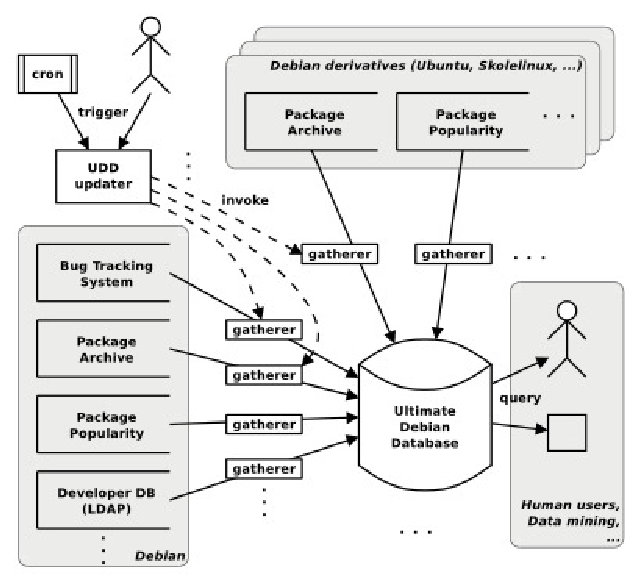
\includegraphics{Figures/udd.pdf}
\caption{Fluxo de dados no UDD \cite{Nussbaum:10}}
\label{fig:udd}
\end{figure}

A pricipal motiva��o para o desenvolvimento do UDD foi auxiliar o time de QA em
suas atividades, al�m de facilitar a colabora��o com distribui��es derivadas do
Debian. Apesar de ser poss�vel, dificilmente usu�rios consultariam esta base
para tomar decis�es acerca de que pacotes utilizar, visto que os dados
armazenados no UDD geralmente s�o acess�veis por outros meios. No entanto, para
fins de minera��o de dados ou para o desenvolvimento de um recomendador
autom�tico, a possibilidade de acesso a dados de tamanha heterogeneidade numa
fonte de dados �nica � uma grande vantagem.

%\subsection{DDE}
%
%Acr�nimo para \textit{Debian Data Export},
%DDE\footnote{\url{http://wiki.debian.org/DDE}}


\subsection{Dados sobre pacotes \textit{rpm}}

Apesar de n�o estarem diretamente relacionadas com o desenvolvimento deste
trabalho, a seguir s�o descritos alguns esfor�os recentes para coleta de dados
sobre pacotes \textit{rpm}.

\subsubsection{Sophie}

Ferramenta web\footnote{\url{http://sophie.zarb.org/}} que permite a busca e
an�lise do conte�do de pacotes rpms de m�ltiplas distribui��es. Prov� tamb�m
uma interface XML-RPC que possibilita a cria��o de outras ferramentas
utilizando Sophie como base.

\subsubsection{mageia-app-db}

Base de dados de aplicativos idealizada pelos desenvolvedores da distribui��o
Mageia\footnote{\url{http://mageia-app-db.tuxette.fr/projects/mageia-app-db/wiki}},
que atualmente tamb�m re�ne esfor�os de colaboradores do openSUSE, Mandriva e
Fedora. Ainda em fase de desenvolvimento, a ferramenta tem como principal
objetivo facilitar a intera��o entre usu�rios, testadores e empacotadores de
software. Al�m de acessar a cole��o de aplicativos dispon�veis na distribui��o,
o usu�rio ser� capaz de requisitar funcionalidades ou corre��es aos
respons�veis pelos pacotes, al�m de acompanhar seus pedidos e receber
notifica��es autom�ticas. Produ��o de recomenda��es de pacotes tamb�m est�o
previstas como funcionalidades do sistema.

%\subsection{openSUSE Software Portal}
%
%Ferramenta web dedicada a aplicativos do openSUSE em desenvolvimento desde o
%ano de 2007. Legado???

\subsection{Servidor para avalia��o de aplicativos}

Em ingl�s, \textit{Ratings and Reviews
Server}\footnote{\url{http://launchpad.net/rnr-server}}, � um servi�o em
desenvolvimento baseado em \textit{django}\footnote{\url{https://www.djangoproject.com/}} para armazenar avalia��es de usu�rios sobre
aplicativos, com pontua��o e coment�rios. Quando estiver em produ��o ser� uma
poderosa base de dados para a produ��o de recomenda��es sobre aplicativos,
alternativa � base do popcon, que n�o foi projetada para fins de recomenda��o e
se restringe a dados bin�rios (um usu�rio possue um pacote instalado ou n�o).

%not following the open-collaboration-spec yet, but there is interesst about
%this from the devs

\subsection{Open Collaboration Service}

Especifica��o aberta projetada para dar suporte a colabora��o entre servi�os
web, permitindo o armazendamento de avalia��es de usu�rios e outras informa��es
do dom�nio de aplica��o.

\subsection{AppStream}

Grande parte das distribui��es GNU/Linux t�m investido no desenvolvimento de
interfaces para facilitar o gerenciamento de aplicativos e a forma como se obt�m
informa��es sobre os mesmos. Entre os dias 18 e 21 de janeiro 2011 aconteceu a
primeira reuni�o sobre a tem�tica com a presen�a de desenvolvedores de
distribui��es variadas (\textit{Cross-distribution Meeting on Application
Installer}). O encontro teve como principais objetivos a defini��o de padr�es
entre os diferentes projetos no que diz respeito a: procedimentos de instala��o
de aplica��es; metadados associados aos pacotes; o modo como tais informa��es
devem ser geradas e armazenadas; protocolo para manuten��o de metadados
din�micos; e a defini��o de quais metadados devem ser compartilhados entre as
distribui��es, em detrimento de outros considerados espec�ficos de cada projeto
\cite{Freedesktop:11}.

% FIXME [Desenvolver texto sobre esfor�os inter-distribui��es]
% http://distributions.freedesktop.org/wiki/Meetings/AppInstaller2011
%app-install: UI focused on applications + code to generate metadata

\subsection{Anapop/PopSuggest} \label{sec:anapop}

O Anapop ou Popsuggest foi desenvolvido em 2007 por Enrico Zini\textit{PopSuggest}\footnote{\url{http://www.enricozini.org/2007/debtags/popcon-play/}}
como uma ilustra��o das possibilidades de uso dos dados coletados pelo popcon.
A ferramenta utilizava t�cnicas de recupera��o da informa��o sobre a base de
submiss�es do popcon para inferir quais pacotes diferenciavam determinado
usu�rio dos demais, al�m de sugerir pacotes que usu�rios similares �quele
tinham instalados.
% Fonte: http://wiki.yobi.be/wiki/Debian_Tricks

\section{Trabalhos acad�micos}

Nos �ltimos anos foram publicados, no Brasil e no exterior, in�meros trabalhos
nas �reas de minera��o de dados e recupera��o da informa��o aplicadas aos mais
diversos dom�nios de aplica��o. Nesta se��o nos restringimos a comentar alguns
deles que foram utilizados como refer�ncia, por tratarem especificamente do
problema de recomenda��o, no dom�nio de aplicativos ou n�o.

\subsection{\textnormal{\textit{``Uma aplica��o em sistemas de recomenda��o:
sistema de recomenda��o para pacotes GNU/Linux''}}}

Trabalho final de gradua��o apresentado em junho de 2007 na Universidade
Federal do Rio Grande do Sul \cite{Pereira:07}. A ferramenta foi desenvolvida
como prova de conceito, n�o sendo por�m integrado aos servi�os da distribui��o.
Foram realizados experimentos de efic�cia com cerca de 30 usu�rios, por meio do
qual as diversas t�cnicas implementadas foram comparadas.
%a estrat�gia de recomenda��o com melhores resultados foi uma estrat�gia
%h�brida
%que combinava recomenda��o baseada em conte�do (a partir das descri��es dos
%pacotes) e recomenda��o colaborativa (algoritmo K-NN).

\subsection{\textnormal{\textit{``Projeto e cria��o de um sistema para produ��o
de sugest�es personalizadas para o Instalador Debian''}}}

Disserta��o de mestrado\footnote{Tradu��o do t�tulo original do trabalho no
idioma alem�o.} defendida em agosto de 2007 na Universit�t Paderborn,
na Alemanha \cite{Schroeder:07}. O trabalho foi apresentado na Confer�ncia
Internacional de Desenvolvedores Debian
(Denconf7\footnote{\url{https://penta.debconf.org/~joerg/events/83.en.html}}),
ainda em fase de desenvolvimento. A implementa��o era focada em t�cnicas de
minera��o de dados na base do popcon para produ��o de regras de associa��o.
%O texto foi escrito em alem�o, o que dificultou o aproveitamento dos resultados.

\subsection{\textnormal{\textit{``Uma plataforma de servi�os de recomenda��o
para bibliotecas digitais''}}}

Disserta��o de mestrado defendida em Mar�o de 2008 na Universidade Estadual de
Campinas \cite{Pedronette:08}. O trabalho prop�e uma plataforma de � produ��o
de recomenda��es dirigida a servi�os de bibliotecas digitais. Os experimentos
realizados tiveram enfoque na interoperabilidade dos servi�os, n�o havendo
por�m compara��es entre estrat�gias diferenciadas de recomenda��o.

\subsection{\textnormal{\textit{``Arcabou�o gen�rico baseado em t�cnicas de
agrupamento para sistemas de recomenda��o''}}}

Disserta��o de mestrado defendida em outubro 2010 na Universidade Estadual de
Campinas que prop�e um modelo gen�rico baseado em t�cnicas de agrupamento de
dados para a constru��o de sistemas de recomenda��o \cite{Panaggio:10}. Um
prot�tipo de recomendador foi implementado para valida��o da proposta e diversos
experimentos foram realizados para fins de compara��o de efic�cia e efici�ncia
entre t�cnicas de agrupamento distintas.

% Refer�ncias para implementa��o do opf:
% http://www.ic.unicamp.br/~afalcao/libopf/node1.html
% http://wiki.cacr.caltech.edu/danse/index.php/Writing_C_extensions_for_Python
% http://wiki.cython.org/WrappingCorCpp
% http://stackoverflow.com/questions/1492755/python-c-binding-library-comparison
% http://www.slideshare.net/standel/python-bindings-overview
% http://docs.python.org/c-api/index.html

\subsection{\textnormal{\textit{``Uma arquitetura de personaliza��o de conte�do
baseada em anota��es do usu�rio''}}}

Tese de doutorado defendida em Mar�o de 2011 no Instituto de Ci�ncias
Matem�ticas e de Computa��o da Universidade de S�o Paulo (ICMC-USP)
\cite{Manzato:11}. O trabalho prop�e uma arquitetura para servi�os de
personaliza��o por meio da indexa��o automatizada de metadados extra�dos de
anota��es colaborativas de usu�rios de um sistema multim�dia. Como prova de
conceito foram implementados dois sistemas recomendadores de v�deos que foram
comparados por meio de m�tricas propostas na literatura.


\chapter{App-Recommender} \label{chapter:app-rec}

Esta se��o apresenta as fases de desenvolvimento deste trabalho, de acordo com
seu planejamento at� a presente data.

\subsection{Caracteriza��o do problema}

Este trabalho tem como proposta principal o desenvolvimento de solu��es para o
problema da recomenda��o no contexto de componentes de software, em especial no
�mbito de distribui��es GNU/Linux. Neste cen�rio, os aplicativos s�o modelados
como itens e os usu�rios da distribui��o como clientes do recomendador.

Embora j� fa�a parte da pauta de discuss�es entre desenvolvedores um esquema de
pontua��o de pacotes como medida de avalia��o pessoal e coment�rios dos
usu�rios, n�o h� previs�o para tal solu��o de fato ser implementada
\cite{Freedesktop:11}. No entanto, a presen�a de um componente no sistema do
usu�rio pode ser considerado como indicativo de relev�ncia. A pontua��o neste
caso � bin�ria -- um item pode ser relevante ou irrelevante -- e o processo de
recomenda��o � caracterizado da seguinte maneira: dada a lista de pacotes
instalados no sistema de determinado usu�rio (como representa��o de sua
identidade), o recomendador deve retornar uma lista de pacotes sugeridos, que
representam aplicativos de potencial interesse para tal usu�rio. Desta forma, a
a��o principal do sistema ser� \textit{encontrar itens relevantes} (ver se��o
\ref{sec:acoes}).

As recomenda��es devem ser produzidas a partir do comportamento do usu�rio.
Neste trabalho n�o ser�o consideradas por exemplo informa��es registradas no
BTS, PTS ou em listas de discuss�o. A computa��o ser� principalmente realizada
com base em dados do \textit{Popcon} (listas de pacotes de milhares de sistemas
em produ��o), e do \textit{Debtags} e \textit{UDD} como fonte de metadados
sobre os pacotes (atributos). A utiliza��o de dados demogr�ficos tamb�m est�
sendo considerada. Por exemplo, a declara��o expl�cita por parte do usu�rio de
que n�o tem interesse por determinado nicho de aplicativos eliminaria de
antem�o uma s�rie de pacotes que a princ�pio seriam considerados. De certa
forma, o uso de perfis pode possibilitar a realiza��o de uma sele��o de
atributos espec�fica para cada usu�rio.

\subsubsection{Considera��es acerca da depend�ncia entre pacotes}
%FIXME [Investigar a utilidade do Debtags pra selecao de atributos]

Uma caracter�stica peculiar da recomenda��o neste contexto � que,
diferentemente de outros dom�nios nos quais os itens n�o se relacionam entre
si, os componentes de software objeto desta pesquisa podem declarar requisitos
em seu conte�do (depend�ncia, sugest�o, recomenda��o, conflito, substitui��o,
quebra etc). Requisitos positivos representam rela��es de depend�ncia,
enquanto os negativos caracterizam rela��es de conflito entre os pacotes
 \cite{Cosmo:09}. Por exemplo, se um componente $a$ depende de $b$, significa
que $b$ deve ser instalado no sistema para que $a$ funcione como previsto. Por
outro lado, se $a$ conflita com $c$, a instala��o de ambos os aplicativos pode
provocar um comportamento an�malo ou at� comprometer o funcionamento de todo o
sistema.

As rela��es entre componentes tamb�m devem ser consideradas pelo recomendador
de pacotes. Intuitivamente, numa mesma recomenda��o n�o faz sentido sugerir
pacotes dependentes, visto que ao aceitar a recomenda��o de um determinado
componente e prosseguir com a instala��o do mesmo, o usu�rio j� est�
implicitamente aceitando a recomenda��o de todas as suas depend�ncias. No
entanto, um recomenda��o que contenha por exemplo os pacotes $a$ e $b$, dado
que $a$ depende de $b$, se $a$ obtiver uma alta estimativa de relev�ncia em
virtude de seus atributos (por estrat�gias baseadas em conte�do), esta
recomenda��o n�o deve ser descartada. No caso de pacotes ``guarda-chuva'',
que possuem muitas depend�ncias, � comum que o usu�rio se interesse apenas
por uma de suas depend�ncias.

No que diz respeito � minera��o de conhecimento a partir de uma base de dados,
um ponto importante a considerar � que o fato de pacotes com alguma rela��o de
depend�ncia estarem presentes concomitantemente em grande parte dos sistemas
n�o � uma coincid�ncia, e sim uma consequ�ncia direta da depend�ncia. Por outro
lado, teriam grande valor as associa��es que relacionassem componentes que por
defini��o n�o apresentam rela��o alguma. Neste cen�rio, novos graus de
relacionamento poderiam ser estabelecidos, baseados n�o na depend�ncia mas na
colabora��o entre os componentes.

\subsubsection{Considera��es acerca da necessidade dos usu�rios}

Um sistema de recomenda��o de pacotes tem como principal fun��o sugerir novos
pacotes a partir de escolhas anteriores do usu�rio, assumindo que os
recomendados s�o os que melhor satisfazem �s suas necessidades. Todavia, o
conceito de \textit{pacote} j� � uma abstra��o, e nem sempre a necessidade de um
usu�rio pode ser mapeada diretamente na instala��o de pacotes espec�ficos.

A necessidade do usu�rio diz respeito �s funcionalidades que os aplicativos
oferecem. Visto que aplicativos diferentes podem executar a mesma fun��o,
(resguardadas as devidas peculiaridades), o mais apropriado seria representar
a necessidade ou desejo do usu�rio (analogamente, sua identidade) como um
conjunto de funcionalidades, ao inv�s de um conjunto de pacotes espec�ficos.

Algumas funcionalidades de pacotes podem ser extra�das a partir da lista de
pacotes virtuais\footnote{http://www.debian.org/doc/packaging-manuals/virtual-package-names-list.txt}. Este conceito foi criado especialmente para situa��es
em que diversos pacotes diferentes oferecem um conjunto de funcionalidades
semelhantes. Pacotes virtuais n�o existem fisicamente no reposit�rio, s�o
apenas mencionados no campo \textit{Provides} da defini��o de outros pacotes
(``concretos''). Desta forma, quando uma depend�ncia se refere a um pacote
virtual, ela pode ser satisfeita com a instala��o de qualquer pacote que prov�
o mesmo.

No entanto, a lista de pacotes virtuais � controlada e relativamente pequena.
Acredita-se por�m que uma an�lise detalhada da base do \textit{Debtags} pode
revelar novas funcionalidades como abstra��es de conjuntos de \textit{tags},
que poder�o eventualmente ser utilizadas para refinar o c�lculo das
recomenda��es.

\subsection{Metodologia}

A primeira fase deste trabalho foi dedicada ao estudo dos m�todos comumente
utilizados para a produ��o de recomenda��o em diversos dom�nios de aplica��o.
Nesta se��o ser�o apresentados quais estrat�gias e t�cnicas foram selecionadas
e estabelecidas como meta de desenvolvimento da presente proposta.

\subsubsection{Coleta de dados}

Os dados estat�sticos dispon�veis publicamente no site do \textit{Popcon} n�o
preservam os relacionamentos usu�rio-item, essenciais para a utiliza��o de
estrat�gias colaborativas. Por quest�es relativas �
privacidade\footnote{\url{http://popcon.debian.org/FAQ}}, as listas de pacotes
originais submetidas pelos usu�rios n�o s�o publicadas, apenas as estat�sticas
geradas e um resumo de todas as submiss�es s�o disponibilizados diariamente.
No entanto, este trabalho � desenvolvido com o apoio de desenvolvedores
oficiais Debian, o que possibilitar� o acesso aos dados necess�rios.

No entanto, as bases de dados do \textit{UDD} e do \textit{Debtags} s�o
p�blicas, n�o havendo impedimento algum para acess�-las. Por fim, perfis de
usu�rios podem ser formados com base no preenchimento facultativo de um
formul�rio antes da utiliza��o do recomendador.

\subsubsection{Sele��o de atributos}

A sele��o de atributos geralmente proporciona ganhos na efici�ncia e qualidade
das recomenda��es, na medida em que diminui o ru�do e o montante de dados a
ser considerado. Al�m da aplica��o de m�todos cl�ssicos de sele��o,
apresentados na se��o \ref{sec:selecao_atributos}, existem peculiaridades do
dom�nio de componentes de software que podem ampliar tais benef�cios se
consideradas.

Seja qual for o sistema operacional ou distribui��o GNU/Linux, existe um
conjunto de componentes que fazem parte da instala��o padr�o, selecionados
pela equipe de desenvolvimento. Considerando que os usu�rios do recomendador
utilizam um sistema funcional, existem dois casos a considerar: (1) todo o
conjunto de componentes da instala��o padr�o est� instalado no sistema e (2)
alguns componentes n�o est�o presentes porque foram propositalmente removidos
pelo usu�rio. Em ambos os casos a recomenda��o de tais pacotes certamente n�o
interessaria ao usu�rio, portanto acredita-se que todos eles possam ser
desconsiderados sem preju�zo para a recomenda��o.

Os dados coletados pelo \textit{Popcon} tamb�m possuem informa��es temporais.
A data de instala��o do pacote no sistema � obtida atrav�s do atributo
\textit{ctime} do arquivo, que indica a data de sua cria��o no sistema de
arquivos, enquanto a data de �ltima utiliza��o � indicada pelo \textit{atime},
com a data do �ltimo acesso. Apesar destes dados n�o serem seguramente
confi�veis\footnote{\url{http://popcon.debian.org/README}}, a possibilidade
de uso dos mesmo ser� investigada. Seria interessante, por exemplo, atribuir
pesos diferentes para pacotes que s�o usados com muita frequ�ncia pelo usu�rio
em detrimento de outros que foram acessados pela �ltima vez logo ap�s serem
instalados.

\subsubsection{Estrat�gias de recomenda��o}

\begin{enumerate}[(a)]
  \item \textbf{Baseada em conte�do}

Pretende-se implementar as t�cnicas \textit{BM25} e \textit{Bayes ing�nuo} para
recomenda��es de pacotes com base na descri��o dos pacotes j� instalados
pelo usu�rio.

\hspace{1cm}A caracteriza��o dos pacotes atrav�s de \textit{Debtags} � essencial
para a implementa��o de estrat�gias baseadas em conte�do. Fazendo um paralelo
com uma cole��o de documentos de texto compostos por palavras-chave, o cen�rio
neste contexto � de uma cole��o de descri��es de pacotes compostas por
\textit{tags}. O modelo de espa�o vetorial neste caso � representado por uma
matriz de pacotes por \textit{tags}.

\vspace{0.3cm}
  \item \textbf{Colaborativa}

Atrav�s de estrat�gias colaborativas, pretende-se implementar recomendadores
que analisem as escolhas de pacotes de outros usu�rios para compor a sua lista
de sugest�es, com base na t�cnica \textit{K-NN}.

\hspace{1cm}O \textit{Popcon} � a fonte de dados dispon�vel atualmente para
solu��es colaborativas de recomenda��o. Neste contexto, listas de pacotes
representam a identidade do usu�rio, que receber� recomenda��es com base
no que outros usu�rios com interesses semelhantes aos dele t�m instalado
em seus sistemas e ele n�o tem.

\vspace{0.3cm}
  \item \textbf{H�brida}

No sentido de refinar as recomenda��es produzidas atrav�s das estrat�gias
colaborativa e baseada em conte�do, algumas implementa��es h�bridas ser�o
experimentadas. Al�m das listas de pacotes provenientes do \textit{Popcon} e
informa��es do \textit{Debtags}, outros fatores podem ser considerados para
composi��o das sugest�es, alguns dos quais s�o descritos abaixo.

\begin{itemize}
  \item \textbf{�reas de interesse do usu�rio:} a composi��o de um perfil de
    usu�rio que indique suas �reas de interesse poderia refinar as sugest�es e
    diminuir a ocorr�ncia de anomalias como, por exemplo, a indica��o de
    bibliotecas de desenvolvimento de software para um usu�rio que n�o �
    programador;
  \item \textbf{Popularidade dos pacotes:} aplicativos que figuram entre os mais
    populares no \textit{Popcon} poderiam receber maior pontua��o nos c�lculos
    de relev�ncia, ainda que como crit�rio de desempate;
  \item \textbf{Bugs:} muitos relat�rios de erro abertos para uma pacote s�o um
    indicativo de problema, principalmente se forem \textit{bugs} graves.
    Devido ao n�mero reduzido de pacotes em cada recomenda��o, deve-se dar
    prioridade � incluir aqueles que recebem aten��o constante de seu
    mantenedor.
\end{itemize}

\hspace{1cm}A considera��o de um perfil de usu�rio caracteriza a estrat�gia com
base em dados demogr�ficos, enquanto que popularidade e \textit{bugs} abertos
podem ser entendidos como uma modelagem de reputa��o dos itens. Ambas as
estrat�gias podem ser utilizadas para refinar os resultados obtidos com os
recomendadores b�sicos, caracterizando uma hibridiza��o em \textit{cascata}
(ver se��o \ref{sec:estrategias_hibrida}).

\hspace{1cm}Neste contexto � poss�vel tamb�m produzir recomenda��es de forma
colaborativa com base em conte�do, o que caracteriza um sistema h�brido
\textit{meta-n�vel}. Ao inv�s de a identidade dos usu�rios ser representada
por uma lista de itens, seria representada pela caracteriza��o destes itens. No caso dos pacotes, a estrat�gia colaborativa seria realizada a partir das
\textit{tags} dos pacotes e n�o das listas de pacotes originais.

\hspace{1cm}Outra possibilidade seria a elabora��o de estrat�gias para
\textit{revezamento} entre os sistemas b�sicos, de acordo com o resultado do
processo de sele��o de atributos. O recomendador h�brido neste caso analisaria
as caracter�sticas dos dados que seriam a entrada do algoritmo de recomenda��o
e escolheria a t�cnica que melhor se adequaria a esta entrada.

\hspace{1cm}Por fim, a hibridiza��o por \textit{combina��o} teria implementa��o
trivial dado que os recomendadores b�sicos j� existissem, pois consiste
basicamente na apresenta��o em conjunto dos resultados de m�ltiplos
recomendadores. De certa forma, a combina��o vai acontecer na apresenta��o do
\textit{survey} para o usu�rio.

\end{enumerate}

\subsection{Codifica��o}

O desenvolvimento de software ser� majoritariamente realizado na linguagem de
programa��o \textit{Python}\footnote{\url{http://www.python.org/}},
principalmente pela facilidade de integra��o com outras ferramentas do Debian
tamb�m desenvolvidas nesta linguagem. Ademais, a vasta documenta��o e grande
variedade de bibliotecas de utilidade para o trabalho, a exemplo da
\textit{NLTK}\footnote{\url{http://www.nltk.org/}}
e \textit{Xapian}\footnote{\url{http://xapian.org/}}, s�o fatores que
contribu�ram para esta escolha.

\subsection{Avalia��o}

Uma avalia��o preliminar das diferentes estrat�gias de recomenda��o, diferentes
abordagens de sele��o de atributos, bem como o ajuste de par�metros dos
algoritmos ser� realizada atrav�s de rodadas de valida��o cruzada. Dado que o
conjunto de pacotes instalados em um sistema � sabidamente relevante para o
mesmo, pode-se selecionar aleatoriamente um conjunto de pacotes de teste e
utilizar o conjunto restante para treinamento dos algoritmos. As m�tricas de
avalia��o s�o ent�o aplicadas a partir dos resultados obtidos para uma s�rie de
testes.

As solu��es que apresentarem melhores resultados nos testes preliminares ser�o
avaliados por meio de uma consulta p�blica. Diante da inexist�ncia de dados que
possibilitassem a an�lise \textit{offline} da acur�cia de recomenda��es
(avalia��o real), optou-se pela realiza��o de experimentos diretamente com
usu�rios por meio de um \textit{survey} eletr�nico. Algumas ferramentas est�o
sendo avaliadas para a constru��o do \textit{survey}, entre elas, o
\textit{LimeSurvey}\footnote{\url{http://www.limesurvey.org/}}.

A consulta ser� guiada atrav�s dos seguintes passos:
\begin{enumerate}
  \item O usu�rio envia uma lista de pacotes, como representa��o de sua
    identidade. Se desejar, fornece informa��es adicionais para composi��o de
    um perfil baseado em seus interesses pessoais, al�m de indicar a quantidade
    de pacotes que deseja receber como sugest�o;
  \item O sistema realiza a computa��o necess�ria para gerar recomenda��es
    utilizando diferentes estrat�gias;
  \item As recomenda��es s�o apresentadas ao usu�rio, juntamente com
    informa��es detalhadas de cada item e explica��o acerca dos procedimentos
    realizados;
  \item O usu�rio avalia as recomenda��es apresentadas;
  \item A an�lise desta recomenda��o � realizada com base na aplica��o de
    algumas m�tricas apresentadas na se��o \ref{sec:metricas}.
\end{enumerate}

Ao t�rmino do per�odo de aplica��o do \textit{survey}, os dados de avalia��es
individuais ser�o compilados numa an�lise de esfera global. Os gr�ficos
e considera��es resultantes ser�o apresentados na vers�o final deste trabalho.

\subsection{Plano de execu��o}

O desenvolvimento deste trabalho est� previsto para acontecer entre os meses
de janeiro e julho de 2011. Foram estabelecidas metas intermedi�rias para
cumprimento da proposta, as quais s�o apresentadas na tabela \ref{tab:plano}.

Vale ressaltar que este planejamento considera as datas de realiza��o do
\textit{F�rum Internacional de Software Livre (FISL)}, como um momento oportuno
para apresenta��o do trabalho e divulga��o do \textit{survey}, que deve estar
em fase de aplica��o. O evento acontecer� entre os dias 29 de junho e 02 de
julho de 2011. Sua �ltima edi��o contou com a participa��o de mais de $7.500$,
entre estudantes, profissionais, empres�rios e gestores
p�blicos vindos de 16 pa�ses\footnote{\url{http://softwarelivre.org/fisl11/noticias/fisl11-recebeu-mais-de-7.500-pessoas-do-brasil-e-do-exterior}}.

\begin{table}[h!]
  \centering
  \caption{Plano de execu��o}
  \label{tab:plano}
  %\small
  \newcommand\T{\rule{0pt}{2.6ex}}
  \newcommand\B{\rule[-1.5ex]{0pt}{0pt}}
  \begin{tabularx}{\textwidth}{| X | c | c | c | c | c | c | c |}
    \hline
    \T\B \textbf{\textit{Atividade}} & \textbf{\textit{Janeiro}} & \textbf{\textit{Fevereiro}} & \textbf{\textit{Mar�o}} & \textbf{\textit{Abril}} & \textbf{\textit{Maio}} & \textbf{\textit{Junho}} & \textbf{\textit{Julho}}\\
    \hline \small \T
    Prepara��o e realiza-��o da qualifica��o & \multirow{2}{*}{X} & \multirow{2}{*}{X} & & & & & \\
    \hline \small \T
    Implementa��o de diferentes estrat�gias e t�cnicas & \multirow{3}{*}{X} & \multirow{3}{*}{X} & \multirow{3}{*}{X} & \multirow{3}{*}{X} & & & \\
    \hline \small \T
    Testes e ajustes na implementa��o & & & & \multirow{2}{*}{X} & \multirow{2}{*}{X} & & \\
    \hline \small \T
    Prepara��o e aplica��o do \textit{survey} & & & & & \multirow{2}{*}{X} & \multirow{2}{*}{X} & \\
    \hline \small \T
    Escrita da disserta��o & & & & & X & X & X \\
    \hline
  \end{tabularx}
\end{table}

\chapter{Valida��o da proposta} \label{chapter:validacao}

Este cap�tulo relata os procedimentos realizados com o intuito de validar a
ferramenta desenvolvida, acompanhados pelos resultados obtidos em cada etapa.
Os experimentos realizados tem car�ter explorat�rio, no sentido de que n�o s�o
realizados com o intuito de provar ou refutar uma hip�tese, e sim de encontrar
as solu��es que mais se adequam ao dom�nio da aplica��o e conjunto de dados
utilizados como fontes de recomenda��o.

Os procedimentos de teste aconteceram em dois momentos distintos, apresentados
nas se��es a seguir.

%p. 50: "� aceit�vel experimentar diversos algoritmos no mesmo conjunto de dados
%porque an�lise de cluster � geralmente utilizada como ferramenta explorat�ria
%ou descritiva, em contraste com testes estat�sticos que s�o realizados para
%fins de confirma��o ou infer�ncia. Ou seja, n�o queremos provar (ou disprovar)
%uma hip�tese pr�-concebida; n�s s� queremos ver o que os dados est�o tentando
%nos dizer."

\section{Sele��o de modelo}

Esta etapa tem como principal objetivo a compara��o entre diferentes
modelos de recomendador, caracterizados por uma determinada configura��o de
estrat�gias, t�cnicas e outros par�metros, a exemplo do tamanho da vizinhan�a
para estrat�gias colaborativas, esquema de pesos utilizado em buscas, e
abordagens distintas para sele��o de atributos.

O metodologia utilizada neste momento basea-se \textit{valida��o cruzada},
comumente adotada para estimativa de acur�cia de modelos preditivos. Dado que
tais estimativas s�o utilizadas primordialmente para fins de compara��o entre
modelos de recomendadores, a acur�cia absoluta de cada estrat�gia � considerada
menos importante, admitindo-se resultados enviesados\footnote{o termo vi�s �
utilizado em estat�stica para expressar erro sistem�tico ou tendenciosidade}
de acordo com a hip�tese de que o vi�s afeta todos os modelos de forma similar
(por exemplo, todas as estimativas s�o pessimistas ou todas s�o otimistas)
\cite{Kohavi:95}. % a compara��o � feita atrav�s da vari�ncia obtida para cada modelo.

A ideia central da valida��o cruzada � o isolamento de uma por��o aleat�ria dos
dados cuja relev�ncia � conhecida, treinamento do modelo com os demais dados e
posterior submiss�o da por��o reservada para testes. A acur�cia dos resultados �
medida por meio da compara��o dos resultados obtidos com os esperados (medida
estat�stica de vari�ncia). A valida��o em rodadas (\emph{k-fold
cross-validation}) consiste basicamente nos seguintes passos:

\begin{enumerate}
\item O conjunto de dados original � particionado em $k$ subconjuntos;
\item Em cada uma das $k$ rodadas, apenas um dos subconjuntos � reservado para
testar o modelo ao passo que todos os outros s�o usados como dados treinamento;
\item Ao final dos testes, os resultados s�o combinados para produzir uma �nica
estimativa.
\end{enumerate}

Supondo que o conjunto de pacotes instalados em um sistema � relevante
para o mesmo, em cada uma das rodadas foi selecionado aleatoriamente um
subconjunto de pacotes para testar o recomendador. As m�tricas de avalia��o
foram ent�o calculadas a partir das sugest�es geradas em rela��o � relev�ncia
conhecida.

\subsection{Ambiente de testes}

Os experimentos de sele��o de modelo foram realizados no servidor
brucutu.ime.usp.br, acess�vel apenas a partir da rede interna do IME-USP.
Detalhes de software e hardware est�o descritos na tabela abaixo.

\begin{table}[h!]
  \caption{Descri��o de ambiente de testes}
  \label{tab:modelos_recomendadores}
  \centering
  \newcommand\T{\rule{0pt}{2.8ex}}
  \newcommand\B{\rule[-1.8ex]{0pt}{0pt}}
  \begin{tabular}{| l | l |}
    \hline
    Nome & brucutu.ime.usp.br  \T\B\\
    \hline
    Sistema Operacional & Ubuntu GNU/Linux  \T\B\\
    \hline
    Kernel & Linux 2.6.28-19  \T\B\\
    \hline
    Quantidade de processadores & 8  \T\B\\
    \hline
    Modelo & Intel(R) Xeon(R) CPU E5440  @ 2.83GHz (64 bits)\T\B\\
    \hline
    Mem�ria vol�til & 32GB \T\B\\
    \hline
  \end{tabular}
\end{table}

\section{Experimentos realizados}

%\subsection{Pr�-processamento dos dados}
%
%Os modelos testados est�o descritos na tabela \ref{tab:modelos_recomendadores} e
%a valida��o cruzada foi realizada em 10 rodadas ($k=10$).
%
%\begin{table}[h!]
%  \caption{Descri��o de modelos de recomendadores}
%  \label{tab:modelos_recomendadores}
%  \centering
%  \newcommand\T{\rule{0pt}{2.8ex}}
%  \newcommand\B{\rule[-1.8ex]{0pt}{0pt}}
%  \begin{tabular}{| l | l |}
%    \hline
%    Identificador & Estrat�gia  \T\B\\
%    \hline
%    ct & baseada em conte�do utilizando tags  \T\B\\
%    \hline
%    cta & baseada em conte�do utilizando tags via apt-xapian-index  \T\B\\
%    \hline
%    cp & baseada em conte�do utilizando descri��o de pacotes  \T\B\\
%    \hline
%    col & colaborativa \T\B\\
%    \hline
%    colct & colaborativa utilizando tags como conte�do \T\B\\
%    \hline
%    colcp & colaborativa utilizando descri��o de pacotes como conte�do\T\B\\
%    \hline
%  \end{tabular}
%\end{table}

%\subsection{An�lise dos resultados}
\section{Resultados}

%Apresenta��o e an�lise dos resultados.

\section{Consulta p�blica}

Dado que n�o existem avalia��es pr�vias realizadas por usu�rios reais acerca da
utilidade dos itens, os resultados da an�lise \textit{offline} ficam, sen�o
prejudicados, ao menos limitados. O conceito de utilidade de um item � subjetivo
e apenas um indiv�duo dotado de subjetividade � capaz fazer esta avalia��o.
M�tricas como novidade e surpresa s�o dificilmente mensur�veis por meio de
valida��o cruzada. Uma consulta p�blica amplamente divulgada seria uma forma de
complementar os resultados daquela an�lise.

Algumas ferramentas foram avaliadas para a constru��o do \textit{survey}, entre
as quais o \textit{LimeSurvey}\footnote{\url{http://www.limesurvey.org/}}. No
entanto, uma avalia��o de acur�cia da recomenda��o requer que a constru��o do
question�rio aconte�a de forma din�mica, com quest�es espec�ficas para cada
conjunto de aplicativos sugeridos para o usu�rio em quest�o, o que n�o foi
poss�vel realizar com este tipo de ferramenta. Sendo assim, foi desenvolvida
uma interface web para o \emph{AppRecommender}, com um m�dulo de avalia��o
integrado.

A consulta � guiada atrav�s dos seguintes passos:
\begin{enumerate}
  \item O usu�rio � convidado a experimentar o recomendador de aplicativos por
    meio do envio de um envia uma lista de pacotes como representa��o de sua
    identidade. Esta lista pode ser indicada por um arquivo enviado ao servidor
    ou pelo preenchimento de um campo de texto no formul�rio.
  \item A configura��o do recomendador � completamente parametriz�vel, desde a
    escolha da estrat�gia de recomenda��o, at� o tamanho do perfil e outros
    ajustes espec�ficos de cada estrat�gia, a exemplo do tamanho da vizinhan�a
    (usu�rios considerados pr�ximos). O usu�rio tem ainda a possibilidade de
    optar por uma configura��o escolhida aleatoriamente dentre as dispon�veis.
  \item O sistema realiza a computa��o necess�ria para gerar recomenda��es de
    acordo com a configura��o escolhida para o recomendador.
  \item As sugest�es s�o apresentadas ao usu�rio juntamente com informa��es
    detalhadas de cada item.
  \item Se o usu�rio concordar com os termos da pesquisa, a valida��o da
    recomenda��o tem prosseguimento. Neste contexto, \textit{-1} indica que a
    sugest�o n�o foi �til, \textit{0} � uma avalia��o neutra e \textit{1}
    indica que o usu�rio aprova a recomenda��o.
  \item Os resultados da valida��o s�o armazenados no servidor para posterior
    an�lise.
\end{enumerate}

\subsection{Princ�pios}

\begin{description}

\item[Possibilidade de anonimato] Dado que a consulta p�blica foi
instrumentalizada por meio de formul�rio online, o usu�rio podia escolher entre
respond�-lo de forma completamente an�nima ou fornecer dados de identifica��o.
No caso de pesquisas realizadas por meio de mensagem eletr�nica, as respostas
dos usu�rios carregam seu email, o que pode causando desconforto no quesito privacidade.

\item[Amostra irrestrita] A pesquisa foi disponibilizada na Internet e
comunicada � populacao alvo e todas as respostas recebidas foram consideradas.
Dado que a caracteriza��o Dado que a consulta foi realizada em seguida a uma
recomenda��o, todos os usu�rios foram convidados sem que houvesse o privil�gio
de um perfil especifico de usu�rio. Em pesquisas de cunho social, por exemplo,
que pretende alcancar a popula��o em geral, o uso de surveys online privilegia
o acesso a usu�rios numa determinada faixa etaria e com interesses espec�ficos,
tornando os resultados da pesquisa n�o representativos.

\item[Minimiza��o de dados inv�lidos] O formul�rio de envio da avalia��o �
dotado de mecanismos de valida��o dos dados, evitando assim que sejam enviadas
respostas que precisem ser inutilizadas posteriormente. Outro ponto neste
quesito � que m�ltiplas respostas de um mesmo usu�rio n�o comprometem o
resultado pesquisa, dado que s�o referentes a valida��es de m�ltiplos
resultados de recomenda��o. Apenas a m�ltiplo envio de uma mesma avalia��o �
inutilizado (por exemplo, quando o usu�rio clica mais de uma vez no bot�o
``enviar'').

\item[Simplicidade e objetividade] Question�rios simples evitam baixas taxas de
participa��o e erros de medida (decorrente do usu�rio n�o entender o que est�
sendo perguntado). Por outro lado, a objetividade � um sinal de respeito ao
tempo do usu�rio.

\item[Incentivos � participa��o] A presente pesquisa ofereceu como incentivo a
portunidade de o participante ser listado numa p�gina de agradecimentos
referenciada no texto da disserta��o, al�m da aquisi��o de conhecimento
acerca do t�pico da pesquisa (todos os procedimentos s�o detalhadamente
explicados no website.)

\item[Independ�ncia cultural] Internacionaliza��o/localiza��o do survey.

\end{description}

%[FIXME] Inserir figura do formul�rio.

\subsection{M�tricas}

\begin{description}

\item[Acur�cia da recomenda��o] de acordo com a se��o \ref{sec:metricas}

\item[Taxa de resposta] n�o h� meios de saber quantos usu�rios tiveram acesso ao
question�rio (ou seu link) e decidiram n�o participar. Apenas o n�mero de
surveys completos � conhecido, n�o o numero de recusas. contadores das paginas
podem dar uma estimativa, ainda que n�o confiaveis.

\item[Tempo de avalia��o] Tempo decorrido entre a gera��o de uma recomenda��o e
a respectiva valida��o por parte do usu�rio.

\item[Tempo de resposta] Registo da distribui��o de resposta ao longo do tempo
em que a pesquisa foi disponibilizada.

\end{description}

\subsection{Ambiente de teste}

Esta etapa de experimentos foi desenvolvida no
Alioth\footnote{http://alioth.debian.org}, o servidor \emph{forge} do projeto
Debian, que prov� uma infraestrutura de apoio ao desenvolvimento colaborativo
de software, principalmente que tem alguma rela��o com o Debian.

\subsection{Experimentos realizados}

O \emph{survey} foi disponibilizado no dia 30 de junho de 2011 e ap�s 30 dias
de consulta, XX usu�rios participaram da pesquisa.

%\subsection{An�lise dos resultados}
\subsection{Resultados}

Apresenta��o e an�lise dos resultados.

%Ao t�rmino do per�odo de aplica��o do \textit{survey}, os dados de avalia��es
%individuais ser�o compilados numa an�lise de esfera global. Os gr�ficos
%e considera��es resultantes ser�o apresentados na vers�o final deste trabalho.

\section{Conclus�o}
% \section{Compara��o com trabalhos correlatos} -- dificuldade de compara��o, no previous results

\chapter{Considera��es finais} \label{chapter:conclusoes}

Resumo geral do documento, principais contribui��es do trabalho, defici�ncias,
e limita��es.

\section{Trabalhos futuros}

\begin{enumerate}
\item An�lise de riscos de privacidade do AppRecommender;
\item Integra��o com AppStream;
\item Considera��o de informa��es temporais para pontua��o multivalorada
\item Compara��o sistem�tica no reposit�rio de pacotes debian da sa�da do
AppRecommender com a lista de pacotes recomendados e sugeridos por cada pacote.
An�lise proposta por Joey Hess em
2008\footnote{\url{http://www.mail-archive.com/debian-devel@lists.debian.org/msg260184.html}}.
\item Testes com o algoritmo OPF para agrupamento \cite{Rocha:09}
\end{enumerate}

%A conclus�o do trabalho ser� pautada pela an�lise dos resultados obtidos com
%a aplica��o do \textit{survey}, seguida por uma proposta de integra��o de um
%recomendador com a infraestrutura de pacotes do projeto Debian, vislumbrando
%uma solu��o multi-distribui��o.


\bibliographystyle{sbc}
\bibliography{thesis-tassia}

\end{document}
